\documentclass[12pt]{amsart}
\usepackage{tikz}
%\usepackage{tikz-cd}
\usetikzlibrary{matrix, calc, arrows,backgrounds}
\usepackage{subcaption}
\usepackage{float}
\tikzset{node distance=2cm,auto}
%\usepackage{a4wide}
%\setlength{\textheight}{6.9in}
\setlength{\textwidth}{5.5in}
\usepackage{amsfonts,amsmath,amssymb,amsthm,mathrsfs,verbatim}
\usepackage[all,cmtip]{xy}
\usepackage{latexsym}
\usepackage{graphics}
\newtheorem{theorem}{Theorem}[section]
\newtheorem{lemma}[theorem]{Lemma}
\newtheorem{corollary}[theorem]{Corollary}
\newtheorem{proposition}[theorem]{Proposition}
\newtheorem{conjecture}{Conjecture}

 
\newenvironment{namedtheorem}[1]{\hfill\\ \noindent{\bf#1} \ \it}{\hfill\\}
\newtheorem{mainthm}{Theorem}
\renewcommand{\themainthm}{\Alph{mainthm}}
\newtheorem{maincor}[mainthm]{Corollary}
\renewcommand{\themaincor}{\Alph{maincor}}

%\theoremstyle{definition}
\theoremstyle{definition}
\newtheorem{question}[theorem]{Question}
\newtheorem{definition}[theorem]{Definition}

\newtheorem{assumption}{Assumption}
\newtheorem{example}[theorem]{Example}
\newtheorem{xca}[theorem]{Exercise}

%\theoremstyle{remark}
\newtheorem{remark}[theorem]{Remark}

\usepackage{amsfonts}
\usepackage{color}

\newcommand{\blue}[1]{\,{\color{blue} #1}\,}
\newcommand{\red}[1]{\,{\color{red} #1}\,}
\newcommand{\Green}[1]{\,{\color{green} #1}\,}

\newcommand{\bpf}{\noindent{\bf Proof}\hspace{7pt}}
\newcommand{\epf}{\qed}
%\input{start2e.tex}
\newcommand{\ben}{\begin{enumerate}}
\newcommand{\een}{\end{enumerate}}
\newcommand{\ble}{\begin{lemma}}
\newcommand{\ele}{\end{lemma}}
\newcommand{\bth}{\begin{theorem}}
\renewcommand{\eth}{\end{theorem}}
\newcommand{\bmth}{\begin{mainthm}}
\newcommand{\emth}{\end{mainthm}}
\newcommand{\bmco}{\begin{maincor}}
\newcommand{\emco}{\end{maincor}}

\newcommand{\bpr}{\begin{proposition}}
\newcommand{\epr}{\end{proposition}}
\newcommand{\bco}{\begin{corollary}}
\newcommand{\eco}{\end{corollary}}
\newcommand{\bcon}{\begin{conjecture}}
\newcommand{\econ}{\end{conjecture}}
%\newcommand{\bde}{\Definition}
%\newcommand{\ede}{} 
\newcommand{\bqu}{\begin{question}}
\newcommand{\equ}{\end{question}}
\newcommand{\bde}{\begin{definition}}
\newcommand{\ede}{\end{definition}}
\newcommand{\bas}{\begin{assumption}}
\newcommand{\eas}{\end{assumption}}
\newcommand{\bre}{\begin{remark}}
\newcommand{\ere}{\end{remark}}
\newcommand{\bex}{\begin{example}}
\newcommand{\eex}{\end{example}}
\newcommand{\barr}{\begin{array}}
\newcommand{\earr}{\end{array}}
\newcommand{\btab}{\begin{tabular}}
\newcommand{\etab}{\end{tabular}}
\newcommand{\beq}{\begin{equation}}
\newcommand{\eeq}{\end{equation}}
\newcommand{\bea}{\begin{eqnarray*}}
\newcommand{\eea}{\end{eqnarray*}}
\newcommand{\bce}{\begin{center}}
\newcommand{\ece}{\end{center}}
\newcommand{\bpi}{\begin{picture}}
\newcommand{\epi}{\end{picture}}
\newcommand{\bfi}{\begin{figure} \begin{center}}
\newcommand{\efi}{\end{center} \end{figure}}
\newcommand{\capt}{\caption}
\newcommand{\bsl}{\begin{slide}{}}
\newcommand{\esl}{\end{slide}}

%\newcommand{\ch}{\choose}
\newcommand{\bib}{\thebibliography}
\newcommand{\pf}{\noindent{\bf Proof}\hspace{7pt}}
%\newcommand{\qed}{\rule{1ex}{1ex}}
\newcommand{\Qed}{\rule{1ex}{1ex} \medskip}
\newcommand{\qqed}{\qquad\rule{1ex}{1ex}}
%\newcommand{\mc}[3]{\multicolumn{#1}{#2}{#3}}
%\newcommand{\Mc}[1]{\multicolumn{#1}{c}{}}
%\newcommand{\mc}[2]{\multicolumn{#1}{#2}}
\newcommand{\ul}{\underline}
\newcommand{\ol}{\overline}
\newcommand{\hor}{\mbox{--}}
\newcommand{\hs}[1]{\hspace{#1}}
\newcommand{\hso}[1]{\hspace{-1pt}}
\newcommand{\vs}[1]{\vspace{#1}}
\newcommand{\qmq}[1]{\quad\mbox{#1}\quad}
\newcommand{\ssk}{\smallskip}
\newcommand{\msk}{\mediumskip}
\newcommand{\bsk}{\bigskip}
\newcommand{\rp}[2]{\rule{#1pt}{#2pt}}
\newcommand{\st}[1]{\rule{#1pt}{0pt}}
%\newcommand{\st}[1]{\rule{#1}{0pt}}
\newcommand{\mbl}[1]{\makebox(0,0)[l]{#1}}
\newcommand{\mbr}[1]{\makebox(0,0)[r]{#1}}
\newcommand{\mbt}[1]{\makebox(0,0)[t]{#1}}
\newcommand{\mbb}[1]{\makebox(0,0)[b]{#1}}
\newcommand{\mbc}[1]{\makebox(0,0){#1}}


%\newcommand{\idx}{1}{\index{#1} \blue{#1}}

\newcommand{\emp}{\emptyset}
\newcommand{\ddiv}{\mid}
\newcommand{\ndiv}{\not\hspace{.25em}\mid}
\newcommand{\indu}{\uparrow}
\newcommand{\rest}{\downarrow}
\newcommand{\into}{\hookrightarrow}
\newcommand{\onto}{\twoheadrightarrow}

\newcommand{\sbs}{\subset}
\newcommand{\sbe}{\subseteq}
\newcommand{\sbne}{\subsetneq}
\newcommand{\sps}{\supset}
\newcommand{\spe}{\supseteq}
\newcommand{\spne}{\supsetneq}
\newcommand{\setm}{\setminus}
\newcommand{\asy}{\thicksim}
\newcommand{\dle}{<\hspace{-6pt}\cdot}
\newcommand{\dge}{\cdot\hspace{-6pt}>}
\newcommand{\iso}{\cong}
\newcommand{\con}{\equiv}
\newcommand{\Cong}{\equiv}
\newcommand{\Sum}{\mathop{\sum}}

\newcommand{\widevec}{\overrightarrow}
%makes a wide arrow over stuff if have \overrightarrow{stuff}
\newcommand{\mh}{\hat{0}}
\newcommand{\Mh}{\hat{1}}
\newcommand{\Dh}{\hat{D}}
\newcommand{\zh}{\hat{0}}
\newcommand{\oh}{\hat{1}}
\newcommand{\Ph}{\hat{P}}
\newcommand{\Pih}{\hat{\Pi}}
\newcommand{\Sh}{\hat{S}}
\newcommand{\tT}{\tilde{T}}
\newcommand{\tS}{\tilde{S}}
\newcommand{\ta}{\tilde{a}}
\newcommand{\te}{\tilde{e}}

\newcommand{\lh}{\hat{l}}
\newcommand{\xh}{\hat{x}}
\newcommand{\ptn}{\vdash}
\newcommand{\lt}{\lhd}
\newcommand{\Gt}{\rhd}
\newcommand{\lte}{\unlhd}
\newcommand{\Gte}{\unrhd}
\newcommand{\jn}{\vee}
\newcommand{\Jn}{\bigvee}
\newcommand{\mt}{\wedge}
\newcommand{\Mt}{\bigwedge}
\newcommand{\bdy}{\partial}
\newcommand{\sd}{\bigtriangleup}
\newcommand{\case}[4]{\left\{\barr{ll}#1&\mbox{#2}\\#3&\mbox{#4}\earr\right.}
\newcommand{\fl}[1]{\lfloor #1 \rfloor}
\newcommand{\ce}[1]{\lceil #1 \rceil}
\newcommand{\flf}[2]{\left\lfloor\frac{#1}{#2}\right\rfloor}
\newcommand{\cef}[2]{\left\lceil\frac{#1}{#2}\right\rceil}
\newcommand{\Gau}[2]{\left[ #1 \atop #2 \right]}
\newcommand{\setc}[2]{\{left{#1}\ :\ #2\}}
\newcommand{\setl}[2]{\{left{#1}\ |\ #2\}}
\newcommand{\qst}{$q$-Stirling numbers}
\newcommand{\qbi}{$q$-binomial coefficients}
\newcommand{\del}{\nabla}
\newcommand{\pde}[2]{\frac{\partial#1}{\partial#2}}
\newcommand{\spd}[2]{\frac{\partial^2\hspace{-2pt}#1}{\partial#2^2}}
\newcommand{\ode}[2]{\ds\frac{d#1}{d#2}}
\def\<{\langle}
\def\>{\rangle}
\newcommand{\fall}[2]{\langle{#1}\rangle_{#2}}
\newcommand{\nor}[1]{\parallel{#1}\parallel}
\newcommand{\ipr}[2]{\langle{#1},{#2}\rangle}
\newcommand{\spn}[1]{\langle{#1}\rangle}
%\newcommand{\lb}{\lseft\{}
%\newcommand{\rb}{\right\}}
\newcommand{\ree}[1]{(\ref{#1})}
\newcommand{\rpl}{$\longleftarrow$}

\newcommand{\ra}{\rightarrow}
\newcommand{\Ra}{\Rightarrow}
\newcommand{\lta}{\leftarrow}
\newcommand{\rla}{\leftrightarrow}
\newcommand{\lra}{\longrightarrow}
\newcommand{\lla}{\longleftarrow}
\newcommand{\Lra}{\Longrightarrow}
\newcommand{\llra}{\longleftrightarrow}
\newcommand{\Llra}{\Longleftrightarrow}
\newcommand{\ve}[1]{\stackrel{\ra}{#1}}


\newcommand{\al}{\alpha}
\newcommand{\be}{\beta}
\newcommand{\Ga}{\Gamma}
\newcommand{\de}{\delta}
\newcommand{\ep}{\epsilon}
\newcommand{\io}{\iota}
\newcommand{\ka}{\kappa}
\newcommand{\la}{\lambda}
\newcommand{\mut}{\tilde{\mu}}
\newcommand{\om}{\omega}
\newcommand{\si}{\sigma}
\renewcommand{\th}{\theta}
%       NOTE THAT \th HAS BEEN RENEWCOMMANDed
\newcommand{\ze}{\zeta}
\newcommand{\Al}{\Alpha}
%\newcommand{\Ga}{\Gamma}
\newcommand{\De}{\Delta}
\newcommand{\Ep}{\epsilon}
\newcommand{\La}{\Lambda}
\newcommand{\Om}{\Omega}
\newcommand{\Si}{\Sigma}
\newcommand{\Th}{\Theta}
\newcommand{\Ze}{\Zeta}



\newcommand{\ba}{{\bf a}}
\newcommand{\bb}{{\bf b}}
\newcommand{\bc}{{\bf c}}
\newcommand{\bd}{{\bf d}}
\newcommand{\bfe}{{\bf e}}
\newcommand{\bg}{{\bf g}}
\newcommand{\bh}{{\bf h}}
\newcommand{\bi}{{\bf i}}
\newcommand{\bj}{{\bf j}}
\newcommand{\bk}{{\bf k}}
\newcommand{\bm}{{\bf m}}
\newcommand{\bn}{{\bf n}}
\newcommand{\bp}{{\bf p}}
\newcommand{\bq}{{\bf q}}
\newcommand{\br}{{\bf r}}
\newcommand{\bs}{{\bf s}}
\newcommand{\bt}{{\bf t}}
\newcommand{\bu}{{\bf u}}
\newcommand{\bv}{{\bf v}}
\newcommand{\bw}{{\bf w}}
\newcommand{\bx}{{\bf x}}
\newcommand{\by}{{\bf y}}
\newcommand{\bz}{{\bf z}}
\newcommand{\bA}{{\bf A}}
\newcommand{\bB}{{\bf B}}
\newcommand{\bC}{{\bf C}}
\newcommand{\bE}{{\bf E}}
\newcommand{\bF}{{\bf F}}
\newcommand{\bG}{{\bf G}}
\newcommand{\bH}{{\bf H}}
\newcommand{\bN}{{\bf N}}
\newcommand{\bP}{{\bf P}}
\newcommand{\bQ}{{\bf Q}}
\newcommand{\bR}{{\bf R}}
\newcommand{\bS}{{\bf S}}
\newcommand{\bT}{{\bf T}}
\newcommand{\bU}{{\bf U}}
\newcommand{\bV}{{\bf V}}
\newcommand{\bW}{{\bf W}}
\newcommand{\bXh}{\hat{{\bf X}}}
\newcommand{\bZ}{{\bf Z}}
\newcommand{\bep}{{\bf \ep}}
\newcommand{\bcdot}{{\bf \cdot}}
\newcommand{\bbC}{{\mathbb C}}
\newcommand{\bbF}{{\mathbb F}}
\newcommand{\bbK}{{\mathbb K}}
\newcommand{\bbN}{{\mathbb N}}
\newcommand{\bbP}{{\mathbb P}}
\newcommand{\bbQ}{{\mathbb Q}}
\newcommand{\bbR}{{\mathbb R}}
\newcommand{\bbS}{{\mathbb S}}
\newcommand{\bbZ}{{\mathbb Z}}
\newcommand{\cA}{{\mathcal A}}
\newcommand{\cAB}{{\mathcal AB}}
\newcommand{\cAD}{{\mathcal AD}}
\newcommand{\cB}{{\mathcal B}}
\newcommand{\cBC}{{\mathcal BC}}
\newcommand{\cC}{{\mathcal C}}
\newcommand{\cD}{{\mathcal D}}
\newcommand{\cDB}{{\mathcal DB}}
\newcommand{\cE}{{\mathcal E}}
\newcommand{\cF}{{\mathcal F}}
\newcommand{\cG}{{\mathcal G}}
\newcommand{\cH}{{\mathcal H}}
\newcommand{\cI}{{\mathcal I}}
\newcommand{\cIF}{{\mathcal IF}}
\newcommand{\cJ}{{\mathcal J}}
\newcommand{\cK}{{\mathcal K}}
\newcommand{\cL}{{\mathcal L}}
\newcommand{\cm}{{\mathcal m}}
\newcommand{\cM}{{\mathcal M}}
\newcommand{\cNBC}{{\mathcal NBC}}
\newcommand{\cN}{{\mathcal N}}
\newcommand{\cO}{{\mathcal O}}
\newcommand{\cP}{{\mathcal P}}
\newcommand{\cPD}{{\mathcal PD}}
\newcommand{\cQ}{{\mathcal Q}}
\newcommand{\cR}{{\mathcal R}}
\newcommand{\cRF}{{\mathcal RF}}
\newcommand{\cS}{{\mathcal S}}
\newcommand{\cT}{{\mathcal T}}
\newcommand{\cU}{{\mathcal U}}
\newcommand{\cV}{{\mathcal V}}
\newcommand{\cW}{{\mathcal W}}
\newcommand{\cX}{{\mathcal X}}
\newcommand{\cY}{{\mathcal Y}}
\newcommand{\cZ}{{\mathcal Z}}


\newcommand{\cAN}{{\mathcal A\hspace{-.2ex}N}}
\newcommand{\cBN}{{\mathcal B\hspace{-.3ex}N}}

\newcommand{\sA}{{\mathsf{A}}}
\newcommand{\sCT}{{\mathsf{CT}}}
\newcommand{\sPh}{{\mathsf{Ph}}}
\newcommand{\tA}{\widetilde{A}}
\newcommand{\tB}{\widetilde{B}}
\newcommand{\tC}{\widetilde{C}}
\newcommand{\tD}{\widetilde{D}}
\newcommand{\tE}{\widetilde{E}}
\newcommand{\tF}{\widetilde{F}}
\newcommand{\tG}{\widetilde{G}}

\newcommand{\twA}{{}^2\! {A}}
\newcommand{\twD}{{}^2\! {D}}
\newcommand{\trD}{{}^3\! {D}}
\newcommand{\twE}{{}^2\! {E}}


\newcommand{\tI}{\widetilde{I}}
\newcommand{\tJ}{{\widetilde{J}}}
\newcommand{\hI}{{I(\hGm)}}
\newcommand{\hJ}{{\widehat{J}}}
\newcommand{\mfF}{{\mathfrak F}}
\newcommand{\mfG}{{\mathfrak G}}
\newcommand{\mfL}{{\mathfrak L}}
\newcommand{\mfP}{{\mathfrak P}}
\newcommand{\mfX}{{\mathfrak X}}

%\newcommand{\bfA}{{\bf A}}
%\newcommand{\bGL}{{\bf GL}}
%\newcommand{\bGP}{{\bf GP}}
%\newcommand{\bPG}{{\bf PG}}
%\newcommand{\bLG}{{\bf LG}}
%\newcommand{\bPF}{{\bf PF}}
%\newcommand{\bLF}{{\bf LF}}
%\newcommand{\bLP}{{\bf LP}}
%\newcommand{\bGX}{{\bf GX}}
%\newcommand{\bLX}{{\bf LX}}
%\newcommand{\bGF}{{\bf GF}}

\newcommand{\sfGL}{\mathsf{ GL}}
\newcommand{\sfGP}{\mathsf{ GP}}
\newcommand{\sfPG}{\mathsf{ PG}}
\newcommand{\sfLG}{\mathsf{ LG}}
\newcommand{\sfPF}{\mathsf{ PF}}
\newcommand{\sfLF}{\mathsf{ LF}}
\newcommand{\sfLP}{\mathsf{ LP}}
\newcommand{\sfGX}{\mathsf{ GX}}
\newcommand{\sfLX}{\mathsf{ LX}}
\newcommand{\sfGF}{\mathsf{ GF}}

\newcommand{\sfe}{\mathsf e}
\newcommand{\sfE}{\mathsf E}

\newcommand{\df}{\dot{f}}
\newcommand{\dF}{\dot{F}}
\newcommand{\fsl}{{\mathfrak sl}}
\newcommand{\fgl}{{\mathfrak gl}}
\newcommand{\fS}{{\mathfrak S}}
\newcommand{\at}{\tilde{a}}
\newcommand{\ct}{\tilde{c}}
\newcommand{\dt}{\tilde{d}}
\newcommand{\Bt}{\tilde{B}}
%\newcommand{\Gt}{\tilde{G}}
\newcommand{\Ht}{\tilde{H}}
\newcommand{\Kt}{\tilde{K}}
\newcommand{\Nt}{\tilde{N}}
\newcommand{\St}{\tilde{S}}
\newcommand{\alt}{\tilde{\alpha}}
\newcommand{\bet}{\tilde{\beta}}
\newcommand{\rht}{\tilde{\rho}}
\newcommand{\Pit}{\tilde{\Pi}}
\newcommand{\tal}{\tilde{\alpha}}
\newcommand{\tbe}{\tilde{\beta}}
\newcommand{\tPi}{\tilde{\Pi}}
\newcommand{\ab}{\ol{a}}
\newcommand{\Bb}{\ol{B}}
\newcommand{\cb}{\ol{c}}
\newcommand{\Cb}{\ol{C}}
\newcommand{\db}{\ol{d}}
\newcommand{\Db}{\ol{D}}
\newcommand{\eb}{\ol{e}}
\newcommand{\Eb}{\ol{E}}
\newcommand{\fb}{\ol{f}}
\newcommand{\Gb}{\ol{G}}
\newcommand{\Hb}{\ol{H}}
\newcommand{\ib}{\ol{\imath}}
\newcommand{\Ib}{\ol{I}}
\newcommand{\jb}{\ol{\jmath}}
\newcommand{\Jb}{\ol{J}}
\newcommand{\kb}{\ol{k}}
\newcommand{\Kb}{\ol{K}}
\newcommand{\nb}{\ol{n}}
\newcommand{\pb}{\ol{p}}
\newcommand{\Pb}{\ol{P}}
\newcommand{\Phib}{\ol{\Phi}}
\newcommand{\Qb}{\ol{Q}}
\newcommand{\rb}{\ol{r}}
\newcommand{\Rb}{\ol{R}}
\newcommand{\Sb}{\ol{S}}
\newcommand{\tb}{\ol{t}}
\newcommand{\Tb}{\ol{T}}
\newcommand{\Wb}{\ol{W}}
\newcommand{\xb}{\ol{x}}
\newcommand{\yb}{\ol{y}}
\newcommand{\Yb}{\ol{Y}}
\newcommand{\zb}{\ol{z}}
\newcommand{\pib}{\ol{\pi}}
\newcommand{\sib}{\ol{\si}}
\newcommand{\degb}{\ol{\deg}}
\newcommand{\vj}{\vec{\jmath}}
\newcommand{\vv}{\vec{v}}
\newcommand{\ttab}{\{t\}}
\newcommand{\stab}{\{s\}}

\newcommand{\tcS}{{\tilde{\mathcal S}}}
\newcommand{\ocS}{{\ol{\mathcal S}}}
\newcommand{\hcS}{{\widehat{\mathcal S}}}
\newcommand{\ohcS}{{\ol{\widehat{\mathcal S}}}}

\newcommand{\wA}{\widetilde{A}}
\newcommand{\Aut}{\mathop{\rm Aut}\nolimits}
\newcommand{\Inn}{\mathop{\rm Inn}\nolimits}
\newcommand{\Out}{\mathop{\rm Out}\nolimits}
\newcommand{\abl}{\mathop{\rm al}\nolimits}

\renewcommand{\bar}{\overline}
\newcommand{\capa}{\mathop{\rm cap}\nolimits}
\newcommand{\codim}{\mathop{\rm codim}\nolimits}
\newcommand{\ch}{\mathop{\rm ch}\nolimits}
\newcommand{\col}{\mathop{\rm col}\nolimits}
\newcommand{\ctt}{\mathop{\rm ct}\nolimits}
\newcommand{\Der}{\mathop{\rm Der}\nolimits}
\newcommand{\des}{\mathop{\rm des}\nolimits}
\newcommand{\Des}{\mathop{\rm Des}\nolimits}
\newcommand{\diag}{\mathop{\rm diag}\nolimits}
\newcommand{\Diag}{\mathop{\rm Diag}\nolimits}
\newcommand{\diam}{\mathop{\rm diam}\nolimits}
\newcommand{\End}{\mathop{\rm End}\nolimits}
\newcommand{\ev}{\mathop{\rm ev}\nolimits}
\newcommand{\eval}{\mathop{\rm eval}\nolimits}
\newcommand{\Eval}{\mathop{\rm Eval}\nolimits}
\newcommand{\FPF}{\mathop{\rm FPF}\nolimits}
\newcommand{\Gen}{\mathop{\rm gen}\nolimits}
\newcommand{\Harm}{\mathop{\rm Harm}\nolimits}
\newcommand{\Hom}{\mathop{\rm Hom}\nolimits}
%\newcommand{\id}{\mathop{\rm id}\nolimits}
\DeclareMathOperator{\id}{id}
\newcommand{\im}{\mathop{\rm im}\nolimits}
\newcommand{\inc}{\mathop{\rm inc}\nolimits}
\newcommand{\Ind}{\mathop{\rm Ind}\nolimits}
\newcommand{\inter}{\mathop{\rm int}\nolimits}
\newcommand{\Inter}{\mathop{\rm Int}\nolimits}
\newcommand{\inv}{\mathop{\rm inv}\nolimits}
\newcommand{\Inv}{\mathop{\rm Inv}\nolimits}
\newcommand{\lcm}{\mathop{\rm lcm}\nolimits}
\newcommand{\LHS}{\mathop{\rm LHS}\nolimits}
\newcommand{\Mat}{\mathop{\rm Mat}\nolimits}
\newcommand{\maj}{\mathop{\rm maj}\nolimits}
\newcommand{\Mod}{\mathop{\rm mod}\nolimits}
\renewcommand{\mod}{\mathop{\rm mod}\nolimits}
\newcommand{\NBB}{\mathop{\rm NBB}\nolimits}
\newcommand{\nin}{\mathop{\rm nin}\nolimits}
\newcommand{\Nin}{\mathop{\rm Nin}\nolimits}
\newcommand{\nul}{\mathop{\rm nul}\nolimits}
\newcommand{\od}{\mathop{\rm od}\nolimits}
\newcommand{\per}{\mathop{\rm per}\nolimits}
\newcommand{\Pete}{\mathop{\rm Pete}\nolimits}
\newcommand{\pfa}{\mathop{\rm pf}\nolimits}
\newcommand{\Pm}{\mathop{\rm pm}\nolimits}
\newcommand{\PM}{\mathop{\rm PM}\nolimits}
\newcommand{\Pol}{\mathop{\rm Pol}\nolimits}
\newcommand{\rad}{\mathop{\rm rad}\nolimits}
\newcommand{\Rad}{\mathop{\rm Rad}\nolimits}
\newcommand{\RHS}{\mathop{\rm RHS}\nolimits}
\newcommand{\rk}{\mathop{\rm rk}\nolimits}
\newcommand{\rank}{\mathop{\rm rank}\nolimits}
\newcommand{\reg}{\mathop{\rm reg}\nolimits}
\newcommand{\row}{\mathop{\rm row}\nolimits}
\newcommand{\sdiam}{\mathop{\rm sdiam}\nolimits}
\newcommand{\sgn}{\mathop{\rm sgn}\nolimits}
\newcommand{\sign}{\mathop{\rm sign}\nolimits}
\newcommand{\sh}{\mathop{\rm sh}\nolimits}
\newcommand{\slack}{\mathop{\rm slack}\nolimits}
\newcommand{\spa}{\mathop{\rm span}\nolimits}
\newcommand{\sta}{\mathop{\rm st}\nolimits}
\newcommand{\summ}{\mathop{\rm sum}\nolimits}
\newcommand{\sus}{\mathop{\rm susp}\nolimits}
\newcommand{\Sym}{\mathop{\rm Sym}\nolimits}
\newcommand{\SYT}{\mathop{\rm SYT}\nolimits}
\newcommand{\tang}{\mathop{\rm tang}\nolimits}
%\newcommand{\tr}{\mathop{\rm tr}\nolimits}
\newcommand{\tr}{\mathop{\rm tr}\nolimits}

\newcommand{\tri}{\mathop{\rm tri}\nolimits}
\newcommand{\wed}{\mathop{\rm wedge}\nolimits}
\newcommand{\wt}{\mathop{\rm wt}\nolimits}


\DeclareMathOperator{\Syl}{Syl}





\newcommand{\bul}{\bullet}
\newcommand{\dil}{\displaystyle}
\newcommand{\scl}{\scriptstyle}
\newcommand{\ssl}{\scriptscriptstyle}
\newcommand{\foz}{\footnotesize}
\newcommand{\scz}{\scriptsize}
\newcommand{\cho}{\choose}

\newcommand{\Schu}{Sch\"utzenberger}
\newcommand{\aim}{Adv.\ in Math.\/}
\newcommand{\bams}{Bull.\ Amer.\ Math.\ Soc.\/}
\newcommand{\cjm}{Canad.\ J. Math.\/}
\newcommand{\dm}{Discrete Math.\/}
\newcommand{\dmj}{Duke Math.\ J.\/}
\newcommand{\ejc}{European J. Combin.\/}
\newcommand{\jaa}{J. Algebra\/}
\newcommand{\jac}{J. Algebraic Combin.\/}
\newcommand{\jas}{J. Algorithms\/}
\newcommand{\jams}{J. Amer.\ Math.\ Soc.\/}
\newcommand{\jct}{J. Combin.\ Theory\/}
\newcommand{\jcta}{J. Combin.\ Theory Ser. A\/}
\newcommand{\jctb}{J. Combin.\ Theory Ser. B\/}
\newcommand{\jgt}{J. Graph Theory\/}
\newcommand{\jram}{J. Reine Angew.\ Math.\/}
\newcommand{\pjm}{Pacific J. Math.\/}
\newcommand{\pams}{Proc.\ Amer.\ Math.\ Soc.\/}
\newcommand{\plms}{Proc.\ London Math.\ Soc.\/}
\newcommand{\tams}{Trans.\ Amer.\ Math.\ Soc.\/}
\newcommand{\pja}{Proc.\ Japan Acad.\ Ser.\ A  Math\/}
\newcommand{\sv}{Springer-Verlag Lecture Notes in Math.\/}
\newcommand{\crgs}{Combinatoire et Repr\'{e}sentation du
    Groupe Sym\'{e}trique, Strasbourg 1976, D. Foata ed.}
\newcommand{\caup}{Cambridge University Press}
\newcommand{\oup}{Oxford University Press}
\newcommand{\pr}{preprint}
\newcommand{\ip}{in preparation}
\newcommand{\ds}{\displaystyle}


\def\flexbox#1{\mathchoice{\mbox{#1}}{\mbox{#1}}{\mbox{\scriptsize #1}}%
{\mbox{\tiny #1}}}
\DeclareMathOperator{\SL}{SL}
%\def\SL{\mathop{\flexbox{\rm SL}}\nolimits}
\DeclareMathOperator{\PSL}{PSL}
%\def\PSL{\mathop{\flexbox{\rm PSL}}\nolimits}
\newcommand{\POmega}{\mathop{\flexbox{\rm P}\Omega}\nolimits}
\newcommand{\orth}{\mathop{\flexbox{\rm O}}\nolimits}


\newcommand{\PG}{\mathop{\flexbox{\rm PG}}\nolimits}
\newcommand{\Gr}{\mathop{\flexbox{\rm Gr}}\nolimits}
\newcommand{\SH}{\mathop{\flexbox{\rm Sh}}\nolimits}
\def\oset{{\mathcal O}}
\def\pset{{\mathcal P}}
\def\lset{{\mathcal L}}
\def\cD{{\mathcal D}}
\newcommand{\Char}{\mathop{\flexbox{\rm Char}}}
\newcommand{\Cham}{\mathop{\flexbox{\rm Cham}}}
\newcommand{\field}{{\mathbb F}}
\newcommand{\map}{\longrightarrow}
\newcommand{\bicond}{\longleftrightarrow}
\newcommand{\cond}{\longrightarrow}
\renewcommand{\AA}{{\mathbb A}}
\newcommand{\EE}{{\mathbb E}}
\newcommand{\GG}{{\mathbb G}}
\newcommand{\FF}{{\mathbb F}}
\newcommand{\HH}{{\mathbb H}}
\newcommand{\KK}{{\mathbb K}}
\newcommand{\LL}{{\mathbb L}}
\newcommand{\NN}{{\mathbb N}}
\newcommand{\PP}{{\mathbb P}}
\newcommand{\ZZ}{{\mathbb Z}}
\newcommand{\apartment}{{\mathcal A}}
\newcommand{\intermediatefield}{{\mathbb F}_1}
\newcommand{\subfield}{{\mathbb F}_0}
\renewcommand{\Sh}{\pset}
\newcommand{\sSh}{\pset^*}
\newcommand{\full}{{\mathcal F}}
\newcommand{\sform}{{\sf s}}
\newcommand{\hform}{{\sf h}}
\newcommand{\qform}{\mathop{\mathcal Q}}
\newcommand{\bform}{\mathop{\sf  b}}
\renewcommand{\inc}{\star}
\newcommand{\typ}{\mathop{\rm typ}}%
\newcommand{\dist}{{\rm d}}
\newcommand{\meet}{\wedge}
\newcommand{\join}{\vee}
\newcommand{\nonsquare}{\not\hspace{-.25em}\square}
\newcommand{\GR}{\mbox{Gr}}

\newcommand\Dl{\Delta}
\newcommand\dl{\delta}
\newcommand\kGm{\bar{\Gamma}}
\newcommand{\kI}{\bar{I}}
\newcommand{\kE}{\bar{E}}

\newcommand{\comop}{{\mathscr K}}
\newcommand\hGm{\Lambda}
\newcommand{\hE}{{E(\hGm)}}

\newcommand{\hPhi}{\widehat{\Phi}}
\newcommand{\hphi}{\hat{\phi}}
\newcommand{\hXi}{\widehat{\Xi}}
%\newcommand{\hPi}{\widehat{\Pi}}
\newcommand{\hPi}{{\Pi}}
%\newcommand{\hpsi}{\widehat{\psi}}
\newcommand{\hpsi}{\lambda}
%\newcommand{\hamG}{\widehat{\mathscr G}}
\newcommand{\hamG}{{\mathscr L}}
%\newcommand{\hG}{\widehat{\mathbf{G}}}
\newcommand{\hG}{{\mathbf{L}}}

\newcommand{\thKM}{\widetilde{\hKM}}
\newcommand{\KM}{G}
\newcommand{\compLth}{{\compL^\theta}}
\newcommand{\hX}{\hat{\mathcal X}}

\newcommand{\Pig}{\pi(\Gamma,{0})}

%\newcommand{\tD}{{\tilde{D}}}
%\newcommand{\tB}{{\tilde{B}}}
%\newcommand{\tG}{{\tilde{G}}}
%\newcommand{\tK}{{\tilde{K}}}
\newcommand{\tphi}{{\tilde{\phi}}}

\newcommand{\tR}{{\tilde{R}}}
\newcommand{\tH}{{\tilde{H}}}
\newcommand{\tZ}{{\tilde{Z}}}
\newcommand\Gm{\Gamma}
%\newcommand\Gm{\Gamma}
\newcommand\eps{\epsilon}
\newcommand\lm{\lambda}
\newcommand\Sg{\Sigma}
\newcommand\sg{\sigma}
\newcommand{\opp}{\mathbin{\rm opp}}
\newcommand{\op}{\mathbin{\rm op}}
\newcommand{\Op}{\mathbin{\rm Op}}


\newcommand\form{{(\cdot,\cdot)}}
\newcommand\fform{{(\form)}}
\newcommand\pperp{{\perp\!\!\!\perp}}

\newcommand\mmod{\mathbin{\rm mod}}
\newcommand{\kfield}{\mathsf{ k}}
\newcommand{\fk}{{\mathsf k}}
\newcommand\res{{\rm res}}

\newcommand{\Gamhyp}{{\Gamma_{\rm hyp}}}
\newcommand{\Phyp}{{\cP_{\rm hyp}}}
\newcommand{\Lhyp}{{\cL_{\rm hyp}}}
\newcommand{\dfn}{\em}

\newcommand{\after}{\mathbin{ \circ }}
%\newcommand{\GL}{\mathop{\rm GL}\nolimits}
\DeclareMathOperator{\GL}{GL}
\DeclareMathOperator{\PGL}{PGL}
\DeclareMathOperator{\GD}{T}
%\DeclareMathOperator{\PGD}{PGD}
\DeclareMathOperator{\PGD}{\bar{T}}
\DeclareMathOperator{\GO}{GO}
\DeclareMathOperator{\PGO}{PGO}
\DeclareMathOperator{\SO}{SO}
\DeclareMathOperator{\PSO}{PSO}
\DeclareMathOperator{\SU}{SU}
\DeclareMathOperator{\PSU}{PSU}
\DeclareMathOperator{\Sp}{Sp}
\DeclareMathOperator{\PSp}{PSp}
\DeclareMathOperator{\GU}{GU}
\DeclareMathOperator{\PGU}{PGU}
\DeclareMathOperator{\GSp}{GSp}
\newcommand{\GamU}{\mathop{\rm \Gamma U}}
\newcommand{\GamL}{\mathop{\rm \Gamma L}}
%\newcommand{\PGaL}{\mathop{\rm P\Gamma L}}

\DeclareMathOperator{\GammaL}{\Gamma L}
\DeclareMathOperator{\PGammaL}{P\Gamma L}
\DeclareMathOperator{\GammaSp}{\Gamma Sp}
\DeclareMathOperator{\PGammaSp}{P\Gamma Sp}
\DeclareMathOperator{\GammaU}{\Gamma U}
\DeclareMathOperator{\PGammaU}{P\Gamma U}
\DeclareMathOperator{\PGSp}{PGSp}
\DeclareMathOperator{\Sz}{Sz}
\DeclareMathOperator{\Gal}{Gal}
\DeclareMathOperator{\coker}{coker}

\newcommand{\Stab}{\mathop{\rm Stab}}
\newcommand{\SRad}[1]{\mathop{\rm SRad(#1)}}

\renewcommand{\St}{{\mathop{\rm St}\nolimits}}
\newcommand{\AI}[1]{\item[\rm{(#1)}]}

\newcommand{\Res}{\mathop{\rm Res}\nolimits}

\newcommand{\normal}{\lhd}
\newcommand{\mspl}{.}
\newcommand{\nspl}{\dot{\ }}
\newcommand{\spl}{\colon}
\DeclareMathOperator{\proj}{proj}
\DeclareMathOperator{\jorp}{jorp}

\newcommand{\lex}{{<_{\rm lex}}}
\newcommand{\lexeq}{{\le_{\rm lex}}}

\newcommand{\sB}{{\mathsf{B}}}
\newcommand{\sE}{{\mathsf{E}}}
\newcommand{\sF}{{\mathsf{F}}}
\newcommand{\sH}{{\mathsf{H}}}
\newcommand{\sL}{{\mathsf{L}}}
\newcommand{\sM}{{\mathsf{M}}}
\newcommand{\sO}{{\mathsf{O}}}
\newcommand{\sS}{{\mathsf{S}}}
\newcommand{\sT}{{\mathsf{T}}}
\newcommand{\scpx}{X}
\newcommand{\sm}{{\mathsf{m}}}

\newcommand{\pcA}{{\mathcal A}^\pi}
\newcommand{\pB}{B^\pi}
\newcommand{\pG}{G^\pi}
\newcommand{\pM}{M^\pi}
\newcommand{\pP}{P^\pi}
\newcommand{\pQ}{Q^\pi}
\newcommand{\pS}{S^\pi}
\newcommand{\pU}{U^\pi}
\newcommand{\pX}{X^\pi}


\newcommand{\scrB}{\mathscr{B}}
\newcommand{\sX}{{\mathsf{X}}}
%\newcommand{\sA}{{\mathsf{A}}}
%\newcommand{\tA}{{\widetilde{A}}}
\newcommand{\flip}{\varphi}
\newcommand{\Gflip}{{\SU_{n}({\rm k}[t,t^{-1}],\beta)}}
\newcommand{\sigmadot}{{\stackrel{\cdot}{\sigma}}}
\newcommand{\betadot}{{\stackrel{\cdot}{\beta}}}
\newcommand{\Phidot}{{\stackrel{\cdot}{\Phi}}}
\newcommand{\phidot}{{\stackrel{\cdot}{\varphi}}}
\newcommand{\Chi}{{\mathcal X}}
\newcommand{\Chidot}{{\stackrel{\cdot}{{\Chi}}}}

\newcommand{\rsigma}{{\bar{\sigma}}}
\newcommand{\rflip}{{\bar{\flip}}}
\newcommand{\rbeta}{{\bar{\beta}}}

\newcommand{\aff}{{\rm aff}}

\newcommand{\central}{\mathbin{\ast}}
\renewcommand{\hat}{\widehat}
\newcommand{\aut}{\tau}
\newcommand{\vep}{\varepsilon}
\newcommand{\vph}{\varphi}
\newcommand{\amvphi}{\pmb\varphi}
\newcommand{\amphi}{\pmb\phi}
\newcommand{\amla}{\pmb\lambda}
\newcommand{\ampi}{\pmb\pi}
\newcommand{\amtheta}{\pmb\theta}
\newcommand{\bvph}{\pmb\varphi}
\newcommand{\ad}{\mathop{\rm ad}\nolimits}
\newcommand{\trin}{\tau}

\newcommand{\orG}{\overrightarrow{\Gm}}
\newcommand{\orE}{\overrightarrow{E}}
\newcommand{\orF}{\overrightarrow{F}}
\newcommand{\orH}{\overrightarrow{H}}
\newcommand{\orT}{\overrightarrow{T}}
\newcommand{\kG}{K(I)}
\newcommand{\orkG}{\overrightarrow{\kG}}
\newcommand{\univ}{\widetilde}


\newcommand{\mn}{\ \medskip \newline }
%\newtheorem{thm}{Theorem}[section]
%\newtheorem{prop}[thm]{Proposition}
%\newtheorem{cor}[thm]{Corollary}
%\newtheorem{lem}[thm]{Lemma}
%\newtheorem{conj}[thm]{Conjecture}
%\newtheorem{exa}[thm]{Example}
%\newtheorem{rem}[thm]{Remark}
%\newtheorem{question}[thm]{Question}
%\newtheorem{defn}[thm]{Definition}
%
%\newtheorem{mainthm}{Theorem}
\renewcommand{\themainthm}{\Alph{mainthm}}
%\newtheorem{maincor}[mainthm]{Corollary}
%\newtheorem{mainprop}[mainthm]{Proposition}
%\newtheorem{mainprob}{Problem}

\newcommand{\Pf}{\noindent{\bf Proof :}\quad}
\renewcommand{\qed}{\hfill $\square$}
\newcommand{\Problem}{\noindent{\bf Problem}\quad}
\newcommand{\Acknowledgement}{\noindent{\bf Acknowledgement}\quad}
\newcommand{\Problems}{\noindent{\bf Problems}\quad}

%\newcommand{\Definition}{\ \newline\refstepcounter{thm}\noindent{\bf Definition \thethm}\quad}
\newcommand{\Definition}{\refstepcounter{thm}\noindent{\bf Definition \thethm}\quad}
\newcommand{\Question}{\ \newline\refstepcounter{thm}\noindent{\bf Question \thethm}\quad}
\newcommand{\Example}{\ \newline\refstepcounter{thm}\noindent{\bf Example \thethm}\quad}
\newcommand{\Note}{\ \newline\refstepcounter{thm}\noindent{\bf Note \thethm}\quad}


\newcounter{romanlistctr}
\newenvironment{rlist}{%
\begin{list}{{\rm (\roman{romanlistctr})}}{\usecounter{romanlistctr}}}%
{\end{list}}%

\hyphenation{geo-me-try}
\hyphenation{ge-ne-ra-ting}

 % Numbering equations
 \makeatletter
 \@addtoreset{equation}{section}
 \makeatother
 \renewcommand{\theequation}{\arabic{section}.\arabic{equation}}

 % Smaller section titles
 \makeatletter
 \def\section{\@startsection {section}{1}{\z@}{-1.5ex plus -.5ex
 minus -.2ex}{1ex plus .2ex}{\large\bf}}

 \makeatletter
 \def\subsection{\@startsection {subsection}{1}{\z@}{-1.5ex plus -.5ex
 minus -.2ex}{1ex plus .2ex}{\bf}}


%\renewcommand \char{{\mathrm char}}
%\newcommand\al{\alpha}
%\newcommand\bt{\beta}
%\newcommand\Gm{\Gamma}
%\newcommand\dl{\delta}
%\newcommand\sg{\sigma}

%\newcommand\Gm{\Gamma}
%\newcommand\Dl{\Delta}
\newcommand\Lm{\Lambda}
%\newcommand\Sg{\Sigma}

%\newcommand\cA{{\mathcal A}}
%\newcommand\cB{{\mathcal B}}
%\newcommand\cF{{\mathcal F}}
%\newcommand\cP{{\mathcal P}}
%\newcommand\cQ{{\mathcal Q}}
%\newcommand\cS{{\mathcal S}}
\newcommand{\wrd}{w}
\newcommand{\swrd}{w_\cS}
\newcommand{\Hmap}{{\mathsf H}}
\newcommand\E{{\mathbb E}}
\newcommand{\Dt}{{\mathbf{D}}}
\DeclareMathOperator{\GUD}{\mathbf{GUD}}
\DeclareMathOperator{\SUD}{\mathbf{SUD}}
\DeclareMathOperator{\PGUD}{\mathbf{PGUD}}
\DeclareMathOperator{\PSUD}{\mathbf{PSUD}}
%\newcommand{\SUD}{{\mathbf{SUD}}}
%\newcommand{\GUD}{{\mathbf{GUD}}}
%\newcommand{\SUD}{{\mathbf{SUD}}}
%\newcommand{\GD}{{\mathbf{GD}}}
%\newcommand{\SD}{{\mathbf{SD}}}


\newcommand{\F}{{\mathsf{F}}}

\newcommand{\amgrp}[1]{{\mathbf{#1}}}
\newcommand{\comp}[1]{{\mathrm{#1}}}

\newcommand{\amgrpA}{{\mathbf{A}}}
\newcommand{\amgrpC}{{\mathbf{C}}}
\newcommand{\amgrpD}{{\mathbf{D}}}
\newcommand{\amgrpB}{{\mathbf{B}}}
\newcommand{\amgrpF}{{\mathbf{F}}}
\newcommand{\amgrpG}{{\mathbf{G}}}
\newcommand{\amgrpH}{{\mathbf{H}}}
\newcommand{\amgrpL}{{\mathbf{L}}}
\newcommand{\amgrpO}{{\mathbf{O}}}
\newcommand{\amgrpP}{{\mathbf{P}}}
\newcommand{\amgrpT}{{\mathbf{T}}}
\newcommand{\amgrpU}{{\mathbf{U}}}
\newcommand{\amgrpX}{{\mathbf{X}}}
\newcommand{\amgrpY}{{\mathbf{Y}}}
\newcommand{\amgrpZ}{{\mathbf{Z}}}

\newcommand{\ama}{{\mathbf a}}
\newcommand{\amf}{{\mathbf f}}
\newcommand{\amg}{{\mathbf g}}
\newcommand{\famg}{\ul{\mathbf g}}
\newcommand{\amh}{{\mathbf h}}
\newcommand{\amb}{{\mathbf b}}
\newcommand{\aml}{{\mathbf l}}
\newcommand{\amy}{{\mathbf y}}
\newcommand{\amz}{{\mathbf z}}

\newcommand{\bamgrpA}{\bar{\amgrpA}}
\newcommand{\bamgrpD}{\bar{\amgrpD}}
\newcommand{\bamgrpG}{\bar{\amgrpG}}
\newcommand{\bamgrpH}{\bar{\amgrpH}}
\newcommand{\bamgrpX}{\bar{\amgrpX}}


\newcommand{\ucompmapf}{{\tilde{\phi}}}
\newcommand{\compmapf}{\phi}
\newcommand{\ammapf}{\phi}
\newcommand{\ammapl}{\lambda}
\newcommand{\ammapm}{\mu}
\newcommand{\ammapp}{\pi}
\newcommand{\uammapp}{\tilde{\pi}}

\newcommand{\compA}{{{A}}}
\newcommand{\compD}{{{D}}}
\newcommand{\compF}{{{F}}}
\newcommand{\compG}{{{G}}}
\newcommand{\compH}{{{H}}}
\newcommand{\compL}{{{L}}}
\newcommand{\compN}{{{N}}}
%\newcommand{\compR}{{{R}}}
\newcommand{\compR}{\compA}
\newcommand{\compB}{{{B}}}
\newcommand{\compU}{{{U}}}
\newcommand{\compX}{{{X}}}
\newcommand{\compY}{{{Y}}}
\newcommand{\compZ}{{{Z}}}
\newcommand{\compa}{\alpha}
%\newcommand{\compr}{\rho}
\newcommand{\compr}{\compa}
\newcommand{\compl}{\lambda}
\newcommand{\compf}{\phi}
\newcommand{\compg}{\gamma}


\newcommand{\ucompA}{{\tilde{A}}}
\newcommand{\ucompB}{{\tilde{B}}}
\newcommand{\ucompD}{{\tilde{D}}}
\newcommand{\ucompG}{{\tilde{G}}}
\newcommand{\ucompH}{{\tilde{H}}}
\newcommand{\ucompK}{{\tilde{K}}}
\newcommand{\ucompL}{{\tilde{L}}}
\newcommand{\ucompN}{{\tilde{N}}}
%\newcommand{\ucompR}{{\tilde{R}}}
\newcommand{\ucompU}{{\tilde{U}}}
\newcommand{\ucompZ}{{\tilde{Z}}}

\newcommand{\ucompz}{{\tilde{z}}}

\newcommand{\ucompa}{{\tilde{\alpha}}}
\newcommand{\ucompf}{{\tilde{\phi}}}
\newcommand{\ucompg}{{\tilde{\Gamma}}}
\newcommand{\ucompl}{{\tilde{\lambda}}}
%\newcommand{\ucompr}{{\tilde{\rho}}}

\newcommand{\ocompD}{{{D}}} %oriented completion
\newcommand{\ocompN}{{{N}}} %oriented completion


%\newcommand{\umapp}{{\tilde{\pi}}}

\newcommand{\umap}{\pi}

\newcommand{\kIz}{{\mathsf{z}}}
\newcommand{\kIF}{{\mathsf{F}}}
\newcommand{\kIK}{{\mathsf{K}}}
\newcommand{\kIM}{{\mathsf{M}}}
\newcommand{\imnu}{\kIM}

\newcommand{\kIZ}{{\mathsf{Z}}}

\newcommand{\R}{{\mathbf{R}}}

\newcommand{\hD}{{\hat D}}


\newcommand{\rsc}{\mathrm{sc}}
\newcommand{\bfpi}{{\pmb\pi}}
\newcommand{\bfone}{{\bf 1}}
\newcommand{\bftau}{{\pmb\tau}}
\def\<{\langle}
\def\>{\rangle}

\DeclareMathOperator{\Tr}{Tr}
\DeclareMathOperator{\norm}{N}

%\newcommand\SL{{\rm SL}}
%\newcommand\Sp{{\rm Sp}}

%\newcommand\res{{\rm res}}
\newcommand{\tamA}{\tilde{\mathscr{A}}}
\newcommand{\tamB}{\tilde{\mathscr{B}}}
\newcommand{\amA}{{\mathscr{A}}}
\newcommand{\tamG}{\tilde{\mathscr{G}}}
\newcommand{\amF}{{\mathscr{F}}}
\newcommand{\famG}{\ul{\mathscr{G}}}
\newcommand{\amG}{{\mathscr{G}}}
\newcommand{\amH}{{\mathscr{H}}}
\newcommand{\amL}{{\mathscr{L}}}
\newcommand{\amR}{{\mathscr{R}}}
\newcommand{\amT}{{\mathscr{T}}}
\newcommand{\amY}{{\mathscr{Y}}}
\newcommand{\amZ}{{\mathscr{Z}}}
\newcommand{\amB}{{\mathscr{B}}}
\DeclareMathOperator{\Spin}{Spin}
%\newcommand{\comp}{{G}}
%\newcommand{\hKM}{{L}}
\newcommand{\classmap}{\omega}

\usepackage[pageanchor]{hyperref}
%\usepackage{makeidx}%,showidx}
\usepackage[refpage]{nomencl}
\makenomenclature		
%\makeindex
\newcounter{nomctr}
\def\pagedeclaration#1{, \hyperlink{page.#1}{page\nobreakspace#1}}
%\newcommand{\nom}[2]{\,{\color{blue} #1}\,\nomenclature{#1}{#2}}
%\newcommand{\idx}[1]{\refstepcounter{nomctr}\nomenclature{\thenomctr}{#1}{}}
\newcommand{\nom}{}
\newcommand{\idx}{}

\newcommand{\scE}{{\sc E}}

\newcommand{\scrA}{\mathscr A}
\newcommand{\scrC}{\mathscr C}
\newcommand{\scrS}{\mathscr S}
\newcommand{\scrM}{\mathscr M}


\DeclareMathOperator{\edg}{E}
\DeclareMathOperator{\vrtc}{V}
\newcommand{\coxdiag}{\Delta}
\newcommand{\liediag}{\Gamma}

\newcommand{\ead}{\email}
\newenvironment{keyword}{Keywords: \keywords}{}

\newcommand{\MSC}[1]{MSC #1:\subjclass}
\newcommand{\sep}{\hspace{1ex}}

\begin{document}
\title[Non-classical amalgams]{Non-Classical Curtis-Tits amalgams with simply-laced $3$-spherical diagram}

\author[Bennett]{Curtis D.~Bennett}
\address{Frank R. Seaver College of Science and Engineering \\
Loyola Marymount University\\
Los Angeles, CA 90245\\
U.S.A.
}
\email{cbennett@lmu.edu}

\author[Blok]{Rieuwert J. Blok}
\address{Department of Mathematics and Statistics\\
Bowling Green State University\\
Bowling Green, oh 43403\\
U.S.A.
}
\curraddr{School of Mathematics\\
University of Birmingham\\
Edgbaston, B15 2TT\\
U.K.
}
\email{blokr@member.ams.org}

\author[Hoffman]{Corneliu G. Hoffman}
\address{School of Mathematics\\
University of Birmingham\\
Edgbaston, B15 2TT\\
U.K.
}
\email{C.G.Hoffman@bham.ac.uk}

\author[Shpectorov]{Sergey V. Shpectorov}
\address{School of Mathematics\\
University of Birmingham\\
Edgbaston, B15 2TT\\
U.K.}
\email{S.V.Shpectorov@bham.ac.uk}

\begin{abstract}
In~\cite{BlHoSh2017} it was shown that classical Curtis-Tits amalgams with $3$-spherical diagram must have a ``weak system of fundamental root groups'' and all amalgams possessing such a system were classified. In~\cite{BlHo2017} it was then shown that all amalgams with a weak system of fundamental root groups do in fact have a non-trivial completion. 

Roughly speaking a Curtis-Tits amalgam is classical if its rank-$2$ subamalgams are those arising from applying the Curtis-Tits theorem to the corresponding rank-$2$ buildings. We consider Curtis-Tits amalgams in which we replace this with a considerably weaker condition: we only require that any two rank-$1$ groups generate the rank-$2$ group that contains them. In particular, we do not require the vertex groups to form a standard pair, and we even do not require the vertex groups to be in the desired conjugacy class inside the edge groups.

\end{abstract}

\tableofcontents
\maketitle

%\begin{keyword}
% Curtis-Tits amalgam, Phan amalgam, classification and uniqueness, group of Lie type.
%%    AMS subject classification (2000):
%\MSC{2010} 20G35 \sep % Linear algebraic groups over ad`eles and other rings and schemes
%%    Secondary 
%%51E24%
%%    %20G15, %linear algebraic groups over arbitrary fields
%%    %20G40,% linear algebraic groups over finite fields
%%    %20E42,%Groups with a $BN$-pair; buildings (as method for classification)
%%    %51E24, % buildings and the geometry of diagrams
%%    %Topological methods in group theory
%\end{keyword}%\date{}							% Activate to display a given date or no date

%\tableofcontents
%\section{}
%\subsection{}
\section{Introduction}
Local recognition results play an important role in various parts of mathematics. A key example comes from the monumental classification of finite simple groups. Local analysis of the unknown finite simple group $G$ yields a local datum consisting of a small collection of subgroups fitting together in a particular way, called an amalgam. 
The Curtis-Tits theorem~\cite{Cur1965a, Tim1998,Tim03,Tim04,Tim06} and the Phan (-type) theorems~\cite{Pha1971,Pha1977,Pha1977a} describe amalgams appearing in known groups of Lie type.
Once the amalgam in $G$ is identified as one of the amalgams given by these theorems, $G$ is known. 

The present paper was partly motivated by a question posed by R.~Solomon and R.~Lyons about this identification step, arising from their work on the classification~\cite{Gor1983,GorLyoSol1996,GorLyoSol1998,GorLyoSol1999,GorLyoSol2002,GorLyoSol2005}: 
%The present paper was partly motivated by a question posed by R.~Solomon and R.~Lyons about this identification step: 
Are Curtis-Tits and Phan type amalgams uniquely determined by their subgroups? More precisely is there a way of fitting these subgroups together so that the amalgam gives rise to a different group? 
In many cases it is known that, indeed, depending on how one fits the subgroups together, either the resulting amalgam arises from these theorems, or it does not occur in any non-trivial group.
This is due to various results of Bennet and Shpectorov~\cite{BeSh2004}, Gramlich~\cite{Gr2004}, Dunlap~\cite{Dun2005}, and R.~Gramlich, M.~Horn, and W.~Nickel~\cite{GrHoNi2006}.
However, all of these results use, in essence, a crucial observation by Bennett and Shpectorov about tori in rank-$3$ groups of Lie type, which fails to hold for small fields.
In the present paper we replace the condition on tori by a more effective condition on root subgroups, which holds for all fields. This condition is obtained by a careful analysis of maximal subgroups of groups of Lie type.
Thus the identification step can now be made for all possible fields.
A useful consequence of the identification of the group $G$, together with the Curtis-Tits and Phan type theorems, is that it yields a simplified version of the Steinberg presentation for $G$.

Note that this solves the  - generally much harder - existence problem: ``how can we tell if a given amalgam appears in any non-trivial group?''



\medskip
The unified approach in the present paper not only extends the various results on Curtis-Tits and Phan amalgams occurring in groups of Lie type to arbitrary fields, but in fact also applies to a much larger class of Curtis-Tits and Phan type amalgams, similar to those occurring in groups of Kac-Moody type. Here, both the uniqueness and the existence problem become significantly more involved.

Groups of Kac-Moody type were introduced by J.~Tits as automorphism groups of certain geometric objects called twin-buildings \cite{Ti1992}. In the same paper J.~Tits conjectured that these groups are uniquely determined by the fact that the group acts on some twin-building, together with local geometric data called Moufang foundations. As an example he sketched an approach towards classifying such foundations in the case of simply-laced diagrams.
This conjecture was subsequently proved for Moufang foundations built from locally split and locally finite rank-$2$ residues by B.~M\"uhlherr in~\cite{Mu1999} and refined by P.~E.~Caprace in~\cite{Cap2007}.
All these results produce a classification of groups of Kac-Moody type using local data in the form of an amalgam, together with a global geometric assumption stipulating the existence of a twin-building on which the group acts.

Ideally, one would use the generalizations of the Curtis-Tits and Phan type theorems to describe the groups of Kac-Moody type in terms of a simplified Steinberg type presentation. 
However, the geometric assumption is unsatisfactory for this purpose as it is impossible to verify directly from the presentation itself. 

In our unified approach we consider all possible amalgams whose local structure is any one of those appearing in the above problems. There is no condition on the field.
Then, we classify those amalgams that satisfy our condition on root groups and show that in the spherical case they are unique. This explains why groups of Lie type can uniquely be recognized by their amalgam.
By contrast, in the non-spherical case the amalgams are not necessarily unique and, indeed, not all such amalgams give rise to groups of Kac-Moody type. This is a consequence of the fact that we impose no global geometric condition.
Nevertheless, we give a simple condition on the amalgam itself which decides whether it comes from a group of Kac-Moody type or not. As a result, we obtain a purely group theoretic definition of a large class of groups of Kac-Moody type just in terms of a finite presentation.

Finally, we note that an amalgam must satisfy the root subgroup condition to occur in a non-trivial group.
A subsequent study generalizing~\cite{BloHof2014a,BloHof2016} shows that in fact all amalgams satisfying the root group condition do occur in non-trivial groups. Thus, in this much wider context the existence problem is also solved.
%
% 
%Groups of Kac-Moody type were introduced by J.~Tits as automorphism groups of twin-buildings \cite{Ti1992}.  In particular, they have a presentation in terms of twin-root group data. In the same paper J.~Tits conjectured that these groups are uniquely determined by almost local geometric data called Moufang foundations. As an example he sketched an approach towards classifying such foundations in the case of simply-laced diagrams.
%This conjecture was subsequently proved for Moufang foundations involving locally split and locally finite rank-$2$ residues by B.~M\"uhlherr in~\cite{Mu1999} and refined by P.~E.~Caprace in~\cite{Cap2007}.
%In terms of classifying groups of Kac-Moody type these results all presuppose the existence of a twin-building on which the group acts.
%
%In the local analysis of the classification of finite simple groups a similar problem plays a key role. Here it is necessary to recognize a simple group from an amalgam of low rank subgroups. The theorems of Curtis-Tits and Phan yield such identification for groups of Lie type.
%When applying these theorems it is crucial to know that the amalgams in question are isomorphic to those occurring in the known simple groups.
%This is similar to the above requirement of the existence of a twin-building.
%
%In order to capture these two questions in a single framework we note that both require to recognize a group from a given amalgam. However, the additional global condition is not easily translated in local properties of the amalgam.
%In order to bypass this difficulty we first of all consider all possible amalgams whose local structure is any one of those appearing in the above problems.
%Then we classify these amalgams  and show that in the spherical case they are unique. This explains why groups of Lie type can uniquely be recognized by their amalgam.
%However, in the non-spherical case the amalgams are not necessarily unique and, moreover, not all such amalgams give rise to groups of  Kac-Moody type.
%We also give a simple condition on the amalgam itself which decides whether the amalgam comes from a group of Kac-Moody type or not. This yields a simple definition of a large class of groups of Kac-Moody type in terms of a finite presentation.
%
%Classification of such amalgams has been accomplished in some special cases.
%Certain spherical amalgams have been considered by Bennet and Shpectorov~\cite{BeSh2004}, Gramlich~\cite{Gr2004}, Dunlap~\cite{Dun2005}. The general case of simply-laced diagrams over sufficiently large fields has been achieved in~\cite{BloHof2014b}.
%
%In essence all of these results used a crucial observation by Bennett and Shpectorov about tori in rank-$3$ groups of Lie type, which fails to hold for small fields.
%This paper was partly motivated by the following question from Richard Lyons and Ron Solomon.
%Given a finite field $\FF_q$, classify all  Curtis-Tits and Phan amalgams $\amG$ with spherical diagram $\liediag(q)$ for all, in particular small, $q$.
%Our approach replaces the condition on tori by a more effective condition on root subgroups, obtained by a careful analysis of maximal subgroups of groups of Lie type.
%

%\medskip
%We shall now give an overview of the results in the present paper.
%Recall that a Dynkin diagram $\liediag$ is an oriented edge-labelled graph.
%We say that $\liediag$ is {\dfn connected} if the underlying (unlabelled) graph is connected in the usual sense.
%Moreover, we use topological notions such as spanning tree and homotopy rank of $\liediag$ referring to the underlying graph.
%
%For Phan amalgams we prove the following (for the precise statement see  Theorem~\ref{thm:P classification of 3-spherical amalgams}).
%
%\bmth\label{mthm:P classification of 3-spherical amalgams}
%Let  $q$ be any prime power and let $\liediag$ be a connected $3$-spherical diagram with homotopy rank $r$.
%Then, there is a bijection between the elements of $\prod_{s=1}^r \Aut(\FF_{q^2})$ and the type preserving isomorphism classes of  Curtis-Tits amalgams with diagram $\liediag$ over $\FF_q$.
%\emth
%
%For Curtis-Tits amalgams the situation is slightly more complicated (for the precise statement see Theorem~\ref{thm:CT classification of 3-spherical amalgams}).
%
%\bmth\label{mthm:CT classification of 3-spherical amalgams}
%Let  $q$ be a prime power and let $\liediag$ be a connected $3$-spherical diagram with homotopy rank $r$.
%Then there exists a set of positive integers $\{e_1,\ldots,e_r\}$ so that 
%there is a bijection between the elements of $\prod_{s=1}^r \Aut(\FF_{q^{e_s}})\times \ZZ/2\ZZ$ and the type preserving isomorphism classes of  Curtis-Tits amalgams with diagram $\liediag$ over $\FF_q$.
%\emth
%
%\bmco\label{maincor:tree diagrams}
%Let $q$ be a prime power and let $\liediag$ be a $3$-spherical tree. Then, up to type preserving isomorphism, there is a unique Curtis-Tits and a unique Phan amalgam over $\FF_q$ with diagram $\liediag$.
%\emco
%
%Note that Corollary~\ref{maincor:tree diagrams} includes all spherical diagrams of rank $\ge 3$.
%Several special cases of the above results were proved elsewhere. Indeed, Theorem~\ref{mthm:CT classification of 3-spherical amalgams} was proved for simply-laced diagrams and $q\ge 4$ in~\cite{BloHof2014b}.
% Corollary~\ref{maincor:tree diagrams}  was proved for Phan amalgams with $\liediag=A_n$ in~\cite{BeSh2004}, for general simply-laced tree diagram in~\cite{Dun2005}, and for $\liediag=C_n$ for $q\ge 3$ in~\cite{Gra2004,GraHorNic2006}.
%
%
%\medskip
%The classification of Curtis-Tits amalgams will be done along the following lines. Note if $(\amgrpG,\bamgrpG_i,\bamgrpG_j)$ is a Curtis-Tits standard of type different from $A_1\times A_1$, and $\bamgrpX$ is any Sylow $p$-subgroup in 
%one of the vertex groups, say $\bamgrpG_i$, then generically it generates $\amgrpG$ together with $\bamgrpG_j$.
%In Subsection~\ref{subsub:fundamental root groups in CT standard pairs} we show that there is a unique pair $(\bamgrpX_i^+,\bamgrpX_i^-)$ of Sylow $p$-subgroups in $\bamgrpG_i$ whose members do not have this property. Moreover, each member commutes with a unique member in the other vertex group.
%
%In Subsection~\ref{subsub:weak systems} we show that in a non-collapsing Curtis-Tits amalgam $\amG=\{\amgrpG_{i},\amgrpG_{i, j}, \amg_{i,j} \mid  i, j \in I\}$ for each $i$ there exists a pair $(\amgrpX_i^+,\amgrpX_i^-)$ of Sylow subgroups in $\amgrpG_i$ such that for any edge $\{i,j\}$ $(\amg_{i,j}(\amgrpX_i^+, \amgrpX_i^-)$ is the pair for $(\amgrpG_{i,j},\bamgrpG_i,\bamgrpG_j)$ as above. The collection $\Chi=\{\amgrpX_i^+,\amgrpX_i^-\colon i\in I\}$ is called a {\dfn weak system of fundamental root groups}. Without loss of generality one can assume that any amalgam with the same diagram has the exact same weak system $\Chi$.
%As a consequence all amalgams with the same diagram can be determined up to isomorphism by studying the coefficient system associated to $\Chi$, that is, the graph of groups consisting of automorphisms of the vertex and edge groups preserving $\Chi$.
%In Subsection~\ref{subsec:coefficient system} we determine the coefficient system associated to $\Chi$.
%In Subsection~\ref{subsec:trivial support}, we pick a spanning tree $\Sigma$ for $\liediag$ and use precise information about the coefficient system to create a standard form of a Curtis-Tits amalgam in which all vertex-edge inclusion maps are trivial except for the edges in $\Sigma$.
%In particular this shows that if $\liediag$ is a tree, then the amalgam is unique up to isomorphism.
%Finally in Subsection~\ref{subsec:classification of 3-spherical CT amalgams} we show that for a suitable choice of $\Sigma$, the remaining non-trivial inclusion maps uniquely determine the amalgam.
%
%The classification of Phan amalgams  in Section~\ref{sec:classification of Ph amalgams} follows the same pattern. However in this case the role of the weak system of fundamental root groups is replaced by a system of tori in the vertex groups, whose images in the edge groups must form a torus there.
%
%\medskip
%As shown here, the existence of a weak system of fundamental root groups is a necessary condition for the existence of a non-trivial completion. A natural question of course is whether it is also sufficient.
%In the spherical cases, the amalgams are unique and the Curtis-Tits and Phan theorems identify universal completions of these amalgams.
%In~\cite{BloHof2016} it is shown that any Curtis-Tits amalgam with $3$-spherical simply-laced diagram over a field with at least four elements having property (D) has a non-trivial universal completion, which is identified up to a rather precisely described central extension.
%In the present paper we will not study completions of the Curtis-Tits and Phan amalgams classified here, but merely note that similar arguments yield non-trivial completions for all amalgams. In particular, the conditions mentioned above are indeed sufficient for the existence of these completions.
%In general we don't know of a direct way of giving conditions on an amalgam ensuring the existence of a non-trivial completion.
%
%\section*{Acknowledgements}
%This paper was written as part of the project KaMCAM funded by the European Research Agency through a Horizon 2020 Marie-Sk\l odowska Curie fellowship (proposal number 661035).
%
The main result of the present paper is as follows.
\bmth\label{mth:weak CT amalgams are classical}
Any weak Curtis-Tits amalgam with $3$-spherical simply-laced diagram is classical.
\emth

\section{Curtis-Tits and Phan amalgams and their diagrams}
\subsection{Diagrams}\label{subsec:diagrams}
For the purposes of this paper a {\dfn diagram} is a simple graph $\liediag=(I,E)$. We shall assume that it is $3$-spherical which means that it contains no circuits with $\le 3$ edges. We shall also make the harmless assumption that $\liediag$ is connected.



\subsection{Weak Curtis-Tits Amalgams}\label{subsec:CTP amalgams}

\bde\label{dfn:amalgam}
An \nom{{\em amalgam} }{} over a poset $(\cP,\prec)$ is a collection $\amA=\{\amgrpA_x\mid x\in \cP\}$ of groups, together with a collection $\ama_\bullet=\{\ama_x^y\mid x\prec y, x,y\in \cP\}$ of monomorphisms $\ama_x^y\colon \amgrpA_x\into \amgrpA_y$, called {\em inclusion maps} such that whenever $x\prec y\prec z$, we have
 $\ama_x^z=\ama_y^z\after\ama_x^y$; we shall write $\bamgrpA_x=\ama_x^y(\amgrpA_x)\le \amgrpA_y$. 
A {\em completion} of $\amA$ is a group $\compA$ together with a collection  $\compa_\bullet=\{\compa_x\mid x\in \cP\}$ of homomorphisms $\compa_x\colon \amgrpA_x\to \compA$, whose images - often denoted ${\compA}_x=\compa_x(\amgrpA_x)$ - generate $\compA$, such that for any $x, y\in \cP$ with $x\prec y$ we have 
$\compa_y\after\compa_x^y=\compa_x$.
The amalgam $\amA$ is {\em non-collapsing} if it has a non-trivial completion.
As a convention, for any subgroup $\amgrp{H}\le \amgrpA_J$, let $\comp{H}=\alpha(\amgrpH)\le \compA$.

A completion $(\ucompA,\ucompa_\bullet)$ is called {\em universal} if for any completion $(\compA,\compa_\bullet)$ there is a unique surjective group homomorphism $\umap\colon \ucompA\to \compA$ such that $\compa_\bullet=\umap\after\ucompa_\bullet$. A universal completion always exists.

\ede
\bde\label{dfn:weak CTP structure}
Let $\liediag=(I, E)$ be  a Lie  diagram.
A  {\em weak  Curtis-Tits amalgam with diagram  $\liediag$ over $\FF_q$}  is an amalgam 
$\amG=\{\amgrpG_{i},\amgrpG_{i, j}, \amg_{i,j} \mid  i, j \in I\}$ 
over $\cP=\{J\mid \emptyset\ne J\sbe I \mbox{ with }|J|\le 2\}$ ordered by inclusion such that 
for every $i,j\in I$, we have
\begin{enumerate}
\item[(WCT1)]
$\amgrpG_i\cong \SL_2(q)$ or $\amgrpG_i\cong \PSL_2(q)\cong\SO_3(q)$.
\item[(WCT2)]
\begin{align*}
\amgrpG_{i,j} \cong 
	\begin{cases} 
	  	\SL_3(q)\mbox{ or }\PSL_3(q) & \mbox{ if }\{i,j\}\in E,\\	
		\amgrpG_i\circ \amgrpG_j       & \mbox{ if }\{i,j\}\not\in E .              
	\end{cases}
\end{align*}
\item[(WCT3)]
\begin{align*}
\amgrpG_{i,j},=\langle \amg_{i j}(\amgrpG_i),\amg_{j i}(\amgrpG_j)\rangle.
\end{align*}
\end{enumerate}
\medskip\noindent
For any subset $K\sbe I$ , we let 
\begin{align*}
\amG_K&=\{\amgrpG_{i},\amgrpG_{i, j}, \amg_{i,j} \mid  i, j \in K\}. 
\end{align*}
Clearly this is a weak Curtis-Tits amalgam with diagram $\liediag_K$.

 \ede
%\bre
%We note the following.
%\begin{enumerate}
%\item Condition (WCTP1) says that  either $\amgrpG_i\cong\amgrpG_1$ and $\amgrpG_j\cong\amgrpG_2$ or 
% $\amgrpG_i\cong\amgrpG_2$ and $\amgrpG_j\cong\amgrpG_1$, but does not specify which of these happens.
%Thus, there is no distinction between the weak Curtis-Tits amalgams of type $B_2$ and $C_2$.
%\end{enumerate}
%\ere

\subsection{Classical Curtis-Tits amalgams}\label{subsec:standard CT pairs}
\bde\label{dfn:standard CT pairs}
Let $\liediag$ be a diagram of type $A_1\times A_1$ or $A_2$, and $q=p^e$ for some prime $p\in \ZZ$ and $e\in \ZZ_{\ge 1}$. Then a  {\dfn Curtis-Tits standard pair of type $\liediag(q)$}
 is a triple $(\amgrpG,\amgrpG_1,\amgrpG_2)$ of groups such that one of the following occurs:
\paragraph{\bf ($\liediag=A_1\times A_1$)} 
Now $\amgrpG=\amgrpG_1\times \amgrpG_2$ and $\amgrpG_1\cong\amgrpG_2\cong\SL_2(q)$.

\paragraph{\bf($\liediag=A_2$)} 
Now $\amgrpG=\SL_3(q)=\SL(V)$ for some $\FF_q$-vector space with basis $\{e_1,e_2,e_3\}$ and  
 $\amgrpG_1$ (resp. $\amgrpG_2$) is the stabilizer of the subspace $\langle e_1,e_2\rangle$ (resp. $\langle e_2,e_3\rangle$) and the vector $ e_3$ (resp. $ e_1$).
 
Explicitly we have
 \begin{align*}
\amgrpG_1&=\left\{\begin{pmatrix} 
a & b &  \\
c & d   & \\
 &  & 1 \\
\end{pmatrix}\colon a,b,c,d\in\FF_{q} \mbox{ with } ad-bc=1\right\}, \\
\amgrpG_2&=\left\{\begin{pmatrix} 
1 &   & \\
 & a  & b \\
 &  c & d  \\
\end{pmatrix}\colon a,b,c,d\in\FF_{q} \mbox{ with } ad-bc=1  \right\}.
  \end{align*}
  \ede
  
\bde\label{dfn:classical CT amalgam}
Let $\amG=\{\amgrpG_{i},\amgrpG_{i, j}, \amg_{i,j} \mid  i, j \in I\}$ be a weak Curtis-Tits amalgam.
We say that the sub-amalgam $\amG_{i,j}$ of type $\liediag_{i,j}$ is  {\dfn classical}  if 
 $(\amgrpG_{i,j}, \bamgrpG_i, \bamgrpG_j)$ is a Curtis-Tits  standard pair.
 A weak  Curtis-Tits amalgam is called {\dfn classical} if all subamalgams $\amG_{i,j}$ are classical.
\ede

\bde\label{dfn:standard CT identification map}
For Curtis-Tits amalgams, the {\dfn standard identification map} will be the isomorphism $\amg\colon \SL_2(q) \to \amgrpG_i$ sending 
\begin{align*}
\begin{pmatrix}
a & b \\
c & d\end{pmatrix}
\end{align*} 
to the corresponding matrix of $\amgrpG_i$ as described above.
\ede

\section{Preliminary results}
\subsection{Embeddings of $\amgrpG_i$ into $\amgrpG_{i,j}$}\label{subsec:embeddings of Gi into Gij}
%\subsection{Introduction}
%We are mostly interested in Curtis-Tits amalgams with spherical diagram, but several results below are in fact valid for any $3$-spherical diagram.
%If $\coxdiag$ is a $3$-spherical Coxeter diagram, then it is either spherical or its connected rank $3$ subdiagrams are all of type $A_3$, or $B_3/C_3$. If the latter does not occur, then we call the diagram simply-laced.
%\subsection{Curtis-Tits amalgams with $3$-spherical simply-laced diagram}
\bre\label{rem:adjoint module}
The {\em adjoint} representation of $\PSL_2(q)$ is the $3$-dimensional Lie algebra  
 $\fsl_2(q)$ with basis of vectors 
 \begin{align*}
 E=\begin{pmatrix} 0 & 1 \\ 0 & 0 \end{pmatrix}, && 
 H=\begin{pmatrix} 1 & 0 \\ 0 & -1 \end{pmatrix}, && 
 F=\begin{pmatrix} 0 & 0 \\ 1 & 0 \end{pmatrix},
 \end{align*}
 on which $\PSL_2(q)$ acts by conjugation.
The determinant $\det\colon \fgl_2(q)\to \FF_q$ defines a quadratic form given by 
 $\cQ(eE+fF+hH)=-h^2-ef$ with associated bilinear form 
\begin{align*}
\beta((e_1,f_1,h_1), (e_2,f_2,h_2))=-e_1f_2-e_2f_1 -2h_1h_2.
\end{align*}
In particular, $E$ and $F$ are singular and form a hyperbolic line and, if $q$ is even the radical of $\beta$ is $\Rad \beta=\langle H\rangle$.
This establishes an isomorphism $\PSL_2(q)\to \PSO_3(q)$.

The {\em dual adjoint} representation of $\PSL_2(q)$ is the dual of $\fsl_2(q)$ with the contragradient action obtained from above.
Concretely, if $(E^*, F^*, H^*)$ is the (ordered) basis dual to $(E, F, H)$, 
$\varphi\colon \SL_2(q)\to \GL_3(q)$ induces the action above, then $g\in \SL_2(q)$ acts as 
 ${}^t(\varphi(g))^{-1}$.
\ere
\begin{lemma} \label{lem:subgroups of SL3}
Let $V$ be a $3$-dimensional vector space over $\FF_q$.
Suppose $\phi: \SL_2(q) \to \PSL_{3}(q)=\PSL(V) $ is a nontrivial map. Then one of the following holds.
\begin{enumerate}
\item \label{irreducible} $V$ is irreducible for the action of $\im\phi$. In this case $V$ is the adjoint module, $q$ is odd and $\im \phi \cong \PSL_2(q)$ is maximal in $\PSL(V)$. 
\item\label{totally decomposable} $V$ is a totally decomposable module for $\im \phi$. In this case $\im\phi$ is a Levi subgroup that stabilises a decomposition $V= V_1 \oplus V_2$. Also, $\im \phi$ is included in exactly two maximal subgroups which are opposite parabolics. 
\item\label{reducible indecomposable} $V$  is reducible but indecomposable. In this case $q$ is even, $\im \phi$ is included in a unique maximal subgroup $M$ and $M$ is a parabolic.

\end{enumerate}

\end{lemma}
\bpf

\epf
\subsection{Curtis-Tits amalgams with at least one classical edge}
\bpr\label{prop:Curtis-Tits A3 classical edge implies classical}
Suppose $(\compG,\gamma)$ is a completion of a weak Curtis-Tits amalgam $\amG$ with 
 diagram of type $A_3$.
If one edge of $\amG$ is classical then $\amG$ is classical.
\epr
\bpf
Let $I=\{i,j,k\}$ so that $\{i,j\},\{j,k\}\in E$.
Suppose $\{i,j\}$ is classical.
This implies that we can choose pairs of root groups  $\amgrpX_{i}^{\pm} \le \amgrpG_{i}$ respectively $\amgrpX_{j}^{\pm} \le \amgrpG_{j}$ so that $[\amgrpX_{i}^{+},\amgrpX_{j}^-]=1=[\amgrpX_{i}^{-},\amgrpX_{j}^+]$. 

We first prove that $\compG_k$ is the derived group of a Levi subgroup.
Define $\comp{M}^\vep=\langle \comp{X}_{j}^\vep, \compG_{k}\rangle$ ($\vep=+,-$).
It follows that $\comp{X}_{i}^{\vep}$ commutes with $\comp{M}^{-\vep}$. Since $\comp{X}_{i}^{-\vep}$ does not commute with $\comp{X}_{j}^{\vep}$, the group $\comp{M}^\vep$ is a proper subgroup of $\compG_{j,k}$. 
Thus, $\compG_{k}$ is included in two different proper subgroups of $\compG_{j,k}$.
Note also that these two proper subgroups are not contained in the same maximal proper subgroup of $\compG_{j,k}$ as
\begin{align*}
\langle \comp{M}^+,\comp{M}^-\rangle= 
\langle \comp{X}_j^+,\comp{X}_j^-,\comp{G}_k\rangle 
= \langle \comp{G}_j,\comp{G}_k\rangle=\comp{G}_{j,k}.
\end{align*}
This eliminates cases~\ref{irreducible}~and~\ref{reducible indecomposable}~of Lemma~\ref{lem:subgroups of SL3} so $\compG_k\cong\SL_2(q)$ is included in two maximal subgroups which are opposite parabolics $P^+$, $P^-$, and we may in fact assume that $\comp{M}^\vep\le P^\vep$ for $\vep=+,-$.
Hence, $\amgrpG_{k}$ maps into $P^-\cap P^+$, which is a Levi subgroup of $\compG_{j,k}$.
Finally, note that $\gamma_k$ is injective, 
 and since $\amgrpG_k\cong \SL_2(q)$ is perfect, it follows that $\compG_k$ is the derived group of this Levi subgroup.

We now show that also $\compG_j$ is the derived group of a Levi-subgroup.
First assume that $q$ is odd.
Since $\amgrpG_j$ is part of the classical edge $\{i,j\}$, the image of $\gamma_j\colon \amgrpG_{j}\to \compG_{j,k}$ must be isomorphic to $\SL_2(q)\not\cong \PSL_2(q)$, so $\gamma_j$ cannot be in the case \ref{irreducible} of Lemma~\ref{lem:subgroups of SL3}. As $q$ is odd, it follows, as above, from that lemma that $\compG_j$ is the derived subgroup of a Levi subgroup.

Next we assume that $q>2$ is even. Again case~\ref{irreducible} does not arise, so either it follows as above that $\compG_j$ is the derived subgroup of a Levi subgroup, or the image of $\amgrpG_{j}$ in $\compG_{j,k}$ is adjoint or dual adjoint.


Since $q>2$, the torus $\comp{D}_i^j=N_{\compG_{i}}(\compG_{j})$ is non-trivial, commutes with $\compG_{k}$, normalises $\compG_j$, hence normalises $\compG_{j,k}$ and so preserves the image of the amalgam $\amG$.
Consider the map given by the action on $\compG_{j,k}\cong \SL_3(q)$:
\begin{align*}
\kappa_i^{j,k}\colon \comp{D}_i^j & \to C_{\Aut(\SL_3(q))}(\compG_k) \cong  \langle \diag(a,b,b)\colon a,b\in \FF_q^*\rangle\rtimes \langle \theta \rangle/\langle \diag(b,b,b)\colon b\in \FF_q^*\rangle,
\end{align*}
with respect to some basis $\{e_1,e_2,e_3\}$ such that $\compG_k$ preserves the subspace decomposition $V=\langle e_1\rangle\oplus \langle e_2,e_3\rangle$.
This map is injective, for otherwise some non-trivial element of $D_i^j$ commutes with all of $\langle \compG_j,\compG_k\rangle=\compG_{j,k}$, which is not the case. Noting that $q-1$ is odd, we see that 
 $D_i^j$ acts as a cyclic group of non-central diagonal automorphisms $\diag(a,b,b)$, which normalize $\compG_j$.
We shall use the following observation twice:
\begin{align}
\mbox{The subspaces fixed by  $D_i^j$ are exactly
$\langle e_1\rangle$, $\langle v\rangle$  and 
 $\langle e_2,e_3\rangle$, $\langle e_1,v\rangle$} 
 \label{eqn:D_i^j fixed points and lines}\\
  \mbox{ where $v\in \langle e_2,e_3\rangle-\{0\}$} \nonumber
 \end{align}
Now assume that $\compG_j$ has the adjoint action on $V$.
Then it preserves the orthogonal form $\cQ$ from Remark~\ref{rem:adjoint module} with respect to a basis $(E,F,H)$.
In order for $D_i^j$ to normalize $\compG_j$ it must fix $\Rad \beta=\langle H\rangle$
 and preserve the set of singular points.
Namely, let $v\in V-\Rad\beta$.
If $v$ is singular, the stabilizer of a singular point $\langle v\rangle$ induces $\FF_q^*$, whereas
 for $v$ non-singular we have $\cQ(v)=\cQ(\lambda v)=\lambda^2\cQ(v)$ if and only if $\lambda=1$ as $x\mapsto x^2$ is an automorphism of $\FF_q^*$.
 Thus, we have $H\in \langle e_1\rangle$ or $H\in\langle e_2,e_3\rangle$ and as
\begin{align}
\compG_{j,k}=\langle \compG_j, \compG_k\rangle\not\le P\mbox{ for any parabolic }P,\label{eqn:not in parabolic}
\end{align}
 and $\compG_k$ fixes $\langle e_1\rangle$, we must have $H\in \langle e_2,e_3\rangle$. 
Without loss we may assume that $H=e_2$ and $\cQ(e_2)=1$.
Now consider the torus $D_j^i=C_{\compG_j}(D_i^j)$. As $D_i^j$ preserves $\langle e_1\rangle$, also 
 $D_j^i$ must preserve it. It then follows that $D_j^i$ induces $\FF_q^*$ on $\langle e_1\rangle$.
This implies that $\langle e_1\rangle$ must be singular.
Finally, as we still have freedom to select $e_3$, we may assume that it spans the unique singular point on $\langle e_2,e_3\rangle$ and in fact so that $\beta(e_1,e_3)=1$.
We can now see that $D_i^j$ does not preserve $\cQ$ hence sends some singular point to a non-singular point and therefore does not normalize $\compG_j$. 
\red{If $\compG_j$ has the dual adjoint action on $V$, then ..}

We claim that $\compG_j$ and $\compG_k$ form a standard pair in $\compG_{j,k}$ for any $q>2$ (even or odd).

Now if $\compG_j$ is the derived subgroup of  a Levi associated to the non-incident point-line pair 
 $p$, $l$, then in order for $d\in D_i^j$ to normalize it, we must have $d(p)=p$ and $d(l)=l$.
By~\eqref{eqn:not in parabolic} $p\ne \langle e_1\rangle$ and $l\ne \langle e_2,e_3\rangle$.
It follows that $p\le \langle e_2,e_3\rangle$ and $e_1\le l$ and so $\compG_j$ and $\compG_k$ form a standard pair.
  
Finally we consider the case $q=2$.
In this case there is only one conjugacy class of subgroups isomorphic to $\SL_2(2)\cong S_3$ and so all such subgroups are derived subgroups of Levi subgroups.
Thus it remains to show that $\compG_j$ and $\compG_k$ form a standard pair.
Now suppose that $L=\compG_k$ and $L'=\compG_j$ are the Levi groups associated to the non-incident point-line pairs $(p,l)$ and $(p',l')$.
If $L$ and $L'$ are not in one parabolic and do not form a standard pair it is easy to see that exactly one of the following must happen.
\begin{enumerate}
\item $p\le  l'$ but $p'\not\le l$ or, dually 
\item $p\not\le l'$ but $p'\le l$, or 
\item $p\not\le l'$ and $p\not\le l$.
\end{enumerate}
In the third case, one verifies easily that $p$, $p'$ and $l\cap l'$ are on a line.
Moreover, there is an element $x$ fixing $p$, $p'$, $l\cap l'$ as well as $l$ and $l'$.
Thus, $x\in \compG_j'\cap \compG_k$ commutes with all of $\compG_i$, a contradiction to the fact that $\compG_i$ and $\compG_j$ form a standard pair in $\compG_{i,j}$.
A GAP computation shows that the amalgams arising from cases 1.~and~2.~collapse. 
\qed

\bth
\label{thm:simply-laced classical edge implies classical}
Suppose $(\compG,\gamma)$ is a completion of a weak CT amalgam $\amG$ with 
connected simply-laced $3$-spherical (i.e.~containing no triangles) diagram $\liediag$.
If one edge of $\amG$ is classical then $\amG$ is classical.
\eth
\bpf
Suppose $\{i_0,i_1\}\in E$ is any edge. Since $\liediag$ is connected and has no triangles, there exists a path
 $i_0,i_1,\ldots,i_{n-1},i_n$ such that $\liediag_{\{i_{j-1},i_j,i_{j+1}}$ has type $A_3$.
 and $\{i_{n-1},i_n\}$ is classical.
Then, by Proposition~\ref{prop:Curtis-Tits A3 classical edge implies classical} $\{i_0,i_1\}$ is classical. 
\epf


\section{Weak Curtis-Tits amalgams without classical edges}
Let $\amG=\{\amgrpG_{i},\amgrpG_{i, j}, \amg_{i,j} \mid  i, j \in I\}$ be a weak Curtis-Tits amalgam over $\FF_q$  ($q\ge 7$ odd)  with connected $3$-spherical simply-laced diagram $\liediag$, of rank at least $3$.  We shall suppose that $\amG$ has no classical edges. Our main result on such amalgams is the following.

\bpr\label{prop:purely non-classical CT amalgams collapse}
Suppose $\amG$ is a weak Curtis-Tits amalgam over $\FF_q$ ($q\ge 7$) with connected simply-laced $3$-spherical diagram without classical edges. Then, $\amG$ collapses.
\epr

Since $\liediag$ has at least $3$ nodes, is connected and $3$-spherical, for any $k\in I$, there is $K\sbe I$ of size $3$ with $k\in K$ such that the induced subamalgam $\amG_K$ has diagram $\liediag_K$ of type $A_3$.
Moreover, the two edges in $\amG_K$ are non-classical. Clearly if $\amG_K$ collapses, then so does $\amG$.

Therefore, from now on we assume that $I=\{1,2,3\}$ and $E=\{\{1,2\},\{2,3\}\}$ and show that $\amG$ collapses.



\subsection{Non-classical edges}
In this subsection we shall consider a single non-classical edge amalgam 
 $\amH=\{\amgrpH_{i},\amgrpH_{1,2}=\amgrpH, \amg_{i,j} \mid  \{i, j\}=\{1,2\}=I\}$.
 We are interested in  subgroups of $\amgrpH_1$ and $\amgrpH_2$ centralizing, normalizing or coinciding.
 We write $\amgrpH=\SL(V)\cong \SL_3(q)$.
 
 We shall focus on transvections and (orthogonal) reflections.
 
We use the notation from~Subsection~\ref{subsec:embeddings of Gi into Gij}. 

A subgroup of type $\SO_3(q)$ is the special orthogonal group associated to a non-degenerate symmetric bilinear form $\beta$ of Witt index $1$ with associated quadratic form $\cQ(\cdot)=\beta(\cdot,\cdot)$.
For any $\beta$ non-degenerate $1$-space  $w$ we let $\tau_w$ be the orthogonal involution having eigenvalue $1$ on $w$ and eigenvalue $-1$ on  $w^\perp$. 
 
A subgroup of type $\SL_2(q)$ is the derived subgroup of the simultaneous stabilizer of a $1$-space $p$ and $2$-space $L$ such that $p\not\sbe L$.
For any $2$-space $U$ and $1$-space $v$, let $T_{v,U}\cong \FF_q^+$ be the group of transvections fixing $U$ vector-wise and preserving all $2$-spaces on $v$. 


\ble\label{lem:NC} 
\begin{enumerate}
\item\label{C:L} 
We have 
\begin{align*}
N_{\SL_3(q)}(\SL_2(q))&=\left\{
\begin{pmatrix} a & b  & 0 \\ 
                         c & d &  0\\
                         0 & 0 & e \end{pmatrix} \mid (ad-bc)e=1\right\},
\\
C_{\SL_3(q)}(\SL_2(q))&=\left\{
\begin{pmatrix} a & 0  & 0 \\ 
                         0 & a &  0\\
                         0 & 0 & e \end{pmatrix} \mid a^2e=1\right\},
                         \\
Z(\SL_2(q))&=\left\{
\begin{pmatrix} a & 0  & 0 \\ 
                         0 & a &  0\\
                         0 & 0 & 1 \end{pmatrix} \mid a=\pm 1\right\}.
\end{align*}
\item\label{C:O} 
We have $N_{\SL_3(q)}(\SO_3(q))=\SO_3(q)$ and 
$C_{\SL_3(q)}(\SO_3(q))=\{1\}$.
\end{enumerate}
\ele
\bpf
\eqref{C:L} These are easy matrix computations.

\eqref{C:O} We have $\SO_3(q)=N_{\SL_3(q)}(\SO_3(q))$ since $\SO_3(q)$  is maximal in $\SL(V)$.
Hence, $C_{\SL_3(q)}(\SO_3(q))\le Z(\SO_3(q))=\{1\}$.
\epf


\ble\label{lem:non-classical edges basic lemma}
\begin{enumerate}
\item\label{nebl:00} The subspaces preserved by $T_{v,U}$ are precisely those containing $v$ and those contained in $U$.

\item\label{nebl:1} $T_{v,U}\le \SL_2(q)$ if and only if $v\sbe L$ and $p\sbe U$.

\item\label{nebl:3} $T_{v,U}\cap \SO_3(q)=\{1\}$.

\end{enumerate}
Now assume $q$ is odd.
\begin{enumerate}
\setcounter{enumi}{3}
\item\label{nebl:0} The subspaces preserved by $\tau_w$ are precisely those containing $w$ and those contained in $w^\perp$.

\item\label{nebl:1.5} $\tau_w$ commutes with $g\in \SL(V)$ if and only if $g$ preserves both $w$ and $w^\perp$.
\item\label{nebl:2} $\tau_w$ commutes with $T_{v,U}$ if and only if $w\sbe U$ and $v\perp w$.

\item\label{nebl:4}  The commuting pairs $(
\tau_w,T_{v,U})$ with $\tau_w\in \SO_3(q)$ and $T_{v,U}\le \SL_2(q)$  are given by 
$v\sbe L_1$, such that $\langle v,p_1\rangle\cap v^\perp$ contains a non-degenerate $1$-space $w$. Then $U=\langle v,p_1\rangle$.
% we can find $w\in v^\perp\cap L_1$ 
%\item\label{nebl:5} We have 
%\begin{align*}
%\amgrpH_1\cap \amgrpH_2&\cong \begin{cases}
% & \mbox{ if $p_1$ is singular and $L_1=p_1^\perp$}\\
% & \mbox{ if $p_1$ is singular and $L_1\cap p_1^\perp$}\\
% & \mbox{ if $p_1$ is singular and $L_1=p_1^\perp$}
% \end{cases}
%\end{align*}
\end{enumerate}


\ele
\bpf
\eqref{nebl:00},~\eqref{nebl:1}, and~\eqref{nebl:0}~ are immediate from the definitions.
\eqref{nebl:3}
The orbit of a singular vector under a $p$-element in $\SO_3(q)$ spans $V$, whereas the orbit of any vector $x$ under $T_{v,U}$ spans a $2$-space through $v$.

\eqref{nebl:1.5} This can be seen from a matrix calculation with respect to a basis in $w\cup w^\perp$.
\eqref{nebl:2} This is an easy consequence of~\eqref{nebl:1.5}, but can geometrically be seen as follows. 
In order to centralize $\tau_w$, the elements from $T_{v,U}$ must preserve $w$ and hence $w\sbe U$.
Naturally, then $T_{v,U}$ must also preserve $w^\perp$, but the $2$-spaces preserved by $T_{v,U}$ are exactly those containing $v$. Thus $v\in w^\perp$.
Now one verifies that these conditions suffice for $\tau_w$ and $T_{v,U}$ to commute (e.g.~using a matrix representation on a basis $\{v,w,x\}$ for some $x\in w^\perp$).

\eqref{nebl:4}
Combining~\eqref{nebl:1}~and~\eqref{nebl:2} we find that we must have $v,w\sbe U$ and $p_1\sbe U$ and $v\sbe L_1$ but $p_1\not\sbe L_1$. Moreover, we must have $v\perp w$.
It follows that $U=\langle v,p_1\rangle$ and $w\sbe U\cap v^\perp$.


\epf

\subsubsection{Type $\SL$-$\SL$}\label{subsub:SLSL}
In this case we assume that, for $i=1,2$,  $\amgrpH_i\cong\SL_2(q)$ is the derived subgroup of the simultaneous stabilizer of a $1$-space $p_i$ and a $2$-space $L_i$ of $V$ such that $p_i\not\sbe L_i$, that is $\amgrpH_i$ is a Levi component of the parabolic subgroups stabilizing $p_i$ and $L_i$.
Note that by Lemma~\ref{lem:subgroups of SL3}, these are the only two maximal subgroups containing $\amgrpH_i$.

Since we also assume that $\amgrpH=\langle \amgrpH_1,\amgrpH_2\rangle$ we must have $p_1\ne p_2$ and $L_1\ne L_2$. Let $p_*=L_1\cap L_2$ and let $L_*=\langle p_1,p_2\rangle$.
Also, let $r_i=L_i\cap L_*$ and $m_i=\langle p_i,p_*\rangle$ for $i=1,2$.

There are four possible configurations (shown in Figure~\ref{fig:casesA-D}).
\begin{enumerate}
\item[\ref{case:A}] $r_1=r_2=p_*$ and $m_1=m_2=l_*$,
\item[\ref{case:B}] $p_i$, $r_i$, and $p_*$ are all distinct,
\item[\ref{case:C}]  $p_1=r_2\sbe l_2$, $p_2\not\sbe l_1$, and $r_2$ are distinct,
\item[\ref{case:D}] $p_1=r_2\sbe l_2$ and $p_2=r_1\sbe l_1$.
\end{enumerate} 

We will consider the transvection groups $T_{r_1,l_*}$,  $T_{r_2,l_*}$,  $T_{p_*,m_1}$, 
$T_{p_*,m_2}$ and the groups they generate depending on the cases above.


For a subspace $X$ of $V$ we shall write $P_X=\Stab_{\SL(V)}(X)$.

\definecolor{xdxdff}{rgb}{0.49019607843137253,0.49019607843137253,1.}
\definecolor{qqqqff}{rgb}{0.,0.,1.}
\renewcommand{\figurename}{Case}
\renewcommand{\thefigure}{(\Alph{figure})}
\begin{figure}[h]
\begin{minipage}{.4\textwidth}
\begin{tikzpicture}[line cap=round,line join=round,>=triangle 45,x=0.45cm,y=0.45cm]
\clip(-4.98,-2.86) rectangle (6.62,6.52);
\draw [domain=-4.98:6.62] plot(\x,{(-1.0568-3.94*\x)/2.78});
\draw [domain=-4.98:6.62] plot(\x,{(-0.912-4.36*\x)/-3.36});
\draw [domain=-4.98:6.62] plot(\x,{(-0.8896-3.64*\x)/0.4});
\begin{scriptsize}
\draw [fill=qqqqff] (-0.24,-0.04) circle (2.5pt);
\draw[color=qqqqff] (2,0) node {$p_*=r_1=r_2$};
\draw[color=black] (-4,6.28) node {$l_2$};
\draw[color=black] (5.2,6.28) node {$l_1$};
\draw [fill=qqqqff] (-0.64,3.6) circle (2.5pt);
\draw[color=qqqqff] (0,4.02) node {$p_1$};
\draw[color=black] (1.4,6.28) node {$l_*=m_1=m_2$};
\draw [fill=xdxdff] (-0.46751461639422504,2.0303830091874477) circle (2.5pt);
\draw[color=xdxdff] (0,2.46) node {$p_2$};
\end{scriptsize}
\end{tikzpicture}
\caption{} \label{case:A}
\end{minipage}
\begin{minipage}{.4\textwidth}
 \begin{tikzpicture}[line cap=round,line join=round,>=triangle 45,x=0.45cm,y=0.45cm]
\clip(-6,-2.86) rectangle (6.62,6.52);
\draw [domain=-4.98:6.62] plot(\x,{(--28.6988--0.06*\x)/7.06});
\draw [domain=-4.98:6.62] plot(\x,{(--2.306-4.3*\x)/3.7});
\draw [domain=-4.98:6.62] plot(\x,{(--2.82399276634819-4.316521138624756*\x)/1.756012688487019});
\draw [domain=-4.98:6.62] plot(\x,{(--3.5756418993268726-4.3404946385071295*\x)/-1.0648691310055922});
\draw [domain=-4.98:6.62] plot(\x,{(--4.1872-4.36*\x)/-3.36});
\begin{scriptsize}
\draw [fill=qqqqff] (-2.94,4.04) circle (2.5pt);
\draw[color=qqqqff] (-2.75,4.46) node {$r_2$};
\draw [fill=qqqqff] (4.12,4.1) circle (2.5pt);
\draw[color=qqqqff] (5,4.52) node {$r_1$};
\draw[color=black] (-4.77,3.7) node {$l_*$};
\draw [fill=xdxdff] (-0.9960126884870191,4.056521138624756) circle (2.5pt);
\draw[color=xdxdff] (-0.5,4.48) node {$p_1$};
\draw [fill=xdxdff] (1.8248691310055922,4.08049463850713) circle (2.5pt);
\draw[color=xdxdff] (2.5,4.5) node {$p_2$};
\draw [fill=qqqqff] (0.76,-0.26) circle (2.5pt);
\draw[color=qqqqff] (1.6,0) node {$p_*$};
\draw[color=black] (-4,6.28) node {$l_2$};
\draw[color=black] (-1.3,6.28) node {$m_1$};
\draw[color=black] (3,6.28) node {$m_2$};
\draw[color=black] (6.3,6.28) node {$l_1$};
\end{scriptsize}
\end{tikzpicture}
\caption{}\label{case:B}
\end{minipage}
\\
%\end{figure}
%\begin{figure}
\begin{minipage}{.4\textwidth}
\begin{tikzpicture}[line cap=round,line join=round,>=triangle 45,x=0.45cm,y=0.45cm]
\clip(-6,-2.86) rectangle (6.62,6.52);
\draw [domain=-4.98:6.62] plot(\x,{(--28.6988--0.06*\x)/7.06});
\draw [domain=-4.98:6.62] plot(\x,{(--2.306-4.3*\x)/3.7});
%\draw [domain=-4.98:6.62] plot(\x,{(--2.82399276634819-4.316521138624756*\x)/1.756012688487019});
\draw [domain=-4.98:6.62] plot(\x,{(--3.5756418993268726-4.3404946385071295*\x)/-1.0648691310055922});
\draw [domain=-4.98:6.62] plot(\x,{(--4.1872-4.36*\x)/-3.36});
\begin{scriptsize}
\draw [fill=qqqqff] (-2.94,4.04) circle (2.5pt);
\draw[color=qqqqff] (-2,4.46) node {$r_2=p_1$};
\draw [fill=qqqqff] (4.12,4.1) circle (2.5pt);
\draw[color=qqqqff] (5,4.52) node {$r_1$};
\draw[color=black] (-4.77,3.7) node {$l_*$};
%\draw [fill=xdxdff] (-0.9960126884870191,4.056521138624756) circle (2.5pt);
%\draw[color=xdxdff] (-0.5,4.48) node {$p_1$};
\draw [fill=xdxdff] (1.8248691310055922,4.08049463850713) circle (2.5pt);
\draw[color=xdxdff] (2.5,4.5) node {$p_2$};
\draw [fill=qqqqff] (0.76,-0.26) circle (2.5pt);
\draw[color=qqqqff] (1.6,0) node {$p_*$};
\draw[color=black] (-3,6.28) node {$l_2=m_1$};
%\draw[color=black] (-1.3,6.28) node {$m_1$};
\draw[color=black] (3,6.28) node {$m_2$};
\draw[color=black] (6.3,6.28) node {$l_1$};
\end{scriptsize}
\end{tikzpicture} 
\caption{}\label{case:C}
\end{minipage}
\begin{minipage}{.4\textwidth}
\begin{tikzpicture}[line cap=round,line join=round,>=triangle 45,x=0.45cm,y=0.45cm]
\clip(-6,-2.86) rectangle (6.62,6.52);
\draw [domain=-4.98:6.62] plot(\x,{(--28.6988--0.06*\x)/7.06});
\draw [domain=-4.98:6.62] plot(\x,{(--2.306-4.3*\x)/3.7});
%\draw [domain=-4.98:6.62] plot(\x,{(--2.82399276634819-4.316521138624756*\x)/1.756012688487019});
\draw [domain=-4.98:6.62] plot(\x,{(--3.5756418993268726-4.3404946385071295*\x)/-1.0648691310055922});
%\draw [domain=-4.98:6.62] plot(\x,{(--4.1872-4.36*\x)/-3.36});
\begin{scriptsize}
\draw [fill=qqqqff] (-2.94,4.04) circle (2.5pt);
\draw[color=qqqqff] (-2,4.46) node {$r_2=p_1$};
%\draw [fill=qqqqff] (4.12,4.1) circle (2.5pt);
%\draw[color=qqqqff] (5,4.52) node {$r_1$};
\draw[color=black] (-4.77,3.7) node {$l_*$};
%\draw [fill=xdxdff] (-0.9960126884870191,4.056521138624756) circle (2.5pt);
%\draw[color=xdxdff] (-0.5,4.48) node {$p_1$};
\draw [fill=xdxdff] (1.8248691310055922,4.08049463850713) circle (2.5pt);
\draw[color=xdxdff] (3.5,4.5) node {$p_2=r_1$};
\draw [fill=qqqqff] (0.76,-0.26) circle (2.5pt);
\draw[color=qqqqff] (1.6,0) node {$p_*$};
\draw[color=black] (-3,6.28) node {$l_2=m_1$};
%\draw[color=black] (-1.3,6.28) node {$m_1$};
\draw[color=black] (4,6.28) node {$m_2=l_1$};
%\draw[color=black] (6.3,6.28) node {$l_1$};
\end{scriptsize}
\end{tikzpicture} 
\caption{}\label{case:D}
\end{minipage}
\setcounter{figure}{0}
\renewcommand{\figurename}{Figure}
\renewcommand{\thefigure}{\arabic{figure}.}
\caption{}\label{fig:casesA-D}
\end{figure}

\ble\label{lem:SLSLcommutingpairs}
One of the following occurs:
\begin{enumerate}
\item In case~\ref{case:A} we have $T_{r_1,l_*}=T_{r_2,l_*}=T_{p_*,m_1}=T_{p_*,m_2}\le \amgrpH_1\cap\amgrpH_2$. 
\item In cases~\ref{case:B},~\ref{case:C}, and~\ref{case:D} we have the following
$\langle T_{r_i,l_*},T_{p_*,m_i}\rangle=\amgrpH_i$ and 
 $[T_{p_*,m_1},T_{p_*,m_2}]=1=[T_{r_1,l_*},T_{r_2,l_*}]$.
Also, $\langle T_{p_*,m_1},T_{r_2,l_*}\rangle\le (P_{p_1}\cap P_{l_2})$ and 
$\langle T_{p_*,m_2},T_{r_1,l_*}\rangle\le (P_{p_2}\cap P_{l_1})$.
Finally, 

\item In Case~\ref{case:B} we have 

$\langle T_{p_*,m_1},T_{r_2,l_*}\rangle\cong\SL_2(q)$ and 
$\langle T_{p_*,m_2},T_{r_1,l_*}\rangle\cong\SL_2(q)$.
 
\item In Case~\ref{case:C} we have $\langle T_{p_*,m_2},T_{r_1,l_*}\rangle\cong\SL_2(q)$ and  
$\langle T_{p_*,m_1},T_{r_2,l_*}\rangle$ is the unipotent radical of $P_{p_1}\cap P_{l_2}$.
 
\item In Case~\ref{case:D} $\langle T_{p_*,m_1},T_{r_2,l_*}\rangle$ is the unipotent radical of $P_{p_1}\cap P_{l_2}$, and 
$\langle T_{p_*,m_2},T_{r_1,l_*}\rangle$ is the unipotent radical of $P_{p_2}\cap P_{l_1}$.
\end{enumerate}
\ele
\bpf
This is an easy verification.
\epf



\bco\label{cor:LLparabolics2}
In cases~\ref{case:B},~\ref{case:C}, and~\ref{case:D} we have the following:
\begin{enumerate}
\item $\amgrpH_1<\langle T_{r_1,L_*}, T_{r_2,L_*},T_{p_*,M_1}\rangle\le P_{p_1}$.
\item $\amgrpH_1<\langle T_{r_1,L_*}, T_{p_*,M_2},T_{p_*,M_1}\rangle\le P_{l_1}$
\item $T_{p_*,M_2}$ is the unipotent radical of $P_{l_1}\cap \amgrpH_2$,
\item $T_{r_2,L_*}$ is the unipotent radical of  $P_{p_1}\cap \amgrpH_2$.
%
%\item $\amgrpH_2<\langle T_{r_1,L_*}, T_{r_2,L_*},T_{p_*,M_2}\rangle$ is contained in the stabilizer $P_{p_2}$ of $p_2$ in $\amgrpH_{1,2}$. 
%Likewise $\amgrpH_2<\langle T_{r_2,L_*}, T_{p_*,M_2},T_{p_*,M_1}\rangle$ is contained in the stabilizer $P_{l_2}$  of $l_2$ in $\amgrpH_{1,2}$.
%Moreover, we have $P_{p_2}\cap \amgrpH_1=T_{r_1,L_*}$ and $P_{l_2}\cap \amgrpH_1=T_{p_*,M_1}$.
\end{enumerate}
The same hold when switching the roles of $1$ and $2$.
\eco

%\ble\label{lem:LLparabolics3}
%In case~\ref{case:C} of Lemma~\ref{lem:SLSLcommutingpairs} we furthermore have the following:
%\begin{enumerate}
%\item $\amgrpH_1<\langle T_{r_1,L_*}, T_{r_2,L_*},T_{p_*,M_1}\rangle$ is contained in the stabilizer $P_{p_1}$  of $p_1$ in $\amgrpH_{1,2}$. Likewise $\amgrpH_1<\langle T_{r_1,L_*}, T_{p_*,M_2},T_{p_*,M_1}\rangle$ is contained in the stabilizer $P_{l_1}$ of $l_1$ in $\amgrpH_{1,2}$.
%Moreover, we have $P_{p_1}\cap \amgrpH_2=T_{r_2,L_*}$ and $P_{l_1}\cap \amgrpH_2=T_{p_*,M_2}$.
%
%\item $\amgrpH_2<\langle T_{r_1,L_*}, T_{r_2,L_*},T_{p_*,M_2}\rangle$ is contained in the stabilizer $P_{p_2}$ of $p_2$ in $\amgrpH_{1,2}$. 
%Likewise $\amgrpH_2<\langle T_{r_2,L_*}, T_{p_*,M_2},T_{p_*,M_1}\rangle$ is contained in the stabilizer $P_{l_2}$  of $l_2$ in $\amgrpH_{1,2}$.
%Moreover, we have $P_{p_2}\cap \amgrpH_1=T_{r_1,L_*}$ and $P_{l_2}\cap \amgrpH_1=T_{p_*,M_1}$.
%\end{enumerate}
%\ele
%\bpf
%For example to prove the first statement of the first claim note that
%$\amgrpH_1=\langle T_{r_1,L_*}, T_{p_*,M_1}\rangle$ and that $T_{r_2,L_*}$ also fixes $p_1$.
%\epf

%For example to prove the first statement of the first claim note that
%$\amgrpH_1=\langle T_{r_1,L_*}, T_{p_*,M_1}\rangle$ and that $T_{r_2,L_*}$ also fixes $p_1$.
%\epf
\subsubsection{Type $\SL$-$\SO$}\label{subsub:SLSO}
In this subsection we shall consider the following situation.
Let $H=\SL_3(q)=\SL(V)$ have subgroups $\amgrpH_1\cong \SL_2(q)$ and $\amgrpH_2\cong\SO_3(q)$.

%\ble\label{lem:non-classical edges basic lemma}
%\begin{enumerate}
%\item\label{nebl:1} $T_{v,U}\le \amgrpH_1$ if and only if $v\sbe L_1$ and $p_1\sbe U$.
%\item\label{nebl:2} $\tau_w$ commutes with $T_{v,U}$ if and only if $w\in U$ and $v\perp w$.
%
%\item\label{nebl:4}  The commuting pairs $(
%\tau_w,T_{v,U})$ with $\tau_w\in \amgrpH_2$ and $T_{v,U}\le \amgrpH_1$  are given by 
%$v\in L_1$, such that $\langle v,p_1\rangle\cap v^\perp$ contains a non-degenerate vector $w$. Then $U=\langle v,p_1\rangle$.
%\item\label{nebl:3} $T_{v,U}\cap \amgrpH_2=\{1\}$.
%% we can find $w\in v^\perp\cap L_1$ 
%%\item\label{nebl:5} We have 
%%\begin{align*}
%%\amgrpH_1\cap \amgrpH_2&\cong \begin{cases}
%% & \mbox{ if $p_1$ is singular and $L_1=p_1^\perp$}\\
%% & \mbox{ if $p_1$ is singular and $L_1\cap p_1^\perp$}\\
%% & \mbox{ if $p_1$ is singular and $L_1=p_1^\perp$}
%% \end{cases}
%%\end{align*}
%\end{enumerate}
%\ele
%\bpf
%\eqref{nebl:1}
%This is immediate from the definitions.
%\eqref{nebl:2}
%In order to centralize $\tau_w$, the elements from $T_{v,U}$ must fix $\langle w\rangle$ and hence $w\in U$.
%Naturally, then $T_{v,U}$ must also preserve $w^\perp$, but the $2$-spaces preserved by $T_{v,U}$ are exactly those containing $v$. Thus $v\in w^\perp$.
%Now one verifies that these conditions suffice for $\tau_w$ and $T_{v,U}$ to commute (e.g.~using a matrix representation on a basis $\{v,w,x\}$ for some $x\in w^\perp$).
%
%\eqref{nebl:4}
%Combining~\eqref{nebl:1}~and~\eqref{nebl:2} we find that we must have $v,w\in U$ and $p_1\sbe U$ and $v\in L_1$ but $p_1\not\sbe L_1$. Moreover, we must have $v\perp w$.
%It follows that $U=\langle v,p_1\rangle$ and $w\in U\cap v^\perp$.
%
%\eqref{nebl:3}
%The orbit of a singular vec tor under a $p$-element in $\amgrpH_2$ spans $V$, whereas the orbit of any vector $x$ under $T_{v,U}$ spans a $2$-space through $v$.
%
%\epf


\ble\label{lem:SLcapSO}

\begin{enumerate}

\item\label{SLcapSO:1} Suppose that $s_1\in p_1^\perp\cap L_1$ is non-isotropic (which happens e.g.~if $p_1$ is isotropic, or if $l_1$ is degenerate), and let $w\in s_1-
\{0\}$.
Then, $\tau_w\in \amgrpH_1\cap\amgrpH_2$.
\item\label{SLcapSO:2} Let $p_1$ be non-isotropic so that $L_1=p_1^\perp$ is hyperbolic.
Then, $\amgrpH_1\cap\amgrpH_2\cong \GO_2^+(q)\cong D_{2(q-1)}$.
\item\label{SLcapSO:3} Let $p_1$ be non-isotropic so that $L_1=p_1^\perp$ is elliptic.
Then, $\amgrpH_1\cap\amgrpH_2\cong \GO_2^-(q)\cong D_{2(q+1)}$.

\item\label{SLcapSO:4} Suppose that $s_1\in p_1^\perp\cap L_1$ is isotropic, let $v\in s_1$ and let $U=\langle v,p_1\rangle=s_1^\perp$. Then, $T_{v,U}\le \amgrpH_1$ commutes with the group
 $\langle \tau_w\colon w\in U-\{s_1\}\rangle$, which has order $2q$.
%
%\item\label{SLcapSO:3} Let $p_1$ be non-isotropic so that $s_1=p_1^\perp\cap L_1$ is non-isotropic, and let $w\in s_1-
%\{0\}$.
%Then, $\tau_w\in \amgrpH_1\cap\amgrpH_2$.

\end{enumerate}
\ele
\bpf
\eqref{SLcapSO:1} The reflection $\tau_w\in \amgrpH_2$ fixes $s_1$ vector-wise and preserves $p_1\sbe s_1^\perp$ and $s_1^\perp\cap L_1$. Hence $\tau_w\in \amgrpH_1$ as well.

\eqref{SLcapSO:2}~and~\eqref{SLcapSO:3} This is quite clear.

%\eqref{SLcapSO:1} In this case $p_1^\perp$ is a degenerate $2$-space with radical $p_1$, so $s_1$ is non-degenerate. So for non-zero $w\in s_1$, the reflection $\tau_w\in \amgrpH_2$ fixes $s_1$ vector-wise and preserves $p_1\sbe s_1^\perp$ and $s_1^\perp\cap L_1$. Hence $\tau_w\in \amgrpH_1$ as well.
\eqref{SLcapSO:4} By~\eqref{SLcapSO:1} we have $T_{v,U}\le \amgrpH_1$.
Since all $w\in s_1^\perp-s_1$ are non-degenerate, $\tau_w$ exists and by~\eqref{SLcapSO:2} $\tau_w$ commutes with $T_{v,U}$.
Fixing a basis $v,r$ for $s_1^\perp$ where $r\in p_1$, we see that if $w=r+\lambda v$, then 
\begin{align*}
\tau_w&\leftrightarrow\begin{pmatrix} 1 & 0 \\ 2\lambda & -1\end{pmatrix}.
\end{align*}
Moreover, if an element $h$ of $\SO_3(q)$ fixes $s_1^\perp$ vector-wise, then it has to fix every $2$-space on $s_1$ different from $s_1^\perp$ as well. Since each of these contains exactly one more singular $1$-space, $h$ must be scalar, hence trivial.
The claim follows.
\epf
%We first make some observations on sub
%\ble
%\begin{enumerate}
%\end{enumerate}
%\ele
\subsubsection{Type $\SO$-$\SO$}\label{subsub:SOSO}
Fix $q$ odd. In this case we assume that, for $i=1,2$,  $\amgrpH_i\cong\SO_3(q)$ is the special orthogonal group associated to a non-degenerate symmetric bilinear form $
\beta_i$ with quadratic form $\cQ(\cdot)=\beta_i(\cdot,\cdot)$ on $V$.
We assume that $\beta_1$ and $\beta_2$ are not proportional so that $\amgrpH_1\ne \amgrpH_2$, and $\amgrpH=\langle \amgrpH_1,\amgrpH_2\rangle$.


\ble\label{lem:commuting involutions}
Suppose that, for $i=1,2$, $w_i$ is non-isotropic with respect to $\beta_i$.
Then, $\tau_{w_1}$ and $\tau_{w_2}$ commute if and only if one of the following holds:
\begin{enumerate}
\item $w_1=w_2$ and $w_1^{\perp_1}=w_2^{\perp_2}$ or 
\item $w_1\perp_i w_2$ for $i=1,2$.
\end{enumerate}
\ele
\bpf
This follows from Lemma~\ref{lem:non-classical edges basic lemma} part~\eqref{nebl:1.5}.
\epf

\bco\label{cor:SOSOcommutingpair}
There exist at least one pair $(\tau_1,\tau_2)\in \amgrpH_1\times\amgrpH_2$ with $[\tau_1,\tau_2]=1$.
\eco
\bpf
By Lemma~\ref{lem:commuting involutions} it suffices to count pairs $(w_1,w_2)$ of $1$-spaces 
 such that $w_i$ is $\beta_i$-non-isotropic and $w_1\perp_i \beta_2$ for $i=1,2$.

Since $\amgrpH_1$ and $\amgrpH_2$ generate $\amgrpH_{1,2}=\SL(V_{1,2})$, $\beta_1$ and $\beta_2$ are not proportional. Hence, there exists $w_1$ which is $\beta_1$-non-isotropic and $\beta_2$ isotropic.
Now consider $w_2=w_1^{\perp_1}\cap w_1^{\perp_2}$. This is a $1$-space since $w_1\sbe w_1^{\perp_2}-w_1^{\perp_1}$.
Then $w_2$ is $\beta_2$-non-isotropic since $\beta_2$ has Witt index $1$. 
Now $\tau_{w_1}$ and $\tau_{w_2}$ commute by Lemma~\ref{lem:commuting involutions}.
\epf

\section{Weak Curtis-Tits amalgams of type $A_3$}\label{sec:wcta A3}
\ble\label{lem:GicapG2}
In any completion $\compG$ of $\amG$ we have one of the following:
\begin{enumerate}
\item $\amgrpG_2\cap\amgrpG_i=\{1\}$, for both $i=1,3$,  
%\item $\amgrpG_i\cong\SL_2(q)$ is the Levi group in $\amgrpG_{i,2}=\SL(V_{i,2})$ associated to the pair $(p_i, l_i=p_i^{\perp_i})$, where $\amgrpG_2$ preserves the non-degenerate symmetric bilinear form $\beta_i$ on $V_{i,2}$.
%In this case $\amgrpG_2\cap\amgrpG_i=\langle\tau_{p_i}\rangle\cong C_2$
\item For $i=1,3$, $\amgrpG_i\cong\SL_2(q)$ is the Levi group in $\amgrpG_{i,2}=\SL(V_{i,2})$ associated to the pair $(p_i, l_i=p_i^{\perp_i})$, where $\amgrpG_2$ preserves the non-degenerate symmetric bilinear form $\beta_i$ on $V_{i,2}$.
In this case $\amgrpG_1\cap\amgrpG_2=\amgrpG_2\cap\amgrpG_3=\langle\tau\rangle\cong C_2$, where
 $\tau$ acts as $\tau_{p_i}$ on $V_{i,2}$.
  \end{enumerate}

\ele
\bpf
Clearly $\amgrpG_2\cap\amgrpG_i=\{1\}$ if $\compG=\{1\}$ itself, so assume otherwise.
Without loss of generality assume $i=1$.
Since $[\amgrpG_1,\amgrpG_3]=1$, we have 
\begin{align*}
\amgrpG_2\cap\amgrpG_3 &\le C_{\amgrpG_2}(\amgrpG_1).
\end{align*}
In case $\amgrpG_1\cong\SO_3(q)$, the claim follows from Lemma~\ref{lem:NC}
 since $C_{\amgrpG_2}(\amgrpG_1)=C_{\amgrpG_{1,2}}(\amgrpG_1)\cap\amgrpG_2=\{1\}$.

So now we assume $\amgrpG_1\cong\SL_2(q)$ is the Levi group of $\SL(V_{1,2})$ 
associated to the pair $(p_1,l_1)$ and we assume that 
$1\ne z\in \amgrpG_2\cap\amgrpG_3$.
Suppose that $p_1=e_3$ and $l_1=\langle e_1,e_2\rangle$. Then,  $C_{\amgrpG_{1,2}}(\amgrpG_1) =\{\diag(a,a,e)\colon a^2e=1\}$ so we have 
\begin{align*}
z&=\diag(a,a,e)\in C_{\amgrpG_2}(\amgrpG_1) &&\mbox{with $e=a^{-2}$ and $a\ne 1$}.
\end{align*}
Now suppose $\amgrpG_2=\SO_3(q)$ associated to some non-degenerate symmetric bilinear form $\beta_1$ of $V_{1,2}$.
Note that we cannot have $a=e$ as $Z(\amgrpG_2)=1$. Thus $z$ has two distinct eigenspaces, namely $l_1$ of value $a$ and $p_1$ of value $e=a^{-2}$.
%First suppose that $\amgrpG_2\cong\SO_3(q)$ for some non-degenerate symmetric bilinear form $\beta_{1}$ on $V_{1,2}$.
As $l_1$ cannot be totally isotropic, there is some non-isotropic vector $v$ on it. But then 
$\beta_1(v,v)=\beta_1(z(v),z(v))=\beta_1(av,av)=a^2\beta_1(v,v)$ so $a=\pm 1$ and hence $e=1$.
Thus $z$ is an involution of the form $z=\tau_{w}$, which means that $w=p_1$ is a non-degenerate $1$-space such that $w^{\perp_1}=l_1$.
Note also that in fact $z\in \amgrpG_1$ as well.
Thus if $\amgrpG_2\cap\amgrpG_3\ne \{1\}$, then 
$\amgrpG_2\cap\amgrpG_3= C_{\amgrpG_2}(\amgrpG_1)=\langle z\rangle\le \amgrpG_1\cap\amgrpG_2$.
By the case $\amgrpG_1\cong\SO_3(q)$, we now see that $\amgrpG_3\not\cong\SO_3(q)$, so $\amgrpG_3\cong\SL_2(q)$. 
But then, by symmetry $\amgrpG_1\cap\amgrpG_2=\amgrpG_2\cap\amgrpG_3$.

Finally assume that $\amgrpG_2\cong\SL_2(q)$ is also a Levi subgroup, associated to subspaces $p_2$ and $l_2$ of $V_{1,2}$.
If $z\in \amgrpG_2$, then the only $2$-spaces it could possibly stabilize must be those on $p_2$ or 
 it must be $l_2$ itself. However, no $2$-spaces on $p_2$ can have eigenvalue $a\ne 1$ since $p_2$ has eigenvalue $1$ for all elements of $\amgrpG_2$. Thus $l_1=l_2$.  Apparently the eigenvalue $e$-space then must be $p_2=p_1$. Hence $e=1$ and $a=-1$. But this means that $\amgrpG_1=\amgrpG_2$ which cannot generate $\amgrpG_{1,2}$, a contradiction.
\epf

\bco Let $\amgrpG_0=\amgrpG_1\cap\amgrpG_2\cap\amgrpG_3$.
In any completion $\compG$ of $\amG$ we have one of the following
\begin{enumerate}
\item $\amgrpG_0=\{1\}$,
\item For $i=1,3$, $\amgrpG_i\cong\SL_2(q)$ is the Levi group in $\amgrpG_{i,2}=\SL(V_{i,2})$ associated to the pair $(p_i, l_i=p_i^{\perp_i})$, where $\amgrpG_2$ preserves the non-degenerate symmetric bilinear form $\beta_i$ on $V_{i,2}$.
In this case $\amgrpG_1\cap\amgrpG_2\cap\amgrpG_3=\langle\tau\rangle\cong C_2$, where
 $\tau$ acts as $\tau_{p_i}$ on $V_{i,2}$.
\end{enumerate}
\eco
%\bpf
%The only way for $\amgrpG_0\ne \{1\}$ is if $\amgrpG_0=\amgrpG_1\cap\amgrpG_2=\amgrpG_2\cap\amgrpG_3$. Thus, the conclusion follows from Lemma~\ref{lem:GicapG2}
%Clearly $\amgrpG_0=\{1\}$ if $\compG=\{1\}$ itself, so assume otherwise.
%Since $[\amgrpG_1,\amgrpG_3]=1$, we have 
%\begin{align*}
%\amgrpG_0&\le Z(\amgrpG_1)\cap\amgrpG_2\cap Z(\amgrpG_3).
%\end{align*}
%In case $\amgrpG_i\cong\SO_3(q)$ for $i=1$ or $i=3$, the claim follows from Lemma~\ref{lem:NC}.
%
%So now we assume $\amgrpG_i\cong\SL_2(q)$ for $i=1,3$ is the Levi group of $\SL(V_{i,2})$ associated to the pair $(p_i,l_i)$ and we assume that $\amgrpG_0\ne\{1\}$.
%Then, $C_{\SL(V_{i,2})}(\amgrpG_i)=\langle z_i \rangle$ is the involution with eigenvalue $1$ on $p_i$ and eigenvalue $-1$ on $l_i$.
%This element must be in $\amgrpG_2$ as well and, if $\amgrpG_2\cong\SO_3(q)$ for some non-degenerate symmetric bilinear form $\beta_{2,i}$ on $V_{2,i}$, then, such involutions are of the form $z_i=\tau_{w_i}$ for some non-degenerate $1$-space $w_i$ such that $w_i=p_i$ and $w_i^{\perp_i}=l_i$.
%
%Finally assume that $\amgrpG_2\cong\SL_2(q)$ is also a Levi subgroup, associated to subspaces $p_2$ and $l_2$ of $V_{1,2}$.
%If $z_1\in \amgrpG_2$, then the only $2$-spaces it could possibly stabilize must be those on $p_2$ or 
%it must be $l_2$ itself. However, no $2$-spaces on $p_2$ can have eigenvalue $-1$ since $p_2$ has eigenvalue $1$ for all elements of $\amgrpG_2$. Thus $l_1=l_2$.  Apparently the eigenvalue $1$-space then must be $p_2=p_1$. But this means that $\amgrpG_1=\amgrpG_2$ which cannot generate $\amgrpG_{1,2}$, a contradiction.
%Thus, in the case where $\amgrpG_i\cong\SL_2(q)$ for $i=1,2,3$, we must have
%$\amgrpG_0=\{1\}$. 
%\epf

\ble\label{lem:CGiG2=1}
We have $C_{\amgrpG_i}(\amgrpG_2)=\{1\}$ for $i=1,3$.
\ele
\bpf
Without loss of generality let $i=1$.
First of all, we have $C_{\amgrpG_i}(\amgrpG_2)\le C_{\amgrpG_{1,2}}(\amgrpG_2)$, so if $\amgrpG_2\cong\SO_3(q)$, then we're done by Lemma~\ref{lem:NC}.
Next, assume that $\amgrpG_2\cong\SL_2(q)$.
If $\amgrpG_1\cong\SL_2(q)$, then the conclusion follows as in the proof of Lemma~\ref{lem:GicapG2}.
If $\amgrpG_1\cong\SO_3(q)$, then it follows as in the proof of Lemma~\ref{lem:GicapG2} (with the roles of $\amgrpG_1$ and $\amgrpG_2$ interchanged) that 
 if $C_{\amgrpG_1}(\amgrpG_2)\ne \{1\}$, then this is because $\amgrpG_2$ is the Levi group of the pair of subspaces $(p_2,l_2)$ in $V_{1,2}$, where $p_2$ is $\beta_1$-non-isotropic and $p_2\perp_1 l_2$. 
 We then have $C_2\cong \langle \tau_{p_2} \rangle=C_{\amgrpG_1}(\amgrpG_2)\le \amgrpG_1\cap\amgrpG_2$. 
However, by the result of Lemma~\ref{lem:GicapG2}, we must have $\amgrpG_1\cap\amgrpG_2=\{1\}$ if at least one of $\amgrpG_1$ and $\amgrpG_3$ is isomorphic to $\SO_3(q)$, a contradiction.
\epf

\ble\label{lem:G3=SO3}
If $\amgrpG_3\cong\SO_3(q)$, then there exists no commuting pair $(g_1,g_2)$ with $g_i\in \amgrpG_i-\{1\}$ for $i=1,2$.
%and  $g_2$
%\begin{enumerate}
%\item\label{G3=SO3:1}  If there is a non-trivial $g_1\in \amgrpG_1$ which commutes with some non-trivial 
% $g_2\in \amgrpG_2$, then $g_1\in C_{\amgrpG_{1,2}}(\amgrpG_2)$.
% \item\label{G3=SO3:2}  We have $\amgrpG_1\cap \amgrpG_2\le Z(\amgrpG_2)$.
%\item\label{G3=SO3:3} If $\amgrpG_2\cong \SO_3(q)$, then $\amgrpG_1\cap\amgrpG_2=\{1\}$.
%\item\label{G1G2G3} We have $\amgrpG_1\cap\amgrpG_2\cap\amgrpG_3=\{1\}$.
%\end{enumerate}
\ele
\bpf
%\eqref{G3=SO3:1}: 
Suppose that there is such a pair.
Note that, by Lemma~\ref{lem:GicapG2}, we have 
 $\amgrpG_2\cap\amgrpG_3=\{1\}$. Therefore $g_2\not\in \amgrpG_3$.
Since $\amgrpG_3$ is maximal in $\amgrpG_{2,3}$ we have 
$\langle g_2,\amgrpG_3\rangle=\amgrpG_{2,3}$.
Thus, under these assumptions, $g_1$ commutes  $\amgrpG_2\le \amgrpG_{2,3}$. In other words, 
 $g_1\in C_{\amgrpG_1}(\amgrpG_2)$. But this contradicts Lemma~\ref{lem:CGiG2=1}.
%\eqref{G3=SO3:2}: This follows from \eqref{G3=SO3:1} since any element in $\amgrpG_1\cap \amgrpG_2$ commutes with itself.  
%
%\eqref{G3=SO3:3}: This follows from~\eqref{G3=SO3:2} since $Z(\SO_3(q))=\{1\}$. 
%\eqref{G1G2G3} : Note that $\amgrpG_1\cap\amgrpG_2\cap\amgrpG_3\le Z(\amgrpG_3)=\{1\}$.
\epf
\ble
If $\amgrpG_i\cong \SO_3(q)$ for some $i\in \{1,3\}$, then $\amG$ collapses.
\ele
\bpf
Let us say $\amgrpG_3\cong\SO_3(q)$. 
If $\amgrpG_1\cong \amgrpG_2\cong \SO_3(q)$, then we obtain a contradiction from Corollary~\ref{cor:SOSOcommutingpair} and Lemma~\ref{lem:G3=SO3}.
If $\amgrpG_1\cong\amgrpG_2\cong\SL_2(q)$, then, by Lemma~\ref{lem:SLSLcommutingpairs}, we either find a pair $(g_1,g_2)$ of non-trivial commuting elements with $g_i\in \amgrpG_i-\{1\}$ for $i=1,2$, which contradicts Lemma~\ref{lem:G3=SO3}, or we have $\amgrpG_1\cap\amgrpG_2\ne\{1\}$, which contradicts Lemma~\ref{lem:GicapG2}.

We still need to consider the following two cases:
Either $\amgrpG_1\cong \SL_2(q)$ and $\amgrpG_2\cong \SO_3(q)$, or 
 $\amgrpG_2\cong \SL_2(q)$ and $\amgrpG_1\cong \SO_3(q)$.
However, by Lemma~\ref{lem:SLcapSO} Parts (1) and (4), we either find a pair $(g_1,g_2)$ of non-trivial commuting elements with $g_i\in \amgrpG_i-\{1\}$ for $i=1,2$, which contradicts Lemma~\ref{lem:G3=SO3}, or we have $\amgrpG_1\cap\amgrpG_2\ne\{1\}$, which contradicts Lemma~\ref{lem:GicapG2}.
\epf

\subsection{Weak Curtis-Tits amalgams of type LOL}\label{subsec:lol}


\bpr\label{prop:weakA3}
Suppose $\amG=\{\amgrpG_{i},\amgrpG_{i, j}, \amg_{i,j} \mid  i, j \in I\}$ is a weak Curtis-Tits amalgam of type $A_3$ in which $\amgrpG_1\cong\amgrpG_3\cong\SL_2(q)$ and $\amgrpG_2\cong\SO_3(q)$. 
Then, $\amG$ collapses.
\epr
\bpf
We consider the cases given by Lemma~\ref{lem:GicapG2}.
First assume that $\amgrpG_i\cap\amgrpG_2=\{1\}$ for $i=1,3$.
For $i=1,3$, let $\amgrpG_2\cong\SO_3(q)$ be associated to non-degenerate symmetric bilinear form $\beta_i$ on $V_{i,2}$ and let $\amgrpG_i$ be the Levi group associated to the pair $(p_i,l_i)$ of subspaces in $V_{i,2}$.
Also, let $s_i\sbe p_i^{\perp_i}\cap l_i$.
Note that  by Lemma~\ref{lem:SLcapSO} part (1) $s_i$ is isotropic and in particular, $p_i$ is non-isotropic and $l_i$ is non-degenerate for $\beta_i$.
Let $U_i=\langle s_i,p_i\rangle$. Then, by Lemma~\ref{lem:SLcapSO} part (4) 
 $T_{s_i,U_i}\le \amgrpG_i$ commutes with $D_{2q}\cong D_i=\langle \tau_w\colon w\sbe U_i-\{s_i\}\rangle\le \amgrpG_2$.
\red{Claim:The "orthogonal transvection group" of order $q$ in $D_i$ has a unique fixed $1$-space $p$, which is isotropic, and a unique fixed $2$-space $l=p^{\perp_i}$, which is degenerate.}
As the only proper maximal subgroups containing $\amgrpG_{4-i}$ are the parabolic subgroups for $p_{4-i}$ and $l_{4-i}$, we have 
$\langle \amgrpG_{4-i},D_i\rangle=\amgrpG_{2,4-i}$ unless possibly if 
 $p_{4-i}$ is isotropic or $l_{4-i}$ is degenerate. However, as we saw above, this is not the case.
 But this means that $T_{s_i,U_i}$ commutes with 
  $\amgrpG_{2,4-i}\ge \amgrpG_{4-i}$. This contradicts Lemma~\ref{lem:CGiG2=1}.


Next, we consider case (2) of Lemma~\ref{lem:GicapG2}.
Using the notation from above, we now know that $s_i$ is non-isotropic and that $\amgrpG_1\cap\amgrpG_2=\langle \tau\rangle=\amgrpG_2\cap\amgrpG_3$, where $\tau=\tau_{s_i}$ on $V_{i,2}$.
We note that $p_i^{\perp_i}\ne l_i$. For if this is the case, then apparently $p_i$ is non-degenerate.
But then $p_i^{\perp_i}$ is either elliptic or hyperbolic and so by Lemma~\ref{lem:SLcapSO} $\amgrpG_2\cap\amgrpG_i$ contains $D_{2(q-1)}$ or $D_{2(q+1)}$, which is impossible.

Now identify $V=V_{1,2}=V_{2,3}$ so that $\beta_1=\beta_3:=\beta$.
We now claim that, for some $i\in \{1,3\}$, there is an involution $\tau_w\in \amgrpG_2$, where $w\sbe V$ is a $\beta$-non-isotropic $1$-space, and a group of transvections $T_{v,U}\le \amgrpG_i$, where $v$ is some $1$-space on the $2$-space $U$ such that
\begin{enumerate}
\item\label{it:tau_w generating} $\langle \tau_w,\amgrpG_{4-i}\rangle=\amgrpG_{2,(4-i)}$,
\item\label{it:tau_w commuting} $[T_{v,U},\tau_w]=1$.
\end{enumerate}
It will then follow that $[T_{v,U}\le C_{\amgrpG_i|(\amgrpG_2}$, which contradicts Lemma~\ref{lem:CGiG2=1}.

To ensure~\eqref{it:tau_w generating} we must ensure that $\tau_w$ is not in a parabolic with 
 $\amgrpG_{4-i}$, which requires all of the following:
 \renewcommand{\theenumi}{\alph{enumi}}
 \begin{enumerate}
 \item $w\ne p_{4-i}$, 
 \item $w\not\sbe l_{4-i}$,
 \item $w\ne l_{4-i}^{\perp}$, and 
 \item $w\not\sbe p_{4-i}^{\perp}$.
 \end{enumerate}
Note here that $l_{4-i}\ne p_{4-i}^\perp$ (and $l_{4-i}^\perp\ne p_{4-i}$).

To ensure~\eqref{it:tau_w commuting} we do the following. For each line $U$ on $p_i$, let $v=U\cap l_i$, and let 
 $w\sbe v^\perp\cap U$.
We must find $U$, $v$, $w$ such that $w$ is non-degenerate, since in that case $\tau_w$ commutes with $T_{v,U}\le \amgrpG_i$.

We now claim that such $w$ lie on a non-degenerate quadric $\cK$ and that at most $3$  lines $U$ do not give a suitable $w$.
Once this is proved we note that lines $l_{4-i}$ and $p_{4-i}^\perp$ can each meet this quadric in at most $2$ points, so that conditions (a)-(d) above can be satisfied once $((q+1)-3)-(2\times 2+1+1)>0$, that is $q\ge 9$.

To prove that $\cK$ exists, first suppose that $p_i$ is isotropic.
Fix a basis $e_0\in p_i$, $e_1\in s_i$ and $e_2\in l_i-s_i$.
\epf


\bpf
%\eqref{weakA3:OOO} 
%First we claim that $\amgrpG_2\cap\amgrpG_i$ contains no involutions $\tau_w$ for $i=1,3$.
%Without loss of generality let $i=3$ and $\tau_w\in \amgrpG_2\cap\amgrpG_3$.
%Then any involution $\tau_{w'}\in \amgrpG_1$ commutes with $\tau_w\in \amgrpG_2$. 
%However, from Lemma~\ref{lem:commuting involutions} we can deduce that there can be at most $q+2$ such involutions, so if $q^2>q+2$ (as is the case for any odd $q$), then leads to a contradiction.
%As $\amgrpG_i$ is maximal in any edge group that contains it, we find that, for any involution $\tau_w\in\amgrpG_2$, we have $\langle \tau_w,\amgrpG_i\rangle=\amgrpG_{2,i}$ for $i=1,3$.
%
%Now suppose $q>3$ is odd so that $(q^2+q+1)>4(q+1)$. 
%Note that there are at least $(q^2+q+1)-2(q+1)$ $1$-spaces $w$ in $V_{1,2}$ that are non-isotropic for both $\beta_1$ and $\beta_2$. Note that since $\amgrpG_1\cap\amgrpG_2$ contains no involutions $\tau_w$ we must have that $\tilde{w}=w^{\perp_1}\cap w^{\perp_2}$ is a $1$-space.
%There are at least $(q^2+q+1)-4(q+1)$ pairs of $1$-spaces $(w,\tilde{w})$ such that both $w$ and $\tilde{w}$ are non-isotropic for both $\beta_1$ and $\beta_2$ and $w\perp_i \tilde{w}$ for $i=1,2$. It follows from Lemma~\ref{lem:commuting involutions} that $\tau_w\in \amgrpG_2$ and $\tau_{\tilde{w}}\in \amgrpG_1$ commute. 
%It then follows that $\tau_{\tilde{w}}$ commutes with $\amgrpG_{2,3}\ge \amgrpG_2$, but as we already observed this is impossible.
%It follows that if $q>3$ is odd, then $\amG$ collapses.

\eqref{weakA3:LOL}
Let us assume we have a group G that admits a nonstandard diagram of type $A_{3}$, that is there are three groups $G_{1}, G_{2}, G_{3}$  so that 

\begin{enumerate}
\item $G_{1}\cong \SL_2(q)\cong G_{3}$ and $G_{2}\cong\SO_{3}(q)$
\item $G_{1}$ and $G_{2}$ commute.
\item $G_{12}=\langle G_{1}, G_{2}\rangle $ and $G_{23}=\langle G_{2}, G_{3}\rangle $ are both isomorphic to $\SL_{3}(q)$.
\end{enumerate}


We shall prove that such a group does not exist. We first consider the group $G_{12}$ in its natural action on the three dimensional space $V$ We will also consider a quadratic form that determines the group $G_{2}=\SO_{3}(q)$.

First note that in its embedding in $G_{12}$ the group $G_{1}$ can be identified as the stabilizer of a vector $v_{1}$ and a line $L_{1}$ with $v_{1}\not\in L_{1}$. Note also that if $v \in V$ is a non degenerate vector then it determines uniquely a reflection $\tau_{v }\in G_{2}$ that fixes $v$ and has $v^{\perp}$ as its -1 -eigenspace. Also the stabiliser in $G_{1}$ of a vector $w \in L_{1}$ is generated by a transvection $T_{w}$. We note that if 
\begin{align*}
\langle u\rangle = \langle w , v_{1}\rangle \cap w^{\perp}
\end{align*}
 is non-degenerate, then $\tau_{u}$ and $T_{w}$ commute.

As a consequence for each $w \in L_{1}$ so that $\langle w , v_{1}\rangle \cap w^{\perp}$ is non degenerate we can find a pair of elements $T \in G_{1}, \tau \in G_{2}$ that commute. It follows that $T$ commutes with the group $\langle \tau, G_{3}\rangle$. We would like to find a pair $T, \tau$ so that $\langle \tau, G_{3}\rangle = G_{23}$, leading to a contradiction.

We first note that the number of choices of pairs $T, \tau$ depends on the choice of $v_{1}, L_{1}$. 

The worse case scenario is when $v_{1}^{\perp}$ and $L_{1}$ are  nondegenrate hyperbolic lines. In this case the point $w \in L_1$ cannot be chosen to be degenerate and  it cannot be chosen so that the line $\langle w, v_{1}\rangle$ is degenerate. This excludes  points and so we are left with $q-3$ pairs $(w, u)$. Again in this worse case scenario, $L_{1}\cap v_{1}^{\perp}$ is non degenerate so two of the pairs are going to be $(v_{1}^{\perp}\cap L_1, v_{1})$ and respectively $(v , L_{1}^{\perp})$ where $L_{1}^{\perp} \in \langle v, v_{1}\rangle$. We also note that no three of the vectors $u$ can be collinear.

Now without loss of generality we translate the picture in the group $G_{23}$, that is we have at least $q-3$ pairs $(w_{i},u_{i})$ w its the property that $w_{i}\perp u_{i}$ and all the lines $\langle w, u\rangle $ pass through $u_{0}$ and that $u_{1}$ is perpendicular to all the $w_{i}$. We need to show than not all the involutions described by these pairs are included in the two parabolic groups containing $G_{3}$. We note that if $G_{2}$ is the stabiliser of a vector $v_{2}$ and a line  $L_{2}$ then pair $w_{i}, u_{i}$ is in the point stabiliser parabolic if and only if $v_{2}= u_{i}$ or $v_{2} \in u_{i}^{\perp}$ and in the point stabiliser parabolic if and only if $L_{2} = u_{i}^{perp}$ or $u_{i} \in L_{2}$. Note that again in the worse case scenario we would have to exclude 6 pairs and so if $q-3>6$ we obtain a contradiction.  Also, for the remaining cases note that WLOG we can assume that the excluded choices are $(w_{i}, u_{i})$ and that they come in two triplets so that among each of the triplets two of the $u_{i}$ will have to be perpendicular to a third. in particular we have that $u_{0}\perp u_{i}$ and $u_{1}\perp u_{j}$. Since $u_{i} \perp \langle u_{i}. u_{0}\rangle  \cap L_{1}$ we get a contradiction. A similar arguments shows that $u_{1}$ cannot be perpendicular to any of the elements. It follows that in this case only need to exclude 4 elements and solving $q=9$ as well.



\subsection{Weak Curtis-Tits amalgams of type LLL}\label{subsec:lol}
For $i=1,3$ let $\amgrpG_{i,2}=\SL(V_{i,2})$, where $V_{i,2}$ is a $3$-dimensional vector space over $\FF_q$.
We let $\amgrpG_i$ be the Levi group of $\amgrpG_{i,2}$ associated to the pair $(p_i,l_i)$ of non-incident $1$- and $2$-spaces of $V_{i,2}$.
Also we let $\amgrpG_2$ be the Levi group of $\amgrpG_{i,2}$ associated to the pair $(p_2^i,l_2^i)$ of non-incident $1$- and $2$-spaces of $V_{i,2}$.
Note that, from Lemma~\ref{lem:GicapG2} we conclude that Case~\ref{case:A} of Lemma~\ref{lem:SLSLcommutingpairs} cannot occur in either $\amgrpG_{i,2}$.
Moreover, by Proposition~\ref{prop:Curtis-Tits A3 classical edge implies classical}
we can assume that Case~\ref{case:D} does not occur in either $\amgrpG_{i,2}$.

By Corollary~\ref{cor:LLparabolics2} there is a unique transvection group  $T$ in 
 $P_{p_1}\cap\amgrpG_2$ and, likewise a unique transvection group $S$ in 
$P_{l_1}\cap\amgrpG_2$.

\ble\label{lem:parabolic intersections with G2}
The two parabolics containing $\amgrpG_3$ are 
$\langle T,\amgrpG_3\rangle$ and $\langle S,\amgrpG_3\rangle$. 
\ele
\bpf
If this is not the case, then, without loss of generality $\langle T,\amgrpG_3\rangle=\amgrpG_{2,3}$.
By Lemma~\ref{lem:SLSLcommutingpairs} there exists a transvection group $T_1\le \amgrpG_1$ which commutes with $T$ but not with $S$.
Since $T_1$ commutes with $
\amgrpG_3$, this implies it also commutes with $S\le \amgrpG_{2,3}$, which is a contradiction.
\epf

\bco\label{cor:transvectionamalgams}
If $\compG$ is a completion of $\amG$, then it is a completion of an amalgam whose diagram is one of those given in Figure~\ref{fig:transvectionamalgams}, where the vertex groups are all isomorphic to 
 $(\FF_q,+)$, and rank-$2$ groups are isomorphic to one of the following:
   $\SL_2(q)$ (denoted by a solid edge), the Heisenberg group over $\FF_q$ (denoted by a dashed edge) or  $(\FF_q,+)\times(\FF_q,+)$ (denoted by a non-edge).
\eco
\bpf
This follows from Lemma~\ref{lem:parabolic intersections with G2} and Lemma~\ref{lem:SLSLcommutingpairs}.
\epf
\definecolor{qqqqff}{rgb}{0.,0.,1.}
\setcounter{figure}{0}
\renewcommand{\figurename}{Case}
\renewcommand{\thefigure}{(\Alph{figure})}
\begin{figure}[h]
\begin{minipage}{.4\textwidth}
\begin{tikzpicture}[line cap=round,line join=round,>=triangle 45,x=1.0cm,y=1.0cm]
\clip(-2.3,-1.5) rectangle (4.3,3);
\draw (-2.,1.)-- (0.,-1.);
\draw (0.,-1.)-- (2.,1.);
\draw (-2.,-1.)-- (0.,1.);
\draw (0.,1.)-- (2.,-1.);
\draw (0.,1.)-- (0.,-1.);
\draw (-2.,1.)-- (-2.,-1.);
\draw (2.,1.)-- (2.,-1.);
\begin{scriptsize}
\draw [fill=qqqqff] (-2.,1.) circle (2.5pt);
\draw[color=qqqqff] (-2,1.4) node {$T_1$};
\draw [fill=qqqqff] (0.,-1.) circle (2.5pt);
\draw[color=qqqqff] (0,-1.3) node {$S_2$};
\draw [fill=qqqqff] (2.,1.) circle (2.5pt);
\draw[color=qqqqff] (2,1.4) node {$T_3$};
\draw [fill=qqqqff] (-2.,-1.) circle (2.5pt);
\draw[color=qqqqff] (-2,-1.3) node {$S_1$};
\draw [fill=qqqqff] (0.,1.) circle (2.5pt);
\draw[color=qqqqff] (0,1.4) node {$T_2$};
\draw [fill=qqqqff] (2.,-1.) circle (2.5pt);
\draw[color=qqqqff] (2,-1.3) node {$S_3$};
\end{scriptsize}
\end{tikzpicture}\caption{} \label{case:A}
\end{minipage}
\begin{minipage}{.4\textwidth}
\begin{tikzpicture}[line cap=round,line join=round,>=triangle 45,x=1.0cm,y=1.0cm]
\clip(-2.3,-1.5) rectangle (4.3,3);
\draw (-2.,1.)-- (0.,-1.);
\draw  [dash pattern=on 5pt off 5pt] (0.,-1.)-- (2.,1.);
\draw [dash pattern=on 5pt off 5pt] (-2.,-1.)-- (0.,1.);
\draw (0.,1.)-- (2.,-1.);
\draw (0.,1.)-- (0.,-1.);
\draw (-2.,1.)-- (-2.,-1.);
\draw (2.,1.)-- (2.,-1.);
\begin{scriptsize}
\draw [fill=qqqqff] (-2.,1.) circle (2.5pt);
\draw[color=qqqqff] (-2,1.4) node {$T_1$};
\draw [fill=qqqqff] (0.,-1.) circle (2.5pt);
\draw[color=qqqqff] (0,-1.3) node {$S_2$};
\draw [fill=qqqqff] (2.,1.) circle (2.5pt);
\draw[color=qqqqff] (2,1.4) node {$T_3$};
\draw [fill=qqqqff] (-2.,-1.) circle (2.5pt);
\draw[color=qqqqff] (-2,-1.3) node {$S_1$};
\draw [fill=qqqqff] (0.,1.) circle (2.5pt);
\draw[color=qqqqff] (0,1.4) node {$T_2$};
\draw [fill=qqqqff] (2.,-1.) circle (2.5pt);
\draw[color=qqqqff] (2,-1.3) node {$S_3$};
\end{scriptsize}
\end{tikzpicture}
\caption{}\label{case:B}
\end{minipage}
\\
%\end{figure}
%\begin{figure}
\begin{minipage}{.4\textwidth}
\begin{tikzpicture}[line cap=round,line join=round,>=triangle 45,x=1.0cm,y=1.0cm]
\clip(-2.3,-1.5) rectangle (4.3,3);
\draw (-2.,1.)-- (0.,-1.);
\draw (0.,-1.)-- (2.,1.);
\draw [dash pattern=on 5pt off 5pt] (-2.,-1.)-- (0.,1.);
\draw  [dash pattern=on 5pt off 5pt] (0.,1.)-- (2.,-1.);
\draw (0.,1.)-- (0.,-1.);
\draw (-2.,1.)-- (-2.,-1.);
\draw (2.,1.)-- (2.,-1.);
\begin{scriptsize}
\draw [fill=qqqqff] (-2.,1.) circle (2.5pt);
\draw[color=qqqqff] (-2,1.4) node {$T_1$};
\draw [fill=qqqqff] (0.,-1.) circle (2.5pt);
\draw[color=qqqqff] (0,-1.3) node {$S_2$};
\draw [fill=qqqqff] (2.,1.) circle (2.5pt);
\draw[color=qqqqff] (2,1.4) node {$T_3$};
\draw [fill=qqqqff] (-2.,-1.) circle (2.5pt);
\draw[color=qqqqff] (-2,-1.3) node {$S_1$};
\draw [fill=qqqqff] (0.,1.) circle (2.5pt);
\draw[color=qqqqff] (0,1.4) node {$T_2$};
\draw [fill=qqqqff] (2.,-1.) circle (2.5pt);
\draw[color=qqqqff] (2,-1.3) node {$S_3$};
\end{scriptsize}
\end{tikzpicture}
\caption{}\label{case:C}
\end{minipage}
\begin{minipage}{.4\textwidth}
\begin{tikzpicture}[line cap=round,line join=round,>=triangle 45,x=1.0cm,y=1.0cm]
\clip(-2.3,-1.5) rectangle (4.3,3);
\draw (-2.,1.)-- (0.,-1.);
\draw (0.,-1.)-- (2.,1.);
\draw [dash pattern=on 5pt off 5pt] (-2.,-1.)-- (0.,1.);
\draw (0.,1.)-- (2.,-1.);
\draw (0.,1.)-- (0.,-1.);
\draw (-2.,1.)-- (-2.,-1.);
\draw (2.,1.)-- (2.,-1.);
\begin{scriptsize}
\draw [fill=qqqqff] (-2.,1.) circle (2.5pt);
\draw[color=qqqqff] (-2,1.4) node {$T_1$};
\draw [fill=qqqqff] (0.,-1.) circle (2.5pt);
\draw[color=qqqqff] (0,-1.3) node {$S_2$};
\draw [fill=qqqqff] (2.,1.) circle (2.5pt);
\draw[color=qqqqff] (2,1.4) node {$T_3$};
\draw [fill=qqqqff] (-2.,-1.) circle (2.5pt);
\draw[color=qqqqff] (-2,-1.3) node {$S_1$};
\draw [fill=qqqqff] (0.,1.) circle (2.5pt);
\draw[color=qqqqff] (0,1.4) node {$T_2$};
\draw [fill=qqqqff] (2.,-1.) circle (2.5pt);
\draw[color=qqqqff] (2,-1.3) node {$S_3$};
\end{scriptsize}
\end{tikzpicture}
\caption{}\label{case:D}
\end{minipage}
\setcounter{figure}{1}
\renewcommand{\figurename}{Figure}
\renewcommand{\thefigure}{\arabic{figure}.}
\caption{}\label{fig:transvectionamalgams}
\end{figure}

\newpage
\section{A symplectic geometry}
Let $V$ be a $4$-dimensional vector space over a field $\KK$ with symplectic form $\beta(\cdot,\cdot)$.

We denote orthogonality between subspaces and vectors of $V$ by $\perp$. Projective points will be denoted in lowercase, projective lines will be denoted in upper case, and projective planes will be denoted in boldface upper case.
Let $(e_1,f_1,e_2,f_2)$ be an ordered (hyperbolic) basis for $V$ with Gram matrix
\begin{align*}
B & = \begin{pmatrix}
0 & 1 & 0 & 0 \\
-1 & 0 & 0 & 0 \\
 0 & 0 & 0 & 1  \\
 0 & 0 & -1 & 0
\end{pmatrix}.
\end{align*}

\newpage \subsection{A linear subamalgam}
Let $\amZ=\{\amgrpZ_i,\amgrpZ_{i,j},\amz_{i,j}\mid i,j\in \{1,2,3,4\}\}$ be the rank-$2$ amalgam  with diagram~\ref{fig:Z diagram}

\renewcommand{\figurename}{Figure}
\renewcommand{\thefigure}{\arabic{figure}}

\begin{figure}[h]
\begin{tikzpicture}[line cap=round,line join=round,>=triangle 45,x=1.0cm,y=1.0cm]
\clip(-3.3,-.3) rectangle (3.6,1);
\draw (-3,0)-- (-1,0);
\draw (-1,0)-- (1,0);
\draw (1,0)-- (3,0);
\begin{scriptsize}
\draw [fill=qqqqff] (-3,0) circle (2.5pt);
\draw[color=qqqqff] (-3,.4) node {$Z_1$};
\draw [fill=qqqqff] (-1,0) circle (2.5pt);
\draw[color=qqqqff] (-1,.4) node {$Z_2$};
\draw [fill=qqqqff] (1,0) circle (2.5pt);
\draw[color=qqqqff] (1,.4) node {$Z_3$};
\draw [fill=qqqqff] (3,0) circle (2.5pt);
\draw[color=qqqqff] (3,.4) node {$Z_4$};
\end{scriptsize}
\end{tikzpicture}
\caption{A linear diagram}\label{fig:Z diagram}
\end{figure}
\ble
The group $\Sp(4,\KK)$ contains a completion $\compZ$ of $\amZ$.
If $\Char \KK\ne 2$, we have $\compZ=\Sp(4,\KK)$.
\ele
\bpf
We now set $\amgrpZ_i=T_{v_i}$, where 
$v_1 = {f_1}$, $v_2 = {e_1+e_2}$, $
v_3  = {f_2}$, $v_4= {e_2}$.
We now have that 
\begin{align*}
\langle \amgrpZ_i,\amgrpZ_j\rangle &\cong
\begin{cases} 
\Sp_2(\KK) & \mbox{ if } v_i\not\perp v_j,\\
(\KK,+)\times (\KK,+) & \mbox{ if } v_i\perp v_j.
\end{cases}
\end{align*}
Therefore we see that $\Sp(4,\KK)$ contains (a completion of) the amalgam, when, for $1\le i<j\le 4$ we let $\amgrpZ_{i,j}=\langle \amgrpZ_i,\amgrpZ_j\rangle$ in $\Sp(V,\beta)$.
That $\langle \amgrpZ_i\colon i=1,2,3,4\rangle=\Sp(4,\KK)$, when $\Char \KK\ne 2$ follows from~\cite{Bl2007}.
\epf

For any subset $J\sbe I=\{1,2,3,4\}$, let $\amgrpZ_J=\langle \amgrpZ_j\mid j\in J\rangle$.
We briefly describe the rank-$3$ groups $\amgrpZ_{I-\{j\}}$ ($j=1,2,3,4$).
Clearly we have 
\begin{alignat*}{2}
\amgrpZ_{1,2,4 }& \cong \amgrpZ_{1,3,4} && \cong \SL_2(q)\times (\KK,+)\\
\amgrpZ_{1,2,3} & \cong\amgrpZ_{2,3,4} &&= P_{\langle e_1\rangle}'=\Stab(e_1),
\end{alignat*}
All isomorphisms except the last one are immediate from the amalgam and its diagram.
As for the equality, we clearly have $\amgrpZ_{2,3,4}\sbe P_{e_1}$ and since $\amgrpZ$ is perfect, in fact we have $\amgrpZ_{2,3,4}\sbe P_{\langle e_1\rangle}'$. Naturally, we have 
 $\amgrpZ_{2,3,4}\le \Stab(e_1)\le P_{\langle e_1\rangle}'$.


We describe a geometry $\Gamma$ over $I=\{1,2,3,4\}$.
Let $X_i$ denote an object of type $i\in I$. Then,  
\begin{enumerate}
\item[] $X_1=p$  a $1$-space in $V$,
\item[] $X_2=(q,L)$ 
%where $q$ is a projective point, $L$ is a non-degenerate projective line and
with  $q\perp L$,
\item[] $X_3=(M,\bU)$
%, where $M$ is a non-degenerate projective line, $\bU$ is a projective plane and 
with $M^\perp\sbe \bU$,
\item[] $X_4=\bW$ a $3$-space of $V$.
\end{enumerate}
%The objects of type $1$ are $1$-spaces $p$ in $V$ and the objects of type $4$ are the $3$-spaces $\bW$ of $V$.
%Objects of type $2$ are pairs $(q,L)$, where $q$ is a projective point, $L$ is a non-degenerate projective line and $q\perp L$.
%Objects of type $3$ are pairs $(M,\bU)$, where $M$ is a non-degenerate projective line, $\bU$ is a projective plane and $M^\perp\sbe \bU$.
Then incidence, denoted $\sim$, is given by:
\begin{itemize}
\item[] $X_1\sim X_2$: %$p\sim (q,L)$ iff 
$\langle p,q\rangle^\perp=p^\perp\cap q^\perp=L$,
\item[] $X_1\sim X_3$: $p\sim (M,\bU)$ iff $\langle p, M\rangle =\bU$,
\item[] $X_1\sim X_4$: $p\sim \bW$ if $p\not\sbe \bW$,
\item[] $X_2\sim X_3$: $(q,L)\sim (M,\bU)$ if $\bU^\perp\sbe L$ and $q\sbe M$,
\item[] $X_2\sim X_4$: $(q,L)\sim \bW$ if $\bW\cap L^\perp=q$ (in particular $q\sbe W-W^\perp$).
\item[] $X_3\sim X_4$: $(M,\bU)\sim \bW$ if $\bW\cap \bU=M^\perp$ (in particular $M^\perp\sbe W-W^\perp$).
\end{itemize}

\ble
\begin{enumerate}
\item The geometry $\Gamma$ admits a type reversing involution given by 
 \item 
The geometry $\Gamma$ is linear, transversal, residually connected, and $\Sp(V,\beta)$ acts flag-transitively on $\Gamma$.
\item 
\end{enumerate}
\ele

\section{Background on groups of Lie type}
\subsection{Automorphisms of groups of Lie type of small rank}\label{subsec:automorphism groups}
Automorphisms of groups of Lie type are all known. In this subsection we collect some facts that we will need later on.
We shall use the notation from~\cite{Wil2009}.
\paragraph{Automorphisms of $\SL_n(q)$}
Define automorphisms of $\SL_n(q)$ as follows (where $x=(x_{ij})_{i,j=1}^n\in \SL_n(q)$):
\begin{align*}
c_g& \colon x\mapsto x^g=g^{-1}xg && (g\in \PGL_n(q)),\\
\alpha & \colon x\mapsto x^\alpha=(x_{ij}^\alpha)_{i,j=1}^n && (\alpha\in \Aut(\FF_q)),\\
\trin&\colon x\mapsto x^\trin = {}^t x^{-1} &&(\mbox{transpose-inverse}).
\end{align*}
We note that for $n=2$, $\trin$ coincides with the map 
 $x\mapsto x^\mu$, where
$\mu =\begin{pmatrix}  
 0 & -1 \\
 1 & 0\end{pmatrix}$.
We let $\PGammaL_n(q)=\PGL_n(q)\rtimes \Aut(\FF_q)$.
 
\paragraph{Automorphisms of $\Sp_{2n}(q)$}
Outer automorphisms of $\Sp_{2n}(q)$ are of the form $\Aut(\FF_q)$ as for $\SL_{2n}(q)$, defined with respect to a symplectic basis, or come from the group $\GSp_{2n}(q)\cong \Sp_{2n}(q)\mspl (\FF_q^*/(\FF_q^*)^2)$ of linear similarities of the symplectic form, where 
  $\FF_q^*$ acts as conjugation by 
  \begin{align*}
  \delta(\lambda) &= \begin{pmatrix}
  \lambda I_n & 0_n\\
  0_n & I_n
  \end{pmatrix}
&& (\lambda\in \FF_q^*)
  \end{align*}
This only provides a true outer automorphism if $\lambda$ is not a square and we find that 
 $\PGSp_{2n}(q)\cong \PSp_{2n}(q)\mspl 2$ if $q$ is odd and $\PGSp_{2n}(q)=\PSp_{2n}(q)$ if $q$ is even.
We define 
\begin{align*}
\GammaSp_{2n}(q)&= \GSp_{2n}(q)\rtimes \Aut(\FF_q)\\
\PGammaSp_{2n}(q)&=\PGSp_{2n}(q)\rtimes \Aut(\FF_q).
\end{align*}
Note that, as in $\SL_2(q)$, the map $\trin\colon A\to {}^tA^{-1}$ is the inner automorphism given by 
\begin{align*}
M&=\begin{pmatrix} 0_n & I_n \\ -I_n & 0_n\end{pmatrix}.
\end{align*} 
\paragraph{Automorphisms of $\SU_{n}(q)$}
All linear outer automorphisms of $\SU_{n}(q)$ are induced by $\GU_n(q)$ the group of linear isometries of the hermitian form,  or are induced by $\Aut(\FF_{q^2})$ as for $\SL_n(q^2)$ with respect to an orthonormal basis.
The group $\Aut(\FF_{q^2})$ has order $2e$, where $q=p^e$, $p$ prime. 
We let $\GammaU_n(q)=\GU_n\rtimes \Aut(\FF_{q^2})$ and let $\PGammaU_n(q)$ denote its quotient over the center (consisting of the scalar matrices).
In this case, the transpose-inverse map $\trin$ with respect to a hyperbolic basis is the composition of the inner automorphism given by 
 \begin{align*}
M&=\begin{pmatrix} 0_n & I_n \\ I_n & 0_n\end{pmatrix}.
\end{align*} 
and the field automorphism $x\mapsto \bar{x}=x^q$ (with respect to the hyperbolic basis).

\paragraph{The group $\widehat{\Aut}(\FF_{q^2})$ of field automorphisms of $\SU_n(q)$ on a hyperbolic basis}
For $\GammaU_{2n}(q)$ note that $\Aut(\FF_{q^2})=\langle\alpha\rangle$ acts with respect to an orthonormal basis $\cU=\{u_1,\ldots,u_{2n}\}$ for the $\FF_{q^2}$-vector space $V$ with $\sigma$-hermitian form $\hform$ preserved by the group (see~\cite{Wil2009}).
.
We now identify a complement $\widehat{\Aut}(\FF_{q^2})$ of semilinear automorphisms of $\GU_{2n}(q)$ in $\GammaU_{2n}(q)$ with respect to a hyperbolic basis.
Fix the standard hyperbolic basis $\cH=\{e_i,f_i\colon i =1,2,\ldots,n\}$ so that the elements in $\GU(V,\hform)$ are represented by a matrix in $\GU_{2n}(q)$ with respect to $\cH$.
Let $\alpha\in \Aut(\FF_{q^2})$ act on $V$ via $\cU$. Then, $\cH^\alpha=\{e_i^\alpha,f_i^\alpha\colon i=1,2\ldots,n\}$ is also a hyperbolic basis for $V$, so for some $A\in \GU_{2n}(q)$, we have $A\cH=\cH^\alpha$. Now the composition $\hat{\alpha}=A^{-1}\after\alpha$ is an $\alpha$-semilinear map that fixes $\cH$. The corresponding automorphism of $\GU_{2n}(q)$ acts by applying $\alpha$ to the matrix entries.
 
 
\bre\label{rem:SU2 to SL2 Autos}
The following special case will be of particular interest when considering a Curtis-Tits standard pairs of type $\twA_3(q)$. 
In this case the action of $\hat{\alpha}$ as above on $\SU_4(q)$ translates via the standard identification maps (see~Definition~\ref{dfn:standard CT identification map}) to actions on $\SL_2(q)$ and $\SL_2(q^2)$ as follows.
The action on $\SL_2(q^2)$ is the natural entry-wise field automorphism action. The action on $\SL_2(q)$ will be a product of the natural entrywise action of $\hat{\alpha}$ and a diagonal automorphism $\diag(f,1)$, where $f\in \FF_q$ is such that $\hat{\alpha}(\eta)=f\eta$. Note that $N_{\FF_{q}/\FF_p}(f)=-1$, so in particular $\sigma=\hat{\alpha}^e$ translates to (left) conjugation by $\diag(-1,1)$ only. 

\ere
\bde\label{dfn:check autos of SU4}
Since the norm is surjective, there exists $\zeta\in \FF_{q^2}$  such that $N_{\FF_{q^2}/\FF_q}(\zeta)=f^{-1}$.
We then have that $\diag(\zeta,\zeta,\zeta^{-q},\zeta^{-q})\in \GU_4(q)$ acts trivially on $\SL_2(q^2)$ and acts as left conjugation by $\diag(f^{-1},1)$ on $\SL_2(q)$. It follows that the composition {$\widetilde{\alpha}$} of $\hat{\alpha}$ and this diagonal automorphism acts entrywise as $\alpha$ on both $\SL_2(q)$ and $\SL_2(q^2)$.
We now define  
\begin{align*}
{\widetilde{\Aut}}(\FF_{q^2})=\langle \widetilde{\alpha}\rangle\le \Aut(\SU_4(q)).
\end{align*}
\ede

\ble\label{lem:Aut(SL)}(See ~\cite{SchVan28,Wil2009}.)
\begin{enumerate}
\item As $\Sp_2(q)=\SL_2(q)\cong\SU_2(q)$, we have 
\begin{align*}
\Aut(\Sp_2(q))=\Aut(\SL_2(q))=\PGammaL_2(q)\cong\PGammaU_2(q)=\Aut(\SU_2(q)). 
\end{align*}
\item
In higher rank we have 
\begin{align*}
\Aut(\SL_n(q))&=\PGammaL_n(q)\rtimes \langle \trin\rangle\\
\Aut(\Sp_{2n}(q))&=\PGammaSp_{2n}(q)\\
\Aut(\SU_{n}(q))&=\PGammaU_{n}(q)
\end{align*}
\end{enumerate}
\ele
%\bre
%
%\ere

\subsubsection{Some normalizers and centralizers}
\bco\label{cor:Levi centralizer in SL3}
Let $G=\SL_3(q)$.
Let $\varphi\colon \SL_2(q)\to G$ given by 
$A\mapsto \begin{pmatrix} 1 & 0 \\ 0 & A\end{pmatrix}$ and let $L=\im \varphi$.
Then, 
\begin{align*}
C_{\Aut(G)}(L) & = \langle \diag(a,b,b)\colon a,b\in \FF_q^*\rangle\rtimes \langle \theta \rangle.
\end{align*}
where $\theta=\trin\after c_\nu\colon X^\theta\mapsto {}^t(\nu^{-1} X \nu)^{-1}$ and $\nu=\begin{pmatrix} 1 &  &  \\
  & 0 & -1\\
 & 1 & 0\\
\end{pmatrix}$.
\eco
\bpf
This follows easily from the fact that $\Aut(G)\cong\PGammaL_3(q)$. 
Let $\trin^i\after \alpha\after c_g$, where $c_g$ denotes conjugation by $g\in \GL_3(q)$ and $\alpha\in \Aut(\FF_q)$.
Using transvection matrices from $L$ over the fixed field $\FF_q^\alpha$ one sees that if $i=0$, then $g$ must be of the form $\diag(a,b,b)$, and if $i=1$, then it must be of the form 
 $\diag(a,b,b) \nu$, for some $a,b\in \FF_q^*$.
 Then, if $\alpha\ne\id$, picking transvections from $L$ with a few entries in $\FF_q-\FF_q^\alpha$ one verifies that $\alpha$ must be the identity.
\epf

\section{Classification of Curtis-Tits amalgams}\label{sec:classification of CT amalgams}

\subsection{Fundamental root groups in Curtis-Tits standard pairs}\label{subsub:fundamental root groups in CT standard pairs} 
\ble\label{lem:Levi1 with root group in Levi2}
Let $q$ be a power of the prime $p$.
Suppose that $(\amgrpG,\amgrpG_1,\amgrpG_2)$ is a Curtis-Tits standard pair of type $\liediag(q)$ as in Subsection~\ref{subsec:standard CT pairs}.
For $\{i,j\}=\{1,2\}$, let $\cS_j=\Syl_p(\amgrpG_j)$.
\begin{enumerate}
\item 
There exist two groups $\amgrpX_j^{i,\vep}\in \cS_j$ ($\vep=+,-$) such that for any $\amgrpX\in \cS_j$ we have
\begin{align*}
\langle \amgrpG_i,\amgrpX\rangle\le \amgrpP_i^\vep & \mbox{ if and only if }\amgrpX=\amgrpX_j^{i,\vep} 
\end{align*}
where $\amgrpP_i^+$ and $\amgrpP_i^-$ are the two parabolic subgroups of $\amgrpG$ containing $\amgrpG_i$.
If $\amgrpX\ne \amgrpX_j^{i,\vep}$, then 
\begin{align*}
\langle \amgrpG_i,\amgrpX\rangle 
=
\begin{cases} 
(\amgrpG_i\times\amgrpG_i^x)\rtimes \langle x\rangle  & \mbox{ if }\liediag(q)=C_2(2),\\
\amgrpG & \mbox{ else. }
\end{cases}
\end{align*}
where in the $C_2(2)$ case $\amgrpX=\langle x\rangle$.

\item 
We can select the signs $\vep$ so that 
$\amgrpX_i^{j,\vep}$ commutes with $\amgrpX_j^{i,-\vep}$, but not with $\amgrpX_j^{i,\vep}$ and, in fact  
$\langle \amgrpX_i^{j,\vep}, \amgrpX_j^{i,\vep}\rangle$ is contained in the unipotent radical $\amgrpU_{i,j}^\vep$ of a unique Borel subgroup of $\amgrpG_{i,j}$, namely $\amgrpB_{i,j}^\vep=\amgrpP_i^\vep\cap\amgrpP_j^\vep$.
\end{enumerate}
\ele
\bpf
We first prove part 1.~by considering all cases.
\paragraph{\bf ${\mathbf A_2(q)}$, ${\mathbf q\ge 3}$}
View $\amgrpG=\SL_3(q)=\SL(V)$ for some $\FF_q$-vector space with basis $\{e_1,e_2,e_3\}$.
By symmetry we may assume that $i=1$ and $j=2$.
Let $\amgrpG_1$ (resp. $\amgrpG_2$) stabilize $\langle e_1,e_2\rangle$  and fix $ e_3$ (resp. stabilize $\langle e_2,e_3\rangle$) and fix $e_1$).
A root group in $\amgrpG_2$ is of the form $\amgrpX_v=\Stab_{\amgrpG_2}(v)$ for some $v\in\langle e_2,e_3\rangle$.
We let $\amgrpX_2^+=\amgrpX_{e_2}$ and $\amgrpX_2^-=\amgrpX_{e_3}$.
It clear that for $\vep=+$ (resp. $\vep=-$) $\langle \amgrpG_1,\amgrpX_2^\vep\rangle=\amgrpP^\vep$  is contained in (but not equal to) the parabolic subgroup stabilizing $\langle e_1,e_2\rangle$  (resp. $\langle e_3\rangle$).
Now suppose that $\amgrpX\in \cS_2$ is different from $\amgrpX_2^\vep$ ($\vep=+,-$) and $\amgrpX=\amgrpX_{\lambda e_2+ e_3}$ for some $\lambda\in \FF_q^*$.
Consider the action of a torus element $d=\diag(\mu, \mu^{-1}, 1)\in \amgrpG_1$
by conjugation on $\amgrpG_2$. Then $\amgrpX^d=\amgrpX_{\mu\lambda e_2+e_3}$.
 Since $|\FF_q|\ge 3$, $\amgrpX^d\ne \amgrpX$ for some $d$ and so we have 
 \begin{align}
\langle \amgrpG_i,\amgrpX\rangle\ge \langle \amgrpG_i,\amgrpX,\amgrpX^d\rangle =
\langle\amgrpG_i,\amgrpG_j\rangle = \amgrpG.\label{eqn:G1XXd}
 \end{align}
\paragraph{\bf ${\mathbf A_2(2)}$}
In this case $\cS_2 =\{\amgrpX_2^+,\amgrpX=\langle r\rangle, \amgrpX_2^-\}$, where 
 $r$ is the Coxeter element fixing $e_1$ and interchanging $e_2$ and $e_3$.
It follows that  $\amgrpG_1^r$ is the stabilizer of the subspace decomposition $\langle e_2\rangle\oplus\langle e_1,e_3\rangle$ and hence $\langle \amgrpG_1,\amgrpX\rangle=\amgrpG$.

\paragraph{\bf ${\mathbf C_2(q)}$, ${\mathbf q\ge 3}$, $\mathbf \amgrpX$ short root}
We use  the notation of Subsection~\ref{subsec:standard CT pairs}.
First, let $i=2$, $j=1$, let $\amgrpG_2\cong \Sp_2(q)\cong\SL_2(q)$ be the stabilizer of $e_1$ and $e_3$ and let $\amgrpG_1\cong\SL_2(q)$ be the derived subgroup of the stabilizer of the isotropic $2$-spaces $\langle e_1,e_2\rangle$ and $\langle e_3,e_4\rangle$.
Root groups in $\amgrpG_1$ are of the form
 $\amgrpX_{u,v}=\Stab_{\amgrpG_1}(u)\cap \Stab_{\amgrpG_1}(v)$, where 
  $u\in \langle e_1,e_2\rangle$ and $v\in\langle e_3,e_4\rangle$ are orthogonal.
Let $\amgrpX_1^+=\amgrpX_{e_1,e_4}$ and $\amgrpX_1^-=\amgrpX_{e_2,e_3}$.
It is easy to verify that for $\vep=+$ (resp. $\vep=-$) $\langle \amgrpG_2,\amgrpX_1^\vep\rangle=\amgrpP^\vep$  is contained in the parabolic subgroup stabilizing $\langle e_1\rangle $ (resp. $\langle e_3\rangle$).
Now let $\amgrpX=\amgrpX_{e_1+\lambda e_2, e_3-\lambda^{-1} e_4}$ for some $\lambda\in\FF_q^*$.
Consider the action of a torus element $d=\diag(1, \mu^{-1}, 1, \mu)\in \amgrpG_2$
by conjugation on $\amgrpG_1$. 
Then $\amgrpX^d=\amgrpX_{\langle e_1+ \lambda\mu e_2\rangle,e_3-\lambda^{-1}\mu^{-1} e_4}$.
 Since $q\ge 3$, $\amgrpX^d\ne \amgrpX$ for some $d$ and so, for $i=1$, and these $\amgrpG_2$, $\amgrpX$ and $d$, we have~\eqref{eqn:G1XXd} again.
 

\paragraph{\bf ${\mathbf C_2(q)}$, ${\mathbf q\ge 4}$, $\mathbf \amgrpX$ long root}
Now, we let $i=1$ and $j=2$.
Root groups in $\amgrpG_2$ are of the form $\amgrpX_u=\Stab_{\amgrpG_2}(u)$ where $u\in \langle e_2,e_4\rangle$.
Let $\amgrpX_2^+=\amgrpX_{e_2}$  and $\amgrpX_2^-=\amgrpX_{e_4}$.
It is easy to verify that for $\vep=+$ (resp. $\vep=-$) $\langle \amgrpG_1,\amgrpX_2^\vep\rangle=\amgrpP^\vep$  is contained in the parabolic subgroup stabilizing $\langle e_1,e_2\rangle $ 
(resp. $\langle e_1,e_4\rangle$).
Now let $\amgrpX=\amgrpX_{e_2+\lambda e_4}$ for some $\lambda\in\FF_q^*$.

Consider the action of a torus element $d=\diag(\mu, \mu^{-1}, \mu^{-1}, \mu)\in \amgrpG_1$
by conjugation on $\amgrpG_2$. 
Then $\amgrpX^d=\amgrpX_{\mu e_2+ \mu^{-1}\lambda e_4}$.
Now if $q\ge 4$, then $\amgrpX^d\ne \amgrpX$ for some $d$ and so  so, for these $\amgrpG_1$, $\amgrpX$ and $d$, we have~\eqref{eqn:G1XXd} again.

\paragraph{\bf ${\mathbf C_2(q)}$, ${\mathbf q =3}$, $\mathbf \amgrpX$ long root}
The proof for the case $q\ge 4$ does not yield the result since, for $q=3$, the element $d$ centralizes $\amgrpG_2$.
A direct computation in GAP shows that the conclusion still holds, though.
Let $x\in \amgrpX=\amgrpX_{e_2+e_4}$ send $e_2$ to $e_4$.
Then $\amgrpG_1$ and $\amgrpG_1^x$ contains two short root groups fixing $e_1$ and $e_3$.
Their commutators generate a long root group fixing $e_1$, $e_2$, and $e_4$, while being transitive on the points $\langle e_3+\lambda e_1\rangle$. Further conjugation with an element in $\amgrpG_1$ interchanging the points $\langle e_1\rangle$ and $\langle e_2\rangle$ yields a long root group in $\amgrpG_2$ different from $\amgrpX$ and we obtain an equation like~\eqref{eqn:G1XXd} again.
 
 
\paragraph{\bf ${\mathbf C_2(2)}$} 
First note that $\amgrpG\cong\Sp_4(2)\cong O_5(2)$ is self point-line dual, so we only need to consider the case where $\amgrpG_2=\Stab_\amgrpG(e_1)\cap\Stab_\amgrpG(e_3)$ and 
 $\amgrpG_1=\Stab_\amgrpG(\langle e_1,e_2\rangle)\cap \Stab_\amgrpG(\langle e_3,e_4\rangle)$.
 Now $\cS_1=\{\amgrpX_1^+, \amgrpX_1^-, \langle x\rangle\}$, where $x$ is the permutation matrix of $(1,2)(3,4)$.
The conclusion follows easily.

\paragraph{\bf ${\mathbf\twA_3(q)}$}
We use  the notation of Subsection~\ref{subsec:standard CT pairs}.
First, let $i=2$, $j=1$, let $\amgrpG_2\cong \SU_2(q)\cong\SL_2(q)$ be the stabilizer of $e_1$ and $e_3$ and let $\amgrpG_1\cong\SL_2(q^2)$ be the derived subgroup of the simultaneous stabilizer in $\amgrpG=\SU_4(q)$ of the isotropic $2$-spaces $\langle e_1,e_2\rangle$ and $\langle e_3,e_4\rangle$.
Root groups in $\amgrpG_1$ are of the form
 $\amgrpX_{u,v}=\Stab_{\amgrpG_1}(u)\cap \Stab_{\amgrpG_1}(v)$, where 
  $u\in \langle e_1,e_2\rangle$ and $v\in\langle e_3,e_4\rangle$ are orthogonal.
Let $\amgrpX_1^+=\amgrpX_{e_1,e_4}$ and $\amgrpX_1^-=\amgrpX_{e_2,e_3}$.
It is easy to verify that for $\vep=+$ (resp. $\vep=-$) $\langle \amgrpG_2,\amgrpX_1^\vep\rangle=\amgrpP^\vep$  is contained in the parabolic subgroup stabilizing $\langle e_1\rangle $ (resp. $\langle e_3\rangle$).
Now let $\amgrpX=\amgrpX_{e_1+\lambda e_2, e_3-\lambda^{-\sigma} e_4}$ for some $\lambda\in\FF_{q^2}^*$.
Consider the action of a torus element $d=\diag(1, \mu^{-1}, 1, \mu)\in \amgrpG_2$ 
(with $\mu\in \FF_q^*$)
by conjugation on $\amgrpG_1$. 
Then $\amgrpX^d=\amgrpX_{e_1+ \lambda\mu e_2 ,e_3-\lambda^{-\sigma}\mu^{-1} e_4}$.
There are $q-1$ choices for $\mu$, so if $q\ge 3$, then $\amgrpX^d\ne \amgrpX$ for some $d$. Hence, for $i=1$, and these $\amgrpG_2$, $\amgrpX$ and $d$, we have~\eqref{eqn:G1XXd} again.
The case $q=2$ is a quick GAP calculation.


Now, we let $i=1$ and $j=2$.
Root groups in $\amgrpG_2$ are of the form $\amgrpX_u=\Stab_{\amgrpG_2}(u)$ where $u\in \langle e_2,e_4\rangle$ is isotropic.
Let $\amgrpX_2^+=\amgrpX_{e_2}$  and $\amgrpX_2^-=\amgrpX_{e_4}$.
It is easy to verify that for $\vep=+$ (resp. $\vep=-$) $\langle \amgrpG_1,\amgrpX_2^\vep\rangle=\amgrpP^\vep$  is contained in the parabolic subgroup stabilizing $\langle e_1,e_2\rangle $ 
(resp. $\langle e_1,e_4\rangle$).
Now let $\amgrpX=\amgrpX_{e_2+\lambda e_4}$ for some $\lambda\in\FF_{q^2}^*$ where 
 $\Tr(\lambda)=\lambda+\lambda^\sigma=0$.
Consider the action of a torus element $d=\diag(\mu, \mu^{-1}, \mu^{-\sigma}, \mu^\sigma)\in \amgrpG_1$ (for some $\mu\in \FF_{q^2}^*$) by conjugation on $\amgrpG_2$. 
Then $\amgrpX^d=\amgrpX_{\mu e_2+ \mu^{-\sigma}\lambda e_4}$.
The $q^2-1$ choices for $\mu$ result in $q-1$ different conjugates. 
Thus, if $q-1\ge 2$, then $\amgrpX^d\ne \amgrpX$ for some $d$ and so  so, for these $\amgrpG_1$, $\amgrpX$ and $d$, we have~\eqref{eqn:G1XXd} again.
The case $q=2$ is a quick GAP calculation.
Namely, in this case, $\amgrpX=\langle x\rangle$, where $x$ is the only element of order $2$ in $\amgrpG_2\cong S_3$ that does not belong to $\amgrpX_1^+\cup \amgrpX_1^-$; it is the Coxeter element that fixes $e_1$ and $e_3$ and interchanges $e_2$ and $e_4$.
Now $\langle \amgrpG_1,\amgrpG_1^r\rangle$ contains the long root group generated by the commutators of the short root group fixing $e_1$ in $\amgrpG_1$ and $\amgrpG_1^r$, and likewise for $e_2$, $e_3$, and $e_4$.
In particular, we have 
\begin{align}
\langle \amgrpG_1, \amgrpX\rangle\ge \langle \amgrpG_1,\amgrpG_1^r\rangle\ge \langle\amgrpG_1,\amgrpG_2\rangle=\amgrpG \label{eqn:<Gj,Gj^X> =G}
\end{align}


We now address part 2.
Note that the positive and negative fundamental root groups with respect to the torus $\amgrpB_{i,j}^+\cap \amgrpB_{i,j}^-$ satisfy the properties of $\amgrpX_i^{j,\vep}$ and  $\amgrpX_j^{i,\vep}$ so by the uniqueness statement in 1.~they must be equal.
Now the claims in part 2.~are the consequences of the Chevalley commutator relations.
\epf


\bre
 \ere

Explicitly, the groups $\{\amgrpX_i^+,\amgrpX_i^-\}$ ($i=1,2$), possibly up to a switch of signs, for the Curtis-Tits standard pairs are as follows.

For $\liediag=A_2$, we have
 \begin{align*}
\amgrpX_1^+&=\left\{\begin{pmatrix} 
1 & b  &  \\
 0 & 1  &  \\
 &  & 1  \end{pmatrix}\colon b\in\FF_{q} \right\},
  \mbox{ and  }
\amgrpX_1^-=\left\{\begin{pmatrix} 
1 &  0 & \\
 c & 1   & \\
 &  & 1  \end{pmatrix}\colon c\in\FF_{q} \right\}, 
  \\
\amgrpX_2^+&=\left\{\begin{pmatrix} 
1 &   &  \\
  & 1  &  b\\
 &  0 & 1  \end{pmatrix}\colon b\in\FF_{q} \right\},
  \mbox{ and  }
\amgrpX_2^-=\left\{\begin{pmatrix} 
1 &   & \\
  & 1   & 0\\
 &  c & 1  \end{pmatrix}\colon c\in\FF_{q} \right\}.
  \end{align*}

For $\liediag=C_2$, we have
 \begin{align*}
\amgrpX_1^+&=\left\{\begin{pmatrix} 
1 & b & & \\
0 & 1  & & \\
 &  & 1 & 0 \\
 &  &  -b & 1 \end{pmatrix}\colon b \in\FF_{q} \right\},
\mbox{ and }
\amgrpX_1^-=\left\{\begin{pmatrix} 
1 & 0 & & \\
c & 1  & & \\
 &  & 1 & -c \\
 &  &  0 & 1 \end{pmatrix}\colon c \in\FF_{q} \right\},\\
\amgrpX_2^+&=\left\{\begin{pmatrix} 
1 &  & & \\
 & 1  & & b\\
 &  & 1& \\
 & 0 & &1 \end{pmatrix}\colon b\in\FF_{q} \right\},
  \mbox{ and  }
\amgrpX_2^-=\left\{\begin{pmatrix} 
1 &  & & \\
 & 1  & & 0\\
 &  & 1& \\
 & c & &1 \end{pmatrix}\colon c\in\FF_{q} \right\}.
  \end{align*}

For $\liediag=\twA_3$, we have (with $\eta\in \FF_{q^2}$ of trace $0$), 
 \begin{align*}
\amgrpX_1^+&=\left\{\begin{pmatrix} 
1 & b & & \\
0 & 1  & & \\
 &  & 1 & 0 \\
 &  &  -b & 1 \end{pmatrix}\colon b \in\FF_{q^2} \right\},
\mbox{ and }
\amgrpX_1^-=\left\{\begin{pmatrix} 
1 & 0 & & \\
c & 1  & & \\
 &  & 1 & -c \\
 &  &  0 & 1 \end{pmatrix}\colon c \in\FF_{q^2} \right\},\\
 \amgrpX_2^+&=\left\{\begin{pmatrix} 
1 &  & & \\
 & 1  & & b\eta\\
 &  & 1& \\
 & 0 & &1 \end{pmatrix}\colon b\in\FF_{q} \right\},
  \mbox{ and  }
\amgrpX_2^-=\left\{\begin{pmatrix} 
1 &  & & \\
 & 1  & & 0\\
 &  & 1& \\
 & c\eta^{-1} & &1 \end{pmatrix}\colon c\in\FF_{q} \right\}. 
 \end{align*} 
\subsection{Weak systems of fundamental groups}\label{subsub:weak systems} 
In this subsection we show that a Curtis-Tits amalgam with $3$-spherical diagram determines 
 a collection of subgroups of the vertex groups, called a weak system of fundamental root groups.
We then use this to determine the coefficient system of the amalgam in the sense of~\cite{BloHof2013}, which, in turn is applied to classify these amalgams up to isomorphism.

\bde\label{dfn:weak system of fundamental root groups}
Suppose that $\amG=\{\amgrpG_i,\amgrpG_{i,j},\amg_{i,j}\mid i,j\in I\}$ is a  CT amalgam.
For each $i\in I$ let $\amgrpX_i^+, \amgrpX_i^-\le \amgrpG_i$ be a pair of opposite root groups.
We say that $\{\amgrpX_i^+, \amgrpX_i^-\mid i\in I\}$ is a {\dfn weak system of fundamental root groups} if, for any edge $\{i,j\}\in \edg$ there are opposite Borel groups $\amgrpB_{i,j}^+$  and $\amgrpB_{i j}^-$ in $\amgrpG_{i,j}$, each of which contains exactly one of $\{\bamgrpX_i^+,\bamgrpX_i^-\}$.

We call $\amG$ {\em orientable} if we can select  $\amgrpX_i^\vep$, $\amgrpB_{i j}^\vep$ ($\vep=+,-$) for all $i,j\in \vrtc$ such that 
 $\bamgrpX_i^\vep, \bamgrpX_j^\vep\le \amgrpB_{ i j}^\vep$.
If this is not possible, we call $\amG$ {\em non-orientable}.
 \ede

The relation between root groups and Borel groups is given by the following well-known fact.
\ble\label{lem:B = N_G(X)}
Let $q$ be a power of the prime $p$.
Let $\amgrpG$ be a universal group of Lie type $\liediag(q)$
and let $\amgrpX$ be a Sylow $p$-subgroup.
Then, $N_\amgrpG(\amgrpX)$ is the unique Borel group $\amgrpB$ of $\amgrpG$ containing $\amgrpX$.
\ele 

\bpr\label{prop:existence of weak system of fundamental root groups}
Suppose that $\amG=\{\amgrpG_i,\amgrpG_{i,j},\amg_{i,j}\mid i,j\in I\}$ is a  CT amalgam with connected $3$-spherical diagram $\liediag$.
If $\amG$ has a non-trivial completion $(\compG,\compg)$, then it has a unique weak system of fundamental root groups.
\epr
\bpf
We first show that there is some weak system of fundamental root groups.
For every edge $\{i,j\}$, let $\amgrpX_j^{i,\vep}$ be the groups of Lemma~\ref{lem:Levi1 with root group in Levi2}.
Suppose that there is some subdiagram $\liediag_J$ with $J=\{i,j,k\}$ in which $j$ is connected to both $i$ and $k$, such that $\{\amgrpX_j^{i,+},\amgrpX_j^{i,-}\}\ne\{\amgrpX_j^{k,+},\amgrpX_j^{k,-}\}$ as sets.
Without loss of generality assume that $\liediag_{i,j}=A_2$ (by $3$-sphericity) and moreover, that $\amgrpX_j^{k,+}\not\in \{\amgrpX_j^{i,+},\amgrpX_j^{i,-}\}$.
For any subgroup $\amgrpH$ of a group in $\amG$, write $\compH=\compg(\amgrpH)$.
Now note that $\compX_k^{j,-}$ commutes with $\compX_j^{k,+}$  and since $\liediag$ contains no triangles it also commutes with $\compG_i$. But then $\compX_k^{j,-}$ commutes with $\langle \compX_j^{k,+},\compG_i\rangle$ which, by Lemma~\ref{lem:Levi1 with root group in Levi2}, equals $\compG_{i,j}$
 (this is where we use that $\liediag_{i,j}=A_2$), contradicting that 
 $\compX_k^{j,-}$ does not commute with $\compX_j^{k,-}\le \compG_{i,j}$.
Thus, if there is a completion, then by connectedness of $\liediag$, for each $i\in I$ we can pick a $j\in I$ so that $\{i,j\}\in E$ 
 and set $\amgrpX_i^\pm=\amgrpX_i^{j,\pm}$ and drop the superscript.
We claim that $\{\amgrpX_i^\pm\mid i\in I\}$ is a weak system of fundamental root groups.
But this follows from part 2.~of Lemma~\ref{lem:Levi1 with root group in Levi2}.

The uniqueness derives immediately from the fact that by Lemma~\ref{lem:Levi1 with root group in Levi2}, $\amg_{i,j}(\amgrpX_j^{i,+})$ and $\amg_{j,i}(\amgrpX_j^{i,-})$ are the only two Sylow $p$-subgroups in $\amg_{j,i}(\amgrpG_j)$ which do not generate $\amgrpG_{i,j}$ with $\amg_{i,j}(\amgrpG_i)$.
\epf

\medskip
An immediate consequence of the results above is the following observation.
\bco\label{cor:edge autos fix or swap + and -}
Suppose that $\amG=\{\amgrpG_i,\amgrpG_{i,j},\amg_{i,j}\mid i,j\in I\}$ is a  CT amalgam with connected $3$-spherical diagram $\liediag$.
Then, 
an element of $N_{\Aut(\amgrpG_{i,j})}(\bamgrpG_i,\bamgrpG_j)$ either fixes
 each of the pairs $(\bamgrpX_i^+,\bamgrpX_i^-)$, $(\bamgrpX_j^+,\bamgrpX_j^-)$, and  $(\amgrpB_{i,j}^+,\amgrpB_{i,j}^-)$ or it reverses each of them.
In particular,  
\begin{align*}
N_{\Aut(\amgrpG_{i,j})}(\bamgrpG_i,\bamgrpG_j) &  =  N_{\Aut(\amgrpG_{i,j})}(\{\bamgrpX_i^+,\bamgrpX_i^-\})\cap N_{\Aut(\amgrpG_{i,j})}(\{\bamgrpX_j^+,\bamgrpX_j^-\}).
\end{align*} 
\eco



\subsection{The coefficient system of a  Curtis-Tits amalgam}\label{subsec:coefficient system}
The automorphisms of a Curtis-Tits standard pair will be crucial in the classification of  Curtis-Tits amalgams and we will need some detailed description of them.

We now fix a Curtis-Tits amalgam  $\famG=\{\amgrpG_i,\amgrpG_{i,j},\famg_{i,j}\mid i,j\in I\}$ of type $\liediag(q)$, where for every $i,j\in I$, $\famg_{i,j}$ is the standard identification map of Definition~\ref{dfn:standard CT identification map}.
Then,  $\famG$ has a weak system of fundamental root groups $\Chi=\{\{\amgrpX_i^+,\amgrpX_i^-\}\colon i\in I\}$ as in Subsection~\ref{subsub:fundamental root groups in CT standard pairs}. 


\bre\label{rem:all  Curtis-Tits amalgams have same type}
Let  $\amG=\{\amgrpG_i,\amgrpG_{i,j},\amg_{i,j}\mid i,j\in I\}$ be a Curtis-Tits amalgam over $\FF_q$ with given diagram $\liediag$. 
Next suppose that $\liediag$ is connected $3$-spherical, and that $\famG$ and $\amG$ are non-collapsing.
Then, by Proposition~\ref{prop:existence of weak system of fundamental root groups}, $\famG$ and $\amG$ each have a weak system of fundamental root groups. Now note that for each $i\in I$, $\Aut(\amgrpG_i)$ is $2$-transitive on the set of Sylow $p$-subgroups.
Thus, for each $i\in I$ and all $j\in I-\{i\}$, we can replace $\amg_{i,j}$ by $\amg_{i,j}\after\alpha_i$, to form a new amalgam isomorphic to $\amG$, whose weak system of fundamental root groups is exactly $\Chi$.
Thus, in order to classify non-collapsing Curtis-Tits amalgams over $\FF_q$ with diagram $\liediag$ up to isomorphism, it suffices to classify those whose weak system of fundamental root groups is exactly $\Chi$.
\ere

\bde\label{dfn:coefficient system}
Suppose that $\amG=\{\amgrpG_i,\amgrpG_{i,j},\amg_{i,j}\mid i,j\in I\}$ is a  Curtis-Tits amalgam over $\FF_q$ with connected $3$-spherical diagram $\liediag$.
Denote the associated weak system of fundamental root groups as $\Chi=\{\{\amgrpX_i^+,\amgrpX_i^-\}\colon i\in I\}$.
The {\dfn coefficient system associated to $\amG$} is the collection 
 $\amA=\{\amgrpA_i,\amgrpA_{i,j},\ama_{i,j}\mid i,j\in I\}$ where, for any $i,j\in I$ we set 
 \begin{align*}
 \amgrpA_i&=N_{\Aut(\amgrpG_i)}(\{\amgrpX_i^+,\amgrpX_i^-\}), \\
 \amgrpA_{i,j}&=N_{\Aut(\amgrpG_{i,j})}(\{\bamgrpX_i^\vep \colon\vep=+,-\})\cap N_{\Aut(\amgrpG_{i,j})}(\{\bamgrpX_j^\vep \colon\vep=+,-\}), \\
 \ama_{i,j}&\colon \amgrpA_{i,j}\to\amgrpA_j \mbox{ is given by restriction: } \varphi\mapsto \amg_{j,i}^{-1}\after \rho_{i,j}(\varphi)\after\amg_{j,i}.
  \end{align*}
where $\rho_{i,j}(\varphi)$ is the restriction of $\varphi$ to $\bamgrpG_j\le \amgrpG_{i,j}$.
\ede

From now on we let $\amA$ be the coefficient system associated to $\famG$.
The significance for the classification of  Curtis-Tits amalgams with weak system of fundamental root groups is as follows:
\bpr\label{prop:coefficient systems}
Suppose that $\amG$ and $\amG^+$ are  Curtis-Tits amalgams with diagram $\liediag$ over $\FF_q$ with weak system of fundamental root groups $\Chi$.
\begin{enumerate}
\item For all $i,j\in I$, we have $\amg_{i,j}=\famg_{i,j}\after\delta_{i,j}$ and $\amg_{i,j}^+=\famg_{i,j}\after\delta_{i,j}^+$ for some $\delta_{i,j}, \delta_{i,j}^+\in \amgrpA_i$,
\item For any isomorphism $\phi\colon \amG\to\amG^+$ and $i,j\in I$, we have $\phi_i\in \amgrpA_i$, $\phi_{\{i,j\}}\in \amgrpA_{i,j}$, and $\ama_{i,j}(\phi_{\{i,j\}})=\delta_{i,j}^+\after\phi_i\after\delta_{i,j}^{-1}$.
\end{enumerate}
\epr
\bpf
Part 1.~follows since, for any $i,j\in I$ we have $\amg_{i,j}^{-1}\after\famg_{i,j}\in \Aut(\amgrpG_1)$ and  
\begin{align*}
\{\amg_{i,j}(\amgrpX_i^+),\amg_{i,j}(\amgrpX_i^-)\}=\{\famg_{i,j}(\amgrpX_i^+),\famg_{i,j}(\amgrpX_i^-)\}.
\end{align*}
Part 2.~follows from Corollary~\ref{cor:edge autos fix or swap + and -} since, for any $i,j\in I$,  
\begin{align*}
(\amgrpG_{i,j},\amg_{i,j}(\amgrpG_i),\amg_{j,i}(\amgrpG_j))
=(\amgrpG_{i,j},\famg_{i,j}(\amgrpG_i),\famg_{j,i}(\amgrpG_j)) =(\amgrpG_{i,j},\amg^+_{i,j}(\amgrpG_i),\amg^+_{j,i}(\amgrpG_j)).
\end{align*}
\epf

We now determine the groups appearing in the coefficient system $\amA$ associated to $\famG$.

\ble\label{lem:structure of CT A_i groups}
Fix $i\in I$ and let $q$ be such that $\amgrpG_i\cong\SL_2(q)$.
Then, 
\begin{align*}
\amgrpA_i&=\amgrpT_i\rtimes \amgrpC_i,
\end{align*}
where $\amgrpT_i$ is the subgroup of diagonal automorphisms in $\PGL_2(q)$ and $\amgrpC_i=\langle \trin, \Aut(\FF_q)\rangle$.
\ele
\bpf
This follows from the fact that via the standard embedding map $\famg_{i,j}$ the groups $\amgrpX_i^+$  and $\amgrpX_i^-$ of the weak system of fundamental root groups are the subgroups of unipotent upper and lower triangular matrices in $\SL_2(q)$.
\epf
\ble\label{lem:coefficient system groups}
Let $\amA$ be the coefficient system associated to the standard Curtis-Tits amalgam $\famG$ of type $\liediag(q)$ and the weak system of fundamental root groups $\Chi$.

If $\Gamma=A_1\times A_1$, we have $\amgrpG_{i,j}=\amgrpG_i\times\amgrpG_j$, $\famg_{i,j}$ and $\famg_{j,i}$ are identity maps, and  
\begin{align}
\amgrpA_{i,j}&=\amgrpA_i\times\amgrpA_j\cong \amgrpT_{i,j}\rtimes\amgrpC_{i,j}.\label{eqn:CT N Xi Xj A1timesA1}
\end{align}
where $\amgrpT_{i,j}=\amgrpT_i\times\amgrpT_j$ and $\amgrpC_{i,j}=\amgrpC_i\times\amgrpC_j$.
Otherwise, 
\begin{align*}
\amgrpA_{i,j}&=\amgrpT_{i,j}\rtimes\amgrpC_{i,j},
\end{align*}
where 
\begin{align}
\amgrpC_{i,j}&=\begin{cases}
\Aut(\FF_q)\times\langle \trin\rangle  & \mbox{ for }\liediag=A_2, C_2\\
\widetilde{\Aut}(\FF_{q^2})\times\langle \trin\rangle & \mbox{ for }\liediag=\twA_3 
\end{cases}
\end{align}
and  $\amgrpT_{i,j}$ denotes the image of the standard torus $\GD$ in $\Aut(\amgrpG_{i,j})$.
Note that 
\begin{align*}
\GD&=\begin{cases}
\langle \diag(a,b,c)\colon a,b,c\in \FF_q^*\rangle\le\GL_3(q) & \mbox{ if } \liediag=A_2\\
\langle \diag(ab,a^{-1}b,a^{-1},a)\colon a,b\in\FF_q^*\rangle\le\GSp_4(q) & \mbox{ if } \liediag=C_2\\ 
\langle \diag(a,b,a^{-q},b^{-q})\colon a,b\in \FF_{q^2}^* \rangle\le\GU_4(q) &
\mbox{ if } \liediag=\twA_3.\\ 
\end{cases}
\end{align*}
\ele
\bre
Remarks on Lemma~\ref{lem:coefficient system groups}
\begin{enumerate}
\item We view $\Sp_{2n}(q)$ and $\SU_{2n}(q)$ as a matrix group with respect to a symplectic (resp.~hyperbolic) basis for the $2n$-dimensional vector space $V$ and $\Aut(\FF_q)$ (resp. $\widehat{\Aut}(\FF_{q^2})$) acts entrywise on the matrices.
\item The map $\trin$ is the transpose-inverse map of Subsection~\ref{subsec:automorphism groups}.
\item Recall that in the $\twA_3$ case, Remark~\ref{rem:SU2 to SL2 Autos}~and~Definition~\ref{dfn:check autos of SU4} describe the actions of $\widetilde{\Aut}(\FF_{q^2})\le \amgrpC_{i,j}$ on $\amgrpG_i$ and $\amgrpG_j$ via the standard identification maps.
\end{enumerate}
\ere

\bpf
We first consider the $A_1\times A_1$ case of~\eqref{eqn:CT N Xi Xj A1timesA1}.
When $\liediag=A_1\times A_1$, then $\amgrpG_{i,j}=\bamgrpG_i\times\bamgrpG_j$ and since the standard root groups 
 $\bamgrpX_i^\pm$ generate $\bamgrpG_i$ ($i=1,2$), their simultaneous normalizer must also normalize $\bamgrpG_i$ and $\bamgrpG_j$. Thus the claim follows from Lemma~\ref{lem:structure of CT A_i groups}.

We now deal with all remaining cases simultaneously.
In the $\twA_3$ case we note that from Remark~\ref{rem:SU2 to SL2 Autos} and Definition~\ref{dfn:check autos of SU4} we see that $\widetilde{\Aut}(\FF_{q^2})\le \amgrpT_{i,j}\rtimes \widehat{\Aut}(\FF_{q^2})$
 is simply a different complement to $\amgrpT_{i,j}$, so it suffices to prove the claim with $\widetilde{\Aut}(\FF_{q^2})$ replaced by $\widehat{\Aut}(\FF_{q^2})$.

Consider the descriptions of the set $\{\amgrpX_i^+,\amgrpX_i^-\}$ in all cases from Subsection~\ref{subsub:fundamental root groups in CT standard pairs}.
We see that since $\trin$ acts by transpose-inverse, it interchanges $\amgrpX_i^+$ and $\amgrpX_i^-$ for $i=1,2$ in all cases, hence it also interchanges positive and negative Borel groups (see Corollary~\ref{cor:edge autos fix or swap + and -}).
Thus it suffices to consider those automorphisms that normalize the positive and negative fundamental root groups.
Since all field automorphisms (of $\Aut(\FF_q)$ and $\widehat{\Aut}(\FF_{q^2})$) act entrywise, they do so. Clearly so does $\GD$.
Thus we have established $\supseteq$.

We now turn to the reverse inclusion. By Lemma~\ref{lem:Aut(SL)} and the description of the automorphism groups in Subsection~\ref{subsec:automorphism groups} any automorphism of $\amgrpG_{i,j}$ is a product of the form $g\alpha\trin^i$ where $g$ is linear, $\alpha$ is a field automorphism (from $\widehat{\Aut}(\FF_{q^2})$ in the $\twA_3$ case)  and $i=0,1$.
As we saw above $\trin$ and $\alpha$ preserve the root groups, so it suffices to describe $g$ in case it preserves the sets of opposite root groups.
A direct computation shows that $g$ must be in $\GD$.
\epf


\medskip

Next we describe the connecting maps $\ama_{i,j}$ of $\amA$.

\ble\label{lem: coefficient system connecting maps}
Let $\amA$ be the coefficient system of the standard Curtis-Tits amalgam $\famG$ over $\FF_q$ with diagram $\liediag$ and weak system of fundamental root groups $\Chi$.
Fix $i,j\in I$ and let $(\amgrpG_{i,j},\bamgrpG_i,\bamgrpG_j)$ be a Curtis-Tits standard pair in $\famG$ with diagram $\liediag_{i,j}$. Denote $\ama=(\ama_{j,i},\ama_{i,j})\colon \amgrpA_{i,j}\to \amgrpA_i\times\amgrpA_j$.
Then, we have the following:
\begin{enumerate}
\item If $\liediag_{i,j}=A_1\times A_1$, then $\ama$ is an isomorphism inducing $\amgrpT_{i,j}\cong\amgrpT_i\times\amgrpT_j$ and $\amgrpC_{i,j}\cong\amgrpC_i\times\amgrpC_j$.
\item If $\liediag_{i,j}=A_2$, or $\twA_3$, then $\ama\colon \amgrpT_{i,j}\to \amgrpT_i\times\amgrpT_j$ is bijective.
\item If $\liediag_{i,j}=C_2$, then $\ama\colon \amgrpT_{i,j}\stackrel{\cong}{\to}\amgrpT_i^2\times\amgrpT_j$ has index $1$ or $2$ in $\amgrpT_i\times\amgrpT_j$ depending on whether $q$ is even or odd.
\item If $\liediag_{i,j}=A_2$ or $C_2$, then 
 $\ama\colon\amgrpC_{i,j}\to\amgrpC_i\times\amgrpC_j$ is given by  $\trin^s\alpha\mapsto (\trin^s\alpha,\trin^s\alpha)$ (for $s\in \{0,1\}$ and $\alpha\in \Aut(\FF_q)$) which is a diagonal  embedding.
\item If $\liediag=\twA_3$, then $\ama\colon {\amgrpC}_{i,j}\to \amgrpC_i\times\amgrpC_j$, is given by 
 $\trin^s\widetilde{\alpha}^r\mapsto (\trin^s\alpha^r,\trin^s\alpha^r)$ (for $s\in \{0,1\}$, $r\in \NN$, and 
  $\alpha\colon x\mapsto x^p$ for $x\in \FF_{q^2}$.  Here $\widetilde{\sigma}\mapsto (\sigma,\id)$.
\end{enumerate}
\ele
\bre
\begin{enumerate}
\item In 4.~$\trin$ acts as transpose-inverse and $\alpha$ acts entry-wise on $\amgrpG_{i,j}$, $\amgrpG_i$ and $\amgrpG_j$.
\end{enumerate}
\ere
\bpf
1.~ This is immediate from Lemma~\ref{lem:coefficient system groups}.

For the remaining cases, recall that for any $\varphi\in \amgrpA_{i,j}$, we have 
 $\ama_{i,j}\colon \varphi\mapsto \famg_{j,i}^{-1}\after \rho_{i,j}(\varphi)\after\famg_{j,i}$, 
where $\rho_{i,j}(\varphi)$ is the restriction of $\varphi$ to $\bamgrpG_j\le \amgrpG_{i,j}$ (Definition~\ref{dfn:coefficient system}) and $\famg_{i,j}$ is the standard identification map of Definition~\ref{dfn:standard CT identification map}.
Note that for $\liediag_{i,j}=A_2,C_2$ the standard identification map transforms the automorphism $\rho_{j,i}(\varphi)$ of $\bamgrpG_i$ essentially to the ``same" automorphism $\varphi$ of $\amgrpG_i$, whereas for $\liediag_{i,j}=\twA_3$, we must take Remark~\ref{rem:SU2 to SL2 Autos} into account.

2.~
Let $\liediag_{i,j}=A_2$.
Every element of $\amgrpT_{i,j}$  ($\amgrpT_i$, and $\amgrpT_j$ respectively) is given by a unique matrix of the form $\diag(a,1,c)$ ($\diag(a,1)$, and $\diag(1,c)$), and  we have 
\begin{align*}
(\ama_{j,i},\ama_{i,j})\colon \diag(a,1,c)\mapsto (\diag(a,1),\diag(1,c)) && (a,c\in \FF_q^*),
\end{align*}
which is clearly bijective. 
In the $\twA_3$ case, every element of  $\amgrpT_{i,j}$  ($\amgrpT_i$, and $\amgrpT_j$ respectively) is given by a unique matrix of the form $\diag(ab^{-1},1,a^{-q}b^{-1},b^{-(q+1)})$ ($\diag(1,b^{-(q+1)})$, and $\diag(ab^{-1},1)$), and we have 
\begin{align*}
\ama\colon \diag(ab^{-1},1,a^{-q}b^{-1},b^{-(q+1)}){\mapsto} (\diag(1,b^{-(q+1)}),\diag(ab^{-1},1)).
\end{align*}
This map is onto since $N_{\FF_{q^2}/\FF_q}\colon b\mapsto b^{q+1}$ is onto. Its kernel is trivial, as it is given by pairs $(a,b)\in \FF_{q^2}$, with $a=b$ and $b^{q+1}=1$ so that also $a^{-q}b^{-1}=1$.

3.~In the $C_2$-case,  every element of $\amgrpT_{i,j}$ is given by a unique diagonal matrix $\diag(a^2b, b,1,a^2)$ ($a,b\in \FF_q$).
Every element of $\amgrpT_i$ (resp. $\amgrpT_j$) is given by a unique $\diag(c,1)$ (resp. $\diag(d,1)$).
Now we have
\begin{align*}
\ama&\colon\diag(a^2b, b,1,a^2)\mapsto (\diag(a^2,1), \diag(ba^{-2},1)).
\end{align*}
It follows that $\ama$ is injective and has image 
 $\amgrpT_i^2\times\amgrpT_j$.
The rest of the claim follows.

4.~The field automorphism $\alpha\in \Aut(\FF_q)$ acts entrywise on the matrices in $\amgrpG_{i,j}=\SL_3(q)$, or  $\Sp_4(q)$, and $\amgrpG_i=\amgrpG_j=\SL_2(q)$.   In the case $\amgrpG=\Sp_4(q)$, we saw in Subsection~\ref{subsec:automorphism groups} that $\trin$ is inner and coincides with conjugation by $M$. This clearly restricts to conjugation by $\mu$ on both $\bamgrpG_2=\Sp_2(q)$ and $\bamgrpG_1=\SL_2(q)$, which is again $\trin$. Clearly these actions correspond to each other via the standard identification maps $\famg_{i,j}$ and $\famg_{j,i}$.

5.~The action of $\widetilde{\Aut}(\FF_{q^2})\le \amgrpC_{i,j}$ on $\amgrpG_i$ and $\amgrpG_j$ via $\ama$ was explained in Remark~\ref{rem:SU2 to SL2 Autos} and Definition~\ref{dfn:check autos of SU4}.
In case $\amgrpG_{i,j}=\SU_4(q)$, $\trin$ is given by conjugation by $M$ composed with the field automorphism 
$\hat{\sigma}$, where $\sigma\colon x\mapsto x^q$ for $x\in \FF_{q^2}$. The same holds for $\bamgrpG_j=\SU_2(q)$ and $\trin$ restricts to $\bamgrpG_i=\SL_2(q^2)$ as transpose-inverse.
In view of Remark~\ref{rem:SU2 to SL2 Autos} we see that via the standard identification map each restricts to 
 transpose inverse on $\amgrpG_i$ and $\amgrpG_j$. 
\epf


\subsection{A standard form for  Curtis-Tits amalgams}\label{subsec:trivial support}
Suppose that $\famG=\{\amgrpG_i,\amgrpG_{i,j},\famg_{i,j}\mid i,j\in I\}$ is a  Curtis-Tits amalgam over $\FF_q$ with $3$-spherical diagram $\liediag$.
Without loss of generality we will assume that all inclusion maps $\famg_{i,j}$ are the standard identification maps of Definition~\ref{dfn:standard CT identification map}.

By Proposition~\ref{prop:existence of weak system of fundamental root groups} it possesses a weak system of fundamental root groups 
\begin{align*}
\Chi=\{\{\amgrpX_i^+,\amgrpX_i^-\}\colon i\in I\},
\end{align*}
 which via the standard embeddings $\famg_{i,j}$ can be identified with those given in Subsection~\ref{subsub:fundamental root groups in CT standard pairs} (note that orienting $\Chi$ may involve changing some signs).
Let $\amA=\{\amgrpA_i,\amgrpA_{i,j},\ama_{i,j}\mid i,j\in I\}$ be the coefficient system associated to $\famG$ and $\Chi$.

We wish to classify all  Curtis-Tits amalgams  $\amG=\{\amgrpG_i,\amgrpG_{i,j},\amg_{i,j}\mid i,j\in I\}$ over $\FF_q$ with the same diagram as $\famG$ with weak system of fundamental root groups $\Chi$ up to isomorphism of  Curtis-Tits amalgams.
By Proposition~\ref{prop:coefficient systems} we may restrict to those amalgams whose connecting maps 
 are of the form $\amg_{i,j}=\famg_{i,j}\after \delta_{i,j}$ for $\delta_{i,j}\in \amgrpA_i$ for all $i\in I$.
 
\bde\label{dfn:trivial support}
The {\dfn trivial support} of $\amG$ (with respect to $\famG$) is the set $\{(i,j)\in I\times I\mid \amg_{i,j}=\famg_{i,j}\}$ (that is, $\delta_{i,j}=\id_{\amgrpG_i}$ in the notation of Proposition~\ref{prop:coefficient systems}). The word ``trivial'' derives from the assumption that the $\famg_{i,j}$'s are the standard identification maps of Definition~\ref{dfn:standard CT identification map}.
\ede
\medskip


Fix some spanning tree $\Sigma\sbe \Gamma$ and suppose that $\edg-\edg\Sigma=\{\{i_s,j_s\}\colon s=1,2,\ldots,r\}$
 so that $H_1(\Gamma,\ZZ)\cong\ZZ^r$. 
 
\bpr\label{prop:trivial support on spanning tree}
There is a  Curtis-Tits amalgam $\amG(\Sigma)$ over $\FF_q$ with the same diagram as $\famG$ and the same $\Chi$, which is isomorphic to $\amG$ and has the following properties:
\begin{enumerate}
\item $\amG$ has trivial support $S=\{(i,j)\in I\times I\mid \{i,j\}\in \edg \Sigma\}\cup \{(i_s,j_s)\colon s=1,2\ldots,r\}$.
\item for each  $s=1,2,\ldots,r$, we have $\amg_{j_s,i_s}=\famg_{j_s,i_s}\after\gamma_{j_s,i_s}$, where $\gamma_{j_s,i_s}\in \amgrpC_{j_s}$.
\end{enumerate}
\epr


\ble\label{lem:stripping tori from connecting maps}
There is a  Curtis-Tits amalgam $\amG^+$ over $\FF_q$ with the same diagram as $\famG$ and the same $\Chi$, which is isomorphic to $\amG$ and has the following properties:
For any $u,v\in I$, if $\amg_{u,v}=\famg_{u,v}\after \gamma_{u,v}\after d_{u,v}$,  for some $\gamma_{u,v}\in \amgrpC_{u}$ and $d_{u,v}\in \amgrpT_u$, then $\amg_{u,v}^+=\famg_{u,v}\after\gamma_{u,v}$.
\ele
\bpf
Note that we have $|I|\ge 2$ and that $\liediag$ is connected.
Fix $u\in I$. Since $\liediag$ is $3$-spherical, there is at most one $w\in I$ such that $(\amgrpG_{u,w},\bamgrpG_u,\bamgrpG_w)$ is a Curtis-Tits standard pair of type $B_2$ or $C_2$.
If there is no such $w$, let $w$ be an arbitrary vertex such that $\{u,v\}\in \edg\liediag$.
We define $\amG^+$ by setting $\amg^+_{u,v}=\famg_{u,v} \after \gamma_{u,v}$  for all $v\ne u$.

Next we define $\phi\colon \amG\to\amG^+$ setting
 $\phi_u=d_{u,w}$ and $\phi_v=\id_{\amgrpG_v}$ for all $v\ne u$.
Now note that setting $\phi_{u,w}=\id_{\amgrpG_{u,v}}$, $\{\phi_{u,w}, \phi_u,\phi_w\}$ is an isomorphism of the subamalgams of $\amG_{\{u,w\}}$ and $\amG^+_{\{u,w\}}$.
As for $\phi_{u,v}$ for $v\ne w$, note that in order for  $\{\phi_{u,v}, \phi_u,\phi_v\}$ to be an isomorphism of the subamalgams of $\amG_{\{u,v\}}$ and $\amG^+_{\{u,v\}}$, we must have 
\begin{align*}
\amg^+_{u,v} \phi_u & = \phi_{u,v}\after\amg_{u,v}\\
\amg^+_{v,u} \phi_v & = \phi_{u,v}\after\amg_{v,u}
\end{align*}
which translates as 
\begin{alignat*}{2}
\famg_{u,v}\after\gamma_{u,v}\after d_{u,w} & = \phi_{u,v}\after\famg_{u,v}\after\gamma_{u,v}\after  d_{u,v}\\
\famg_{v,u} \after\delta_{v,u}& = \phi_{u,v}\after\famg_{v,u}\after\delta_{v,u}
\end{alignat*}
or in other words
\begin{alignat*}{2}
\gamma_{u,v} \after d_{u,w} \after d_{u,v}^{-1}\after \gamma_{u,v}^{-1} & = \ama_{v,u}(\phi_{u,v})\\
\id_{\amgrpG_v} & = \ama_{u,v}(\phi_{u,v}).
\end{alignat*}
Note that $\gamma_{u,v} \after d_{u,w} \after\after d_{u,v}^{-1}\after \gamma_{u,v}^{-1}\in \amgrpT_u\normal \amgrpA_u$. 
Now by Lemma~\ref{lem: coefficient system connecting maps} as 
 $(\amgrpG_{u,v},\bamgrpG_u,\bamgrpG_v)$ is not of type $B_2$ or $C_2$ the map $(\ama_{j,i},\ama_{i,j})\colon \amgrpT_{i,j}\to \amgrpT_i\times\amgrpT_j$ is onto. In particular, the required $\phi_{u,v}\in \amgrpT_{u,v}$ can be found.
This completes the proof.
\epf

\medskip
By Lemma~\ref{lem:stripping tori from connecting maps} in order to prove Proposition~\ref{prop:trivial support on spanning tree} we may now assume that $\amg_{u,v}=\famg_{u,v}\after\gamma_{u,v}$ for some $\gamma_{u,v}\in \amgrpC_u$ for all $u,v\in I$.

Let 
$\amG=\{\amgrpG_i,\amgrpG_j, \amgrpG_{i,j},\amg_{i,j}=\famg_{i,j}\after\gamma_{i,j}\mid i,j\in I\}$ be a Curtis-Tits amalgam over $\FF_q$ with $|I|=2$ and  $\gamma_{i,j} \in \amgrpC_i$ and   $\gamma_{j,i}\in \amgrpC_j$.
We will describe all possible amalgams 
$\amG^+=\{\amgrpG_i,\amgrpG_j, \amgrpG_{i,j},\amg_{i,j}^+=\famg_{i,j}\after\gamma_{i,j}^+\mid i,j\in I\}$ with 
  $\gamma_{i,j}^+ \in \amgrpC_i$ and  $\gamma_{j,i}^+\in \amgrpC_j$, 
isomorphic to $\amG$ via an isomorphism $\phi$ with $\phi_i\in \amgrpC_i$, $\phi_j\in \amgrpC_j$ and 
 $\phi_{i,j}\in \amgrpC_{i,j}$.
 \begin{figure}[H]
\begin{center}
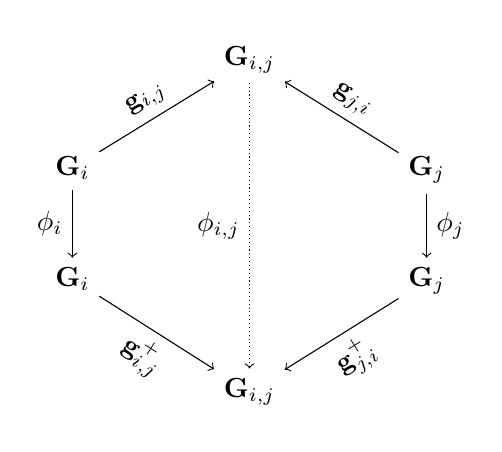
\begin{tikzpicture}
  \matrix[matrix of math nodes,column sep={64pt,between origins},row
%    sep={40pt,between origins},nodes={asymmetrical rectangle}] (s)
    sep={40pt,between origins},nodes={rectangle}] (s)
  {
      &|[name=Gij]|\amgrpG_{i,j} &      \\
 |[name=Gi]|  \amgrpG_i     &  &|[name=Gj]| \amgrpG_j  \\
 |[name=Gpi]|  \amgrpG_i      &  &|[name=Gpj]| \amgrpG_j   \\
     &|[name=Gpij]|\amgrpG_{i,j} &    \\ };
  \draw[ ->]
 % \draw[right hook ->]
   (Gi) edge  node[sloped,above] {$\amg_{i,j}$} (Gij)
                    (Gpj) edge   node[sloped,below] {$\amg^+_{j,i}$}  (Gpij);
%  \draw[left hook ->] 
  \draw[ ->] 
                    (Gj) edge node[sloped,above] {$\amg_{j,i}$} (Gij)
         (Gpi) edge node[sloped,below] {$\amg^+_{i,j}$} (Gpij);
  \draw[->] 
(Gi) edge node[left] {$\phi_i$}  (Gpi)
(Gij) edge [densely dotted] node[left] {$\phi_{i,j}$}  (Gpij)
(Gj) edge node[right] {$\phi_j$}  (Gpj);  
\end{tikzpicture}
\end{center}
\caption{The commuting hexagon of Corollary~\ref{cor:completing the hexagon}.}\label{fig:completing the hexagon}
\end{figure}
\bco\label{cor:completing the hexagon}

With the notation introduced above, fix the maps $\gamma_{i,j},\gamma^+_{i,j}, \phi_i \in \amgrpC_i$ as well as 
 $\gamma_{j,i}\in \amgrpC_j$. 
Then for any one of $\gamma^+_{j,i}, \phi_j\in \amgrpC_j$, there exists a choice $\gamma\in \amgrpC_i$ for the remaining map in $\amgrpC_j$  so that there exists $\phi_{i,j}$ making the diagram in Figure~\ref{fig:completing the hexagon} commute.
Moreover, if $\liediag_{i,j}$ is one of $A_2$, $B_2$, $C_2$, $\twA_3$, then $\gamma$ is unique, whereas if $\liediag_{i,j}=\twD_3$, then there are exactly two choices for $\gamma$. 
\eco
\bpf
The first claim follows immediately from the fact that the restriction maps $\ama_{j,i}\colon \amgrpC_{i,j}\to \amgrpC_i$ and $\ama_{i,j}\colon \amgrpC_{i,j}\to \amgrpC_j$ in part 4.~and 5.~of Lemma~\ref{lem: coefficient system connecting maps}  are both surjective. The second claim follows from the fact that $\ama_{j,i}\colon \amgrpC_{i,j}\to\amgrpC_i$ is injective except if $\Gamma_{i,j}=\twD_3$ in which case it has a kernel of order $2$.
\epf

\medskip

\bpf (of Proposition~\ref{prop:trivial support on spanning tree})
By Lemma~\ref{lem:stripping tori from connecting maps} we may assume that $\amg_{i,j}=\famg_{i,j}\after\gamma_{i,j}$ for some $\gamma_{i,j}\in \amgrpC_i$ for all $i,j\in I$.

For any (possibly empty) subset $T\sbe\vrtc$ let $S(T)$ be the set of pairs $(i,j)\in S$ such that $i\in T$.
Clearly the trivial support of $\amG$ contains $S(\emptyset)$.

We now show that if $T$ is the vertex set of a (possibly empty) proper subtree of $\Sigma$, and $u$ is a vertex such that $T\cup \{u\}$ is also the vertex set of a subtree of $\Sigma$, then for any  Curtis-Tits amalgam $\amG$ whose trivial support contains $S(T)$, there is a  Curtis-Tits amalgam $\amG^+$ isomorphic to $\amG$, whose trivial support contains $S(T\cup\{u\})$.

Once this is proved, Claim 1.~follows since we can start with $T=\emptyset$ and end with a  Curtis-Tits amalgam, still isomorphic to $\amG$, whose trivial support contains $S$.

Now let $T$ and $u$ be as above. 
We first deal with the case where $T\ne\emptyset$. 
Let $t$ be the unique neighbor of $u$ in the subtree of $\Sigma$ with vertex set $T\cup\{u\}$.
We shall define an amalgam $\amG^+=\{\amgrpG_i,\amgrpG_{i,j},\amg_{i,j}^+=\famg_{i,j}\after\gamma^+_{i,j}\mid i,j\in I\}$ and an isomorphism
 $\phi\colon \amG\to \amG^+$, where $\gamma^+_{i,j},\phi_i\in \amgrpC_i$ and $\phi_{\{i,j\}}\in \amgrpC_{i,j}$ for all $i,j\in I$. 
First note that it suffices to define $\amg^+_{i,j}$, $\phi_i$ and $\phi_{\{i,j\}}$ for $\{i,j\}\in \edg$: given this data, by the $A_1\times A_1$ case in Lemma~\ref{lem:coefficient system groups} and Lemma~\ref{cor:completing the hexagon}, for any non-edge $\{k,l\}$ there is a unique $\phi_{\{k,l\}}\in \amgrpC_{k,l}$ such that 
 $(\phi_{k,l},\phi_k,\phi_l)$ is an isomorphism between  $\amG_{\{k,l\}}$ and $\amG^+_{\{k,l\}}$.

Before defining inclusion maps on edges, note that since $\liediag$ is $3$-spherical, no two neighbors of $u$ in $\Gamma$ are connected by an edge.
Therefore we can unambiguously set 
\begin{align*}
\amg^+_{i,j} & = \amg_{i,j}  \mbox{ for }u\not\in\{i,j\}\in \edg\liediag. 
\end{align*} 
Note that both maps $\amg^+_{t,u}$ and $\amg^+_{u,t}$ are forced upon us, but at  this point for any other neighbor $v$ of $u$, only one of $\amg^+_{u,v}$ and $\amg^+_{v,u}$ is forced upon us. 
We set 
\begin{align*}
\amg^+_{t,u}&=\amg_{t,u}, \mbox{ and }\\
\amg^+_{v,u}&=\amg_{v,u} \mbox{ for }v\in I \mbox{ with }(u,v)\not\in S \mbox{ and }(v,u)\in S.
\end{align*}
To extend the trivial support as required, we set 
\begin{align*}
\amg^+_{u,v}&=\famg_{u,v} \mbox{ for }v\in I \mbox{ with }(u,v)\in S.
\end{align*}
We can already specify part of $\phi$: Set
\begin{align*}
\phi_i& =\id_{\amgrpG_i} \mbox{ for }i\in I-\{u\},\\
\phi_{\{i,j\}}&=\id_{\amgrpG_{i,j}} \mbox{ for } u\not\in \{i,j\}\in \edg\liediag.
\end{align*}
Thus, what is left to specify is the following: $\phi_u$ and $\phi_{\{u,t\}}$ and, for all neighbors $v\ne t$ of $u$ we must specify $\phi_{\{u,v\}}$ as well as  
\begin{align*}
\amg^+_{u,v} & \mbox{ if  } (u,v)\not\in S,\\
\amg^+_{v,u} & \mbox{ if }  (u,v)\in S.
\end{align*}  

Figures~\ref{fig:vu not in S}~and~\ref{fig:uv not in S} describe the amalgam $\amG$ (top half) and $\amG^+$ (bottom half) at the vertex $u$, where $t\in \vrtc \Sigma$, $v\in \vrtc \liediag$, and $\{u,t\}, \{u,v\}\in \edg\liediag$.
Inclusion maps from $\amG^+$ forced upon us are indicated in bold, the dotted arrows are those we must define so as to make the diagram commute.

\begin{figure}[H]
\begin{center}
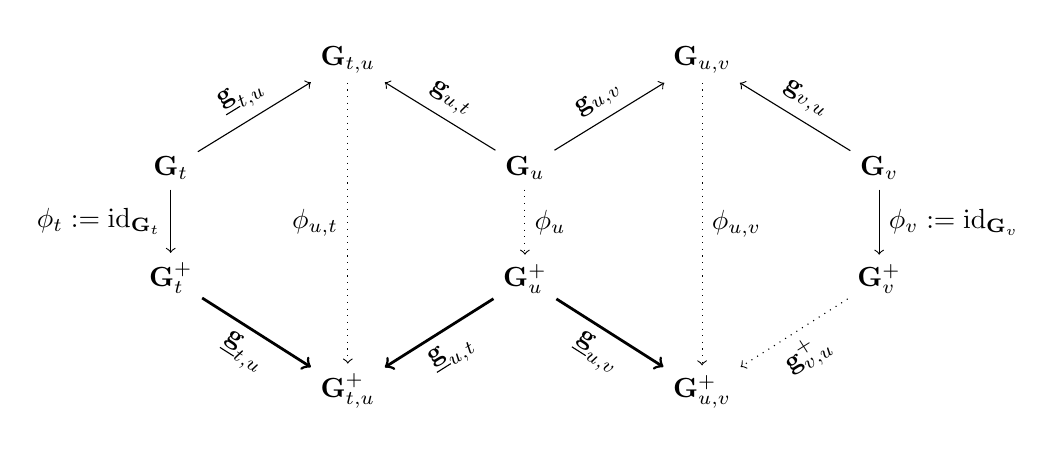
\begin{tikzpicture}
  \matrix[matrix of math nodes,column sep={64pt,between origins},row
%    sep={40pt,between origins},nodes={asymmetrical rectangle}] (s)
    sep={40pt,between origins},nodes={rectangle}] (s)
  {
      &|[name=Gtu]|\amgrpG_{t,u} & &|[name=Guv]| \amgrpG_{u,v} &     \\
 |[name=Gt]|  \amgrpG_t      &  &|[name=Gu]| \amgrpG_u& & |[name=Gv]| \amgrpG_v    \\
 |[name=Gpt]|  \amgrpG^+_t      &  &|[name=Gpu]| \amgrpG^+_u&  & |[name=Gpv]| \amgrpG^+_v    \\
     &|[name=Gptu]|\amgrpG^+_{t,u} & &|[name=Gpuv]| \amgrpG^+_{u,v} &     \\
  };
%  \draw[right hook ->]
  \draw[ ->]
   (Gt) edge  node[sloped,above] {$\famg_{t,u}$} (Gtu)
              (Gu) edge  node[sloped,above] {$\amg_{u,v}$} (Guv)
                    (Gpu) edge [line width = 1pt]  node[sloped,below] {$\famg_{u,t}$}  (Gptu)
   (Gpv) edge [dotted] node[sloped,below] {$\amg^+_{v,u}$} (Gpuv)
 ;
 
 %\draw[left hook ->] 
 \draw[->] 
                    (Gu) edge   node[sloped,above] {$\amg_{u,t}$} (Gtu)
     (Gv) edge  node[sloped,above] {$\amg_{v,u}$} (Guv)
         (Gpu) edge  [line width = 1pt]  node[sloped,below] {$\famg_{u,v}$}  (Gpuv)
         (Gpt) edge  [line width = 1pt]  node[sloped,below] {$\famg_{t,u}$} (Gptu)
    ;
  
 \draw[->] 
(Gt) edge  node[left] {$\phi_t:=\id_{\amgrpG_t}$}  (Gpt)
(Gtu) edge [ dotted]  node[left] {$\phi_{u,t}$}  (Gptu)
(Gu) edge [ dotted]  node[right] {$\phi_u$}  (Gpu)
(Guv) edge [ dotted]  node[right] {$\phi_{u,v}$}  (Gpuv)
(Gv) edge  node[right] {$\phi_v:=\id_{\amgrpG_v}$}  (Gpv)
;  
\end{tikzpicture}
\caption{The case $(u,v)\in S$ and $(v,u)\not\in S$.}\label{fig:vu not in S}
\end{center}
\end{figure}
\begin{figure}[H]
\begin{center}
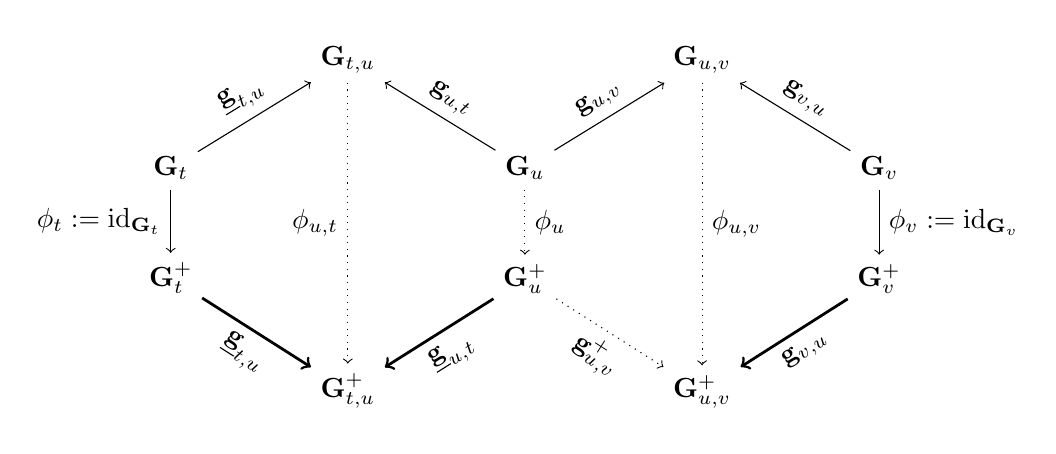
\begin{tikzpicture}
  \matrix[matrix of math nodes,column sep={64pt,between origins},row
%    sep={40pt,between origins},nodes={asymmetrical rectangle}] (s)
    sep={40pt,between origins},nodes={rectangle}] (s)
  {
      &|[name=Gtu]|\amgrpG_{t,u} & &|[name=Guv]| \amgrpG_{u,v} &     \\
 |[name=Gt]|  \amgrpG_t      &  &|[name=Gu]| \amgrpG_u& & |[name=Gv]| \amgrpG_v    \\
 |[name=Gpt]|  \amgrpG^+_t      &  &|[name=Gpu]| \amgrpG^+_u&  & |[name=Gpv]| \amgrpG^+_v    \\
     &|[name=Gptu]|\amgrpG^+_{t,u} & &|[name=Gpuv]| \amgrpG^+_{u,v} &     \\
  };
%  \draw[right hook ->]
  \draw[ ->]
   (Gt) edge  node[sloped,above] {$\famg_{t,u}$} (Gtu)
              (Gu) edge  node[sloped,above] {$\amg_{u,v}$} (Guv)
                    (Gpu) edge [line width = 1pt]  node[sloped,below] {$\famg_{u,t}$}  (Gptu)
   (Gpv) edge [line width = 1pt] node[sloped,below] {$\amg_{v,u}$} (Gpuv)
 ;
 
% \draw[left hook ->] 
 \draw[ ->] 
                    (Gu) edge   node[sloped,above] {$\amg_{u,t}$} (Gtu)
     (Gv) edge  node[sloped,above] {$\amg_{v,u}$} (Guv)
         (Gpu) edge [dotted] node[sloped,below] {$\amg^+_{u,v}$}  (Gpuv)
         (Gpt) edge  [line width = 1pt]  node[sloped,below] {$\famg_{t,u}$} (Gptu)
    ;
  
 \draw[->] 
(Gt) edge  node[left] {$\phi_t:=\id_{\amgrpG_t}$}  (Gpt)
(Gtu) edge [ dotted]  node[left] {$\phi_{u,t}$}  (Gptu)
(Gu) edge [ dotted]  node[right] {$\phi_u$}  (Gpu)
(Guv) edge [ dotted]  node[right] {$\phi_{u,v}$}  (Gpuv)
(Gv) edge  node[right] {$\phi_v:=\id_{\amgrpG_v}$}  (Gpv)
;  
\end{tikzpicture}
\caption{The case $(u,v)\not\in S$ and $(v,u)\in S$.}\label{fig:uv not in S}
\end{center}
\end{figure}
In these figures all non-dotted maps are of the form $\famg_{i,j}\after\gamma_{i,j}$ for some $\gamma_{i,j}\in \amgrpC_i$ hence we can find the desired maps using Corollary~\ref{cor:completing the hexagon}.


In case $T=\emptyset$, the situation is as described in Figures~\ref{fig:vu not in S}~and~\ref{fig:uv not in S} after removing the $\{u,t\}$-hexagon and any conditions it may impose on $\phi_u$, and letting $v$ run over all neighbors of $u$. That is, we must now define $\phi_u$, and for any neighbor $v$ of $u$, we must find $\phi_{u,v}$ as well as 
\begin{align*}
\amg^+_{u,v} & \mbox{ if  } (u,v)\not\in S,\\
\amg^+_{v,u} & \mbox{ if }  (u,v)\in S.
\end{align*}
To do so we let $\phi_u=\id_{\amgrpG_u}\in \amgrpC_u$. 
Finally, for each neighbor $v$ of $u$ we simply let $\amg_{u,v}^+=\amg_{u,v}$ (so that $\phi_{u,v}=\id_{\amgrpG_{i,j}}\in \amgrpC_{i,j}$) if $(u,v)\not\in S$, and we obtain $\amg^+_{v,u}$ and $\phi_{u,v}\in \amgrpC_{u,v}$ using Corollary~\ref{cor:completing the hexagon} if $(u,v)\in S$.
\epf

\subsection{Classification of  Curtis-Tits amalgams with $3$-spherical diagram}\label{subsec:classification of 3-spherical CT amalgams}

In the case where $\amG$ is a Curtis-Tits amalgam over $\FF_q$ whose diagram is a $3$-spherical tree,  Proposition~\ref{prop:trivial support on spanning tree} says that $\amG\cong\famG$. 

\bth\label{thm:CT 3 spherical tree}
Suppose that $\amG$ is a  Curtis-Tits amalgam with a diagram that is a $3$-spherical tree.
Then, $\amG$ is unique up to isomorphism. 
In particular any  Curtis-Tits amalgam with spherical diagram is unique.
\eth

\ble\label{lem:spanning tree with minimal complement}
Given a Curtis-Tits amalgam over $\FF_q$ with connected $3$-spherical diagram $\liediag$ there is a spanning tree $\Sigma$ such that the set of edges 
 in $\edg\liediag-\edg\Sigma=\{\{i_s,j_s\}\colon s=1,2,\ldots,r\}$ has the property that
 \begin{enumerate}
 \item\label{cond:A2} $(\amgrpG_{\{i_s,j_s\}},\amg_{i_s,j_s}(\amgrpG_{i_s}),\amg_{i_s,j_s}(\amgrpG_{j_s}))$ has type $A_2(q^{e_s})$, where $e_s$ is some power of $2$.
  \item\label{cond:minimal e} There is a loop $\Lambda_s$ containing $\{i_s,j_s\}$ such that 
  any vertex group of $\Lambda_s$ is isomorphic to $\SL_2(q^{e_s 2^l})$ for some $l\ge 0$.  
 \end{enumerate}
\ele
\bpf
Induction on the rank $r$ of  $H^1(\liediag,\ZZ)$.
If $r=0$, then there is no loop at all and we are done.

Consider the collection of all edges $\{i,j\}$ of $\Gamma$ such that $\liediag_{\{i,j\}}$ has type $A_2$ and 
 $H^1(\liediag-\{i,j\},\ZZ)$ has rank $r-1$, and choose one such that $\amgrpG_i\cong\SL_2(q^{e_1})$ where $e_1$ is minimal among all these edges.  
Next replace $\liediag$ by $\liediag-\{i,j\}$ and use induction.
Suppose $\{i_s,j_s\}\mid s=1,2,\ldots,r\}$ is the resulting selection of edges so that $\Sigma=\liediag-\{i_s,j_s\}\mid s=1,2,\ldots,r\}$ is a spanning tree and condition~\eqref{cond:A2} is satisfied.
Note that by choice of these edges, also condition~\eqref{cond:minimal e} is satisfied by at least one of the loops of $\liediag-\{\{i_t,j_t\}\colon t=1,2,\ldots,s-1\}$ that contains $\{i_s,j_s\}$.
Note that this uses the fact that by $3$-sphericity every vertex belongs to at least one subdiagram of type $A_2$.
\epf



\bde\label{dfn:CT the map kappa}
Fix a connected $3$-spherical diagram $\liediag$ and a prime power $q$. Let  $\Sigma$  be a spanning tree and let the set of edges $\edg\liediag-\edg\Sigma=\{\{i_s,j_s\}\colon s=1,2,\ldots,r\}$ together with the integers $\{e_s\colon s=1,2,\ldots,r\}$ satisfy the conclusions of Lemma~\ref{lem:spanning tree with minimal complement}.
Let $\sCT(\liediag,q)$ be the collection of isomorphism classes of  Curtis-Tits amalgams of type $\liediag(q)$ and let $\famG=\{\amgrpG_i,\amgrpG_{i,j},\famg_{i,j}\mid i,j\in I\}$ be the standard Curtis-Tits amalgam over $\FF_q$ with diagram $\liediag$ as in Subsection~\ref{subsec:trivial support}.

Consider the following map:
\begin{align*}
\kappa\colon\prod_{s=1}^r \Aut(\FF_{q^{e_s}})\times \langle\trin\rangle\to \sCT(\liediag).
\end{align*}
where $\kappa((\alpha_s)_{s=1}^r)$ is the isomorphism class of the amalgam $\amG^+=\amG((\alpha_s)_{s=1}^r)$ given by setting $\amg^+_{j_s,i_s}=\famg_{j_s,i_s}\after \alpha_s$ for all $s=1,2,\ldots,r$.
\ede

We now have 
\bco\label{cor:CT kappa is onto}
The map $\kappa$ is onto.
\eco
\bpf
Note that, for each $s=1,2,\ldots,r$, the Curtis-Tits standard pair $(\amgrpG_{\{i_s,j_s\}}$, $\amg_{i_s,j_s}(\amgrpG_{i_s})$, $\amg_{i_s,j_s}(\amgrpG_{j_s}))$ has type $A_2(q^{e_s})$ and so $\amgrpC_{j_s}=\Aut(\FF_{q^{e_s}})$.  Thus the claim is an immediate consequence of Proposition~\ref{prop:trivial support on spanning tree}.
\epf

\medskip
We note that if we select $\Sigma$ differently, the map $\kappa$ will still be onto. However, the ``minimal'' choice made in Lemma~\ref{lem:spanning tree with minimal complement} ensures that $\kappa$ is injective as well, as we will see.

\ble\label{lem:classification of  CT amalgams with loop diagram}
Suppose $\liediag(q)$ is a 
$3$-spherical diagram $\liediag$ that is a simple loop. 
Then, $\kappa$ is injective.
\ele
\bpf
Suppose there is an isomorphism $\kappa(\alpha)=\amG\stackrel{\phi}{\longrightarrow} \amG^+=\kappa(\beta)$, for some  $\alpha,\beta\in \Aut(\FF_q)\times\langle \trin\rangle$.
 Write $I=\{0,1,\ldots,n-1\}$ so that $\{i,i+1\}\in \edg\liediag$ for all $i\in I$ (subscripts modulo $n$).
 Without loss of generality assume that $(i_1,j_1)=(1,0)$ so that by Proposition~\ref{prop:trivial support on spanning tree} we  may assume that $\amg_{i,j}=\famg_{i,j}=\amg^+_{i,j}$ for all $(i,j)\ne (1,0)$.
This means that  $\ama\colon \amgrpC_{i,i+1}\to \amgrpC_i\times\amgrpC_{i+1}$ sends $\phi_{i,i+1}$ to $(\phi_i,\phi_{i+1})$ for any edge $\{i,i+1\}\ne \{0,1\}$. 
Now note that by minimality of $q$, $\amgrpC_i$  (and $\amgrpC_{i,i+1}$) has a quotient $\bar{\amgrpC}_i$   (and $\bar{\amgrpC}_{i,i+1}$) isomorphic to $\langle\Aut(\FF_q)\rangle\times\langle\trin\rangle$ for every $i\in I$, by considering the action of $\amgrpC_i$ on the subgroup of $\amgrpG_i$ isomorphic to $\SL_2(q)$. 
By Part 4 and 5 of Lemma~\ref{lem: coefficient system connecting maps} the maps  $\ama_{i+1,i}^{-1}$ and $\ama_{i,i+1}$ induce isomorphisms $\bar{\amgrpC}_i\to \bar{\amgrpC}_{i,i+1}$ and $\bar{\amgrpC}_{i,i+1}\to\bar{\amgrpC}_{i+1}$, which compose to an isomorphism
\begin{align*}
\phi_i&\mapsto \famg_{i+1,i}^{-1}\after \famg_{i,i+1}\after \phi_i \after \famg_{i,i+1}^{-1}\after \famg_{i+1,i},
\end{align*}
sending the image of $\trin$ and $\alpha$ in $\bar{\amgrpC}_i$ to the image of $\trin$ (and $\alpha$ respectively) in $\bar{\amgrpC}_{i+1}$, where $\alpha\colon x\mapsto x^p$ for $x$ in the appropriate extension of $\FF_q$ defining $\amgrpG_{i,i+1}$. 
Concatenating these maps along the path $\{1,2,\ldots,n-1,0\}$ and considering the edge $\{0,1\}$ we see that the images of $\beta^{-1}\phi_1\alpha$ and $\phi_1$ in $\bar{\amgrpC}_1=\amgrpC_1$ coincide.
 Since $\amgrpC_1$ is abelian this means that $\beta=\alpha$.
\epf








\bth\label{thm:CT classification of 3-spherical amalgams}
Let  $\liediag$ be a connected $3$-spherical diagram with spanning tree $\Sigma$ and set of edges
 $\edg\liediag-\edg\Sigma=\{\{i_s,j_s\}\colon s=1,2,\ldots,r\}$ together with the integers $\{e_s\colon s=1,2,\ldots,r\}$ satisfying the conclusions of Lemma~\ref{lem:spanning tree with minimal complement}.
Then $\kappa$ is a bijection between the elements of $\prod_{s=1}^r \Aut(\FF_{q^{e_s}})\times \langle\trin\rangle$ and the type preserving isomorphism classes of  Curtis-Tits amalgams with diagram $\liediag$ over $\FF_q$.
\eth
\bpf
Again, it suffices to show that $\kappa$ is injective. This in turn follows from Lemma~\ref{lem:classification of  CT amalgams with loop diagram}, for if two amalgams are isomorphic (via a type preserving isomorphism), then the amalgams induced on subgraphs of $\liediag$ must be isomorphic and Lemma~\ref{lem:classification of  CT amalgams with loop diagram} shows that $\kappa$ is injective on the subamalgams supported by the loops $\Lambda_s$ ($s=1,2,\ldots,r$).
\epf
\section{Classification of  Phan amalgams}\label{sec:classification of Ph amalgams}
\subsection{Introduction}
The classification problem is formulated as follows: Determine, up to isomorphism of amalgams, all  Phan amalgams $\amG$ with given diagram $\liediag$ possessing a non-trivial (universal) completion.

\subsection{Classification of Phan amalgams with $3$-spherical diagram}
\subsubsection{Tori in Phan standard pairs}\label{subsubsec:Tori Phan standard pairs}
Let $\amG=\{\amgrpG_{i,j},\amgrpG_i,\amg_{i,j}\mid i,j\in I\}$ be a Phan amalgam over $\FF_q$ with $3$-spherical diagram $\liediag=(I,E)$.
This means that the subdiagram of $\liediag$ induced on any set of three vertices is spherical.
This is equivalent to $\liediag$ not containing triangles of any kind and such that no vertex is on more than one $C_2$-edge.

\bde\label{dfn:tori in phan amalgam}
For any $i,j\in I$ with $\{i,j\}\in \edg\liediag$, let 
\begin{align*}
\amgrpD_i^j=N_{\amgrpG_{i,j}}(\amg_{j,i}(\amgrpG_j))\cap \amg_{i,j}(\amgrpG_i)
\end{align*}
\ede
\ble\label{lem:tori in phan standard pairs}
Suppose that $(\amgrpG,\amgrpG_1,\amgrpG_2)$ is a Phan standard pair of type 
$\liediag(q)$ as in Subsection~\ref{subsec:standard P pairs}. 
\begin{enumerate}
\item If $\liediag(q)=A_2(q)$, then $\langle \amgrpD_1^2, \amgrpD_2^1\rangle$ is the standard torus stabilizing the orthonormal basis $\{e_1,e_2,e_3\}$. Here $\amgrpD_1^2$ (resp. $\amgrpD_2^1$) is the stabilizer in this torus of $e_1$ (resp. $e_3$).
\item If $\liediag(q)=C_2(q)$, then $\langle \amgrpD_1^2,\amgrpD_2^1\rangle$ is the standard torus stabilizing the 
 basis $\{e_1,e_2,e_3=f_1,e_4=f_2\}$ which is hyperbolic for the symplectic form of $\Sp_4(q^2)$ and orthonormal for the unitary form of $\SU_4(q)$; Here $\amgrpD_2^1$ (resp. $\amgrpD_1^2$) is the stabilizer of $\langle e_2\rangle$ and $\langle f_2\rangle$ (resp.~the pointwise stabilizer of both $\langle e_1,f_1\rangle$ and $\langle e_2,f_2\rangle$).
Thus, 
\begin{align*}
\amgrpD_2^1&=\langle\diag(1,a,1,a^\sigma)\colon a\in \FF_{q^2}\mbox{ with }aa^\sigma=a^{q+1}=1\rangle,\\
\amgrpD_1^2&=\langle\diag(a,a^\sigma,a^\sigma,a )\colon a\in \FF_{q^2}\mbox{ with }aa^\sigma=a^{q+1}=1\rangle.
\end{align*}
\item In either case, for $\{i,j\}=\{1,2\}$,  $\amgrpD_i^j=C_{\amgrpG_{i,j}}(\amgrpD_j^i)\cap\amgrpG_i$ and 
 $\amgrpD_j^i$ is the unique torus of $\amgrpG_j$ normalized by $\amgrpD_i^j$. 
\end{enumerate}
\ele
\bpf
Parts 1.~and~2.~as well as the first claim of Part 3.~are straightforward matrix calculations.
As for the last claim note that in both cases, $\amgrpD_i^j$ acts diagonally on $\amgrpG_j$ viewed as $\SU_2(q)$ in it natural representation $V$ via the standard identification map; in fact  (in the case $C_2$, $\amgrpD_2^1$ acts even innerly on $\amgrpG_1$).
If $\amgrpD_i^j$ normalizes a torus $\amgrpD'$ in $\amgrpG_j$ then it will have to stabilize its eigenspaces.
Since $q+1\ge 3$, the eigenspaces of $\amgrpD_i^j$ in its action on $V$ have dimension $1$, so $\amgrpD_i^j$ and $\amgrpD'$ must share these eigenspaces. This means that $\amgrpD'=\amgrpD_j^i$.
\epf

\subsubsection{Property (D) for Phan amalgams}\label{subsubsec:Phan property D}
We state Property (D) for $3$-spherical Phan amalgams, extending the definition from~\cite{BloHof2014b} which was given for Curtis-Tits amalgams under the assumption that $q\ge 4$.
\bde\label{dfn:property D}\nom{{(\rm property (D))}}{}
We say that $\amG$ {\dfn has property (D)} if there is a {\dfn system of tori} $\cD=\{\amgrpD_i\colon i\in I\}$ such that for all edges $\{i,j\}\in \edg\liediag$ we have  $\amg_{i,j}(\amgrpD_i)=\amgrpD_i^j$.
\ede
\ble\label{lem:non-collapsing Phan has property D}
Suppose that $\amG$ has a completion $(\compG,\compg)$ so that $\compg_i$ is non-trivial for all $i\in I$.
Then, for any $i,j,k\in I$ such that $\{i,j\},\{j,k\}\in \edg\liediag$, there is a torus $\amgrpD_j\le \amgrpG_j$ such that 
 $\amg_{j,i}(\amgrpD_j)=\amgrpD_j^i$ and $\amg_{j,k}(\amgrpD_j)=\amgrpD_j^k$.
In particular, $\amG$ has property (D).
\ele
\bpf
First note that in case $q=2$, the conclusion of the lemma is trivially true as, for all $i\in I$, $\amgrpG_i\cong S_3$ has a unique Phan torus.

We now consider the general case.
For $\liediag(q)=A_3(q)$, this was proved by Bennett and Shpectorov in~\cite{BeSh2004} (see also~\cite{BloHof2014b}).
For completeness we recall the argument, which applies in this more general case as well.
We shall prove that 
 \begin{align*}
 \compg(\amgrpD_j^i)&=\compg(\amgrpD_j^k)
 \end{align*}
and then let  $\amgrpD_j\le \amgrpG_j$ be such that $\compg(\amgrpD_j)= \compg(\amgrpD_j^i)=\compg(\amgrpD_j^k)$.
Note that since $\compg_j$ is non-trivial, it now follows that $\amg_{j,i}(\amgrpD_j)=\amgrpD_j^i$ and $\amg_{j,k}(\amgrpD_j)=\amgrpD_j^k$.

Recall that for any subgroup $\amgrpH$ of a group in $\amG$ we'll write $H=\compg(\amgrpH)$.
We show that $D_j^i$ is normalized by $D_k^j$ and use Lemma~\ref{lem:tori in phan standard pairs} to conclude that 
 $D_j^i=D_j^k$.
To that end we let $h\in D_k^j$  and prove that $hD_j^ih^{-1}=D_j^i$. To achieve this we show that $hD_j^ih^{-1}$ is normalized by $D_i^j$ and again use Lemma~\ref{lem:tori in phan standard pairs}.
So now let $g\in D_i^j$ and 
note that since $\liediag$ is $3$-spherical, $\{i,k\}\not\in \edg\liediag$ so that $g$ and $h$ commute.
In addition note that  by Lemma~\ref{lem:tori in phan standard pairs},  $gD_j^ig^{-1}=D_j^i$.
Therefore we have 
\begin{align*}
ghD_j^i h^{-1}g^{-1}= hg D_j^i g^{-1}h^{-1}= h D_j^i h^{-1},
\end{align*}
as required.
\epf

\subsubsection{The coefficient system of a  Phan amalgam}\label{subsec:Phan coefficient system}

\bde\label{dfn:type of P amalgam}
We now fix a standard Phan amalgam  $\famG=\{\amgrpG_i,\amgrpG_{i,j},\famg_{i,j}\mid i,j\in I\}$ over $\FF_q$ with diagram $\liediag(q)$, where for every $i,j\in I$, $\famg_{i,j}$ is the standard identification map of Definition~\ref{dfn:standard Phan identification map}.
Then,  $\famG$ has property (D) with system of tori $\cD=\{\amgrpD_i\colon i\in I\}$ as in Lemma~\ref{lem:tori in phan standard pairs}. 

If $\amG$ is any other  non-collapsing Phan amalgam over $\FF_q$ with diagram $\liediag$, then since all tori of $\amgrpG_i$ are conjugate under $\Aut(\amgrpG_i)$, by adjusting the inclusion maps $\amg_{i,j}$ we can replace $\amG$ by an isomorphic amalgam whose system of tori is exactly $\cD$.
\ede


From now on we assume that $\famG$, $\cD=\{\amgrpD_i\colon i\in I\}$ and $\amG$ are as in Definition~\ref{dfn:type of P amalgam}


\bde\label{dfn:phan coefficient system}
Suppose that $\amG=\{\amgrpG_i,\amgrpG_{i,j},\amg_{i,j}\mid i,j\in I\}$ is a Phan amalgam with connected $3$-spherical diagram $\liediag$ having property (D).
Let $\cD=\{\amgrpD_i\colon i\in I\}$  be the associated system of  tori.
The {\dfn coefficient system associated to $\amG$} is the collection 
 $\amA=\{\amgrpA_i,\amgrpA_{i,j},\ama_{i,j}\mid i,j\in I\}$ where, for any $i,j\in I$ we set 
 \begin{align*}
 \amgrpA_i&=N_{\Aut(\amgrpG_i)}(\amgrpD_i), \\
 \amgrpA_{i,j}&=N_{\Aut(\amgrpG_{i,j})}(\amg_{i,j}(\amgrpG_i))\cap N_{\Aut(\amgrpG_{i,j})}(\amg_{j,i}(\amgrpG_j)), \\
 \ama_{i,j}&\colon \amgrpA_{i,j}\to\amgrpA_j \mbox{ is given by restriction: } \varphi\mapsto \amg_{j,i}^{-1}\after \rho_{i,j}(\varphi)\after\amg_{j,i}.
  \end{align*}
where $\rho_{i,j}(\varphi)$ is the restriction of $\varphi$ to $\bamgrpG_j\le \amgrpG_{i,j}$.
\ede
From now on we let $\amA$ be the coefficient system associated to $\famG$ with respect to the system of tori $\cD$.
The fact that the $\ama_{i,j}$ are well-defined follows from the following simple observation.
\ble\label{lem:N G1 G2=N D1 D2} 
For any $i,j\in I$ with $\{i,j\}\in \edg\liediag$, we have 
\begin{align*}
\amgrpA_{i,j}\le N_{\Aut(\amgrpG_{i,j})}(\amg_{i,j}(\amgrpD_i))\cap N_{\Aut(\amgrpG_{i,j})}(\amg_{j,i}(\amgrpD_j)).
\end{align*}
\ele
\bpf
The inclusion $\le$ is immediate from the definitions.
\epf

\medskip

The significance for the classification of  Phan  amalgams with the same system of tori is as follows:
\bpr\label{prop:P coefficient systems}
Suppose that $\amG$ and $\amG^+$ are  Phan amalgams of type $\famG$ with the same system of tori $\cD=\{\amgrpD_i\colon i\in I\}$.
\begin{enumerate}
\item For all $i,j\in I$, we have $\amg_{i,j}=\famg_{i,j}\after\delta_{i,j}$ and $\amg_{i,j}=\famg_{i,j}\after\delta_{i,j}^+$ for some $\delta_{i,j}, \delta_{i,j}^+\in \amgrpA_i$,
\item For any isomorphism $\phi\colon \amG\to\amG^+$ and $i,j\in I$, we have $\phi_i\in \amgrpA_i$, $\phi_{\{i,j\}}\in \amgrpA_{i,j}$, and $\ama_{i,j}(\phi_{\{i,j\}})=\delta_{i,j}^+\after\phi_i\after\delta_{i,j}^{-1}$.
\end{enumerate}
\epr
\bpf
Part 1.~follows since, for any $i,j\in I$ we have $\amg_{i,j}^{-1}\after\famg_{i,j}\in \Aut(\amgrpG_i)$ and  
\begin{align*}
\amg_{i,j}(\amgrpD_i)=\famg_{i,j}(\amgrpD_i).
\end{align*}
Part 2.~follows from Lemma~\ref{lem:N G1 G2=N D1 D2} since, for any $i,j\in I$,  
\begin{align*}
(\amgrpG_{i,j},\amg_{i,j}(\amgrpG_i),\amg_{j,i}(\amgrpG_j))
=(\amgrpG_{i,j},\famg_{i,j}(\amgrpG_i),\famg_{j,i}(\amgrpG_j)) =(\amgrpG_{i,j},\amg^+_{i,j}(\amgrpG_i),\amg^+_{j,i}(\amgrpG_j)).
\end{align*}
\epf

We now determine the groups appearing in a coefficient system by looking at standard pairs.
\ble\label{lem:structure of Phan A_i groups}
Fix $i\in I$ and let $q$ be such that $\amgrpG_i\cong\SU_2(q)$.
Then, 
\begin{align*}
\amgrpA_i&=\amgrpT_i\rtimes \amgrpC_i,
\end{align*}
where $\amgrpT_i$ is the subgroup of diagonal automorphisms in $\PGU_2(q)$ and $\amgrpC_i=\Aut(\FF_{q^2})$.
%\langle \trin, \Aut(\FF_q)\rangle$.
\ele
\bpf
This follows from the fact that via the standard embedding map $\famg_{i,j}$ the groups $\amgrpD_i$  of the system of tori are the subgroups of standard diagonal matrices in $\SU_2(q)$.

To see this note that $\amgrpG_i\cong\SU_2(q)$ and that $\Aut(\amgrpG_i)\cong\PGU_2(q)\rtimes\Aut(\FF_{q^2})$.
Also, $\amgrpD_i=\langle d\rangle$ for some $d=\diag(\zeta,\zeta^q)$ and $\zeta$ a primitive $q+1$-th root of $1$ in $\FF_{q^2}$.
A quick calculation now shows that $\tau$ and  $\sigma$ are the same in their action, which is inner and one verifies that $N_{\GU_2(q)}(\amgrpD_i)=\langle \trin,\diag(a,b)\colon a,b\in \FF_q^2\rangle$.
\epf


\ble\label{lem:structure of Phan A_ij groups}
Let $\amA$ be the coefficient system associated to the standard Phan amalgam $\famG$ of type $\liediag(q)$ and the system of tori $\cD$.

If $\Gamma=A_1\times A_1$, we have $\amgrpG_{i,j}=\amgrpG_i\times\amgrpG_j$, $\famg_{i,j}$ and $\famg_{j,i}$ are identity maps, and  
\begin{align}
\amgrpA_{i,j}&=\amgrpA_i\times\amgrpA_j\cong \amgrpT_{i,j}\rtimes\amgrpC_{i,j}.\label{eqn:Phan N Xi Xj A1timesA1}
\end{align}
where $\amgrpT_{i,j}=\amgrpT_i\times\amgrpT_j$ and $\amgrpC_{i,j}=\amgrpC_i\times\amgrpC_j$.
Otherwise, 
\begin{align*}
\amgrpA_{i,j}&=\amgrpT_{i,j}\rtimes\amgrpC_{i,j},
\end{align*}
where 
 $\amgrpC_{i,j}=\Aut(\FF_{q^2})$ and  $\amgrpT_{i,j}$ denotes the image of the standard torus $\GD$ in $\Aut(\amgrpG_{i,j})$.
Note that $\GD$ is as follows 
\begin{alignat*}{2}
\langle \diag(a,b,c)\colon &    a,b,c\in \FF_{q^2}\mbox{ with } aa^\sigma=bb^\sigma=cc^\sigma=1 \rangle && \mbox{ if } \liediag=A_2,\\
\langle \diag(c^\sigma b, ab ,c,a^\sigma)\colon &   a,b,c\in \FF_{q^2}\mbox{ with } aa^\sigma=bb^\sigma=cc^\sigma=1 \rangle && \mbox{ if } \liediag=C_2.
\end{alignat*}
\ele

\bre
\begin{enumerate}
\item In case $\liediag=C_2$, $\amgrpG\cong\Sp_4(q)$ is realized as $\Sp_4(q^2)\cap \SU_4(q)$
 with respect to a basis that is 
 hyperbolic for the symplectic form and orthonormal for the unitary form, and $\Aut(\FF_{q^2})$ acts entry-wise on these matrices. 
Moreover, $\tau$ acts as transpose-inverse on these matrices.
\item In all cases $\trin$ coincides with $\sigma$. 
\end{enumerate}
\ere

\bpf
The $A_1\times A_1$ case is self evident.
Now consider the case $\liediag=A_2$.
As in the proof of Lemma~\ref{lem:structure of Phan A_i groups}, $\Aut(\FF_{q^2})\le N_{\Aut(\amgrpG_{i,j})}(\amgrpG_i)\cap N_{\Aut(\amgrpG_{i,j})}(\amgrpG_j)$, $A^\trin={}^tA^{-1}=A^\sigma$ and $\Aut(\amgrpG_{i,j})\cong\PGU_3(q)\rtimes\Aut(\FF_{q^2})$, so it suffices to consider linear automorphisms.
As before this is an uncomplicated calculation.

Now consider the case $\liediag=C_2$. Writing $\GamL(V)\cong \GL_4(q^2)\rtimes\Aut(\FF_{q^2})$ with respect to the basis $\cE=\{e_1,e_2,e_3=f_1,e_4=f_2\}$, which is hyperbolic for the symplectic form of $\Sp_4(q^2)$ and orthonormal for the unitary form of $\SU_4(q)$, we have $\amgrpG_{i,j}=\Sp_4(q^2)\cap \SU_4(q)$.

There is an isomorphism $\Phi\colon \amgrpG_{i,j}\to \Sp_4(q)$ as in~\cite{GraHofShp2003}.
Abstractly, we have  $\Aut(\Sp_4(q))= \GSp_4(q)\rtimes\Aut(\FF_q)$ (with respect to a suitable basis $\sfE$ for $V$).
Since the embedding of $\Sp_4(q)$ into $\Sp_4(q^2)$ is non-standard, we are reconstructing the automorphism group here.

We first note that changing bases just replaces $\Aut(\FF_{q^2})$ with a different complement to the linear automorphism group.
As for linear automorphisms we claim that 
\begin{align*}
\GSp_4(q^2)\cap \GU_4(q)=\GSp_4(q)
\end{align*}
 (viewing the latter as a matrix group w.r.t.~$\sfE$).
Clearly, up to a center, we have  $\amgrpG_{i,j}\le \GSp_4(q^2)\cap \GU_4(q)\le \GSp_4(q)$ and we note that 
 $\GSp_4(q)/\Sp_4(q)\cong (\FF_q^*)^2/ (\FF_q^*)$.
Thus for $q$ even, the claim follows.
For $q$ odd, let $\FF_{q^2}^*=\langle \zeta\rangle$ and define  $\beta=\diag(\zeta^{q-1},\zeta^{q-1},1,1)$.
Then $\beta\in \GSp_4(q^2)\cap \GU_4(q)$ acts  
 on $\amgrpG_{i,j}$ as $\diag(\zeta^q,\zeta^q,\zeta,\zeta)$, which scales the symplectic form of $\Sp_4(q^2)$ by $\zeta^{q+1}$.
By~\cite{GraHofShp2003} the form of $\Sp_4(q)$ is proportional and since $\zeta^{q+1}$ is a non-square in $\FF_q$,  $\beta$ is a linear outer automorphism of $\Sp_4(q)$.  Thus, $\GSp_4(q)=\langle \Sp_4(q),\beta\rangle$ and the claim follows.

We now determine $\amgrpA_{i,j}$.
First we note that $\beta$, as well as the group $\Aut(\FF_{q^2})$ with respect to the basis $\cE$, clearly normalize $\amgrpG_i$ and $\amgrpG_j$ hence by Lemma~\ref{lem:N G1 G2=N D1 D2}, $\Aut(\FF_{q^2})\le \amgrpA_{i,j}$. So it suffices to determine inner automorphisms of $\Sp_4(q)$ normalizing $\amgrpD_i^j$ and $\amgrpD_j^i$.



Any inner automorphism in $\Sp_4(q)$ is induced by an inner automorphism of $\Sp_4(q^2)$.
So now the claim reduces to a matrix calculation in the group $\Sp_4(q^2)$.
\epf

\medskip

Next we describe the restriction maps $\ama_{i,j}$ for Phan amalgams made up of a single standard pair with trivial inclusion maps.


\ble\label{lem: Phan coefficient system connecting maps}
Let $\amA$ be the coefficient system of the standard Phan  amalgam $\famG$ over $\FF_q$ with diagram $\liediag$ and system of tori $\cD$. 
Fix $i,j\in I$ and let $(\amgrpG_{i,j},\bamgrpG_i,\bamgrpG_j)$ be a Phan standard pair in $\famG$ with diagram $\liediag_{i,j}$. Denote $\ama=(\ama_{j,i},\ama_{i,j})\colon \amgrpA_{i,j}\to \amgrpA_i\times\amgrpA_j$.
Then, we have the following:
\begin{enumerate}
\item If $\liediag_{i,j}=A_1\times A_1$, then $\ama$ is an isomorphism inducing $\amgrpT_{i,j}\cong\amgrpT_i\times\amgrpT_j$ and $\amgrpC_{i,j}\cong\amgrpC_i\times\amgrpC_j$.
\item If $\liediag_{i,j}=A_2$ or $C_2$, then $\ama$ induces an isomorphism $\amgrpT_{i,j}\to \amgrpT_i\times\amgrpT_j$.
\item If $\liediag(q)=A_2(q)$ or $\liediag(q)=C_2(q)$, then $\ama\colon\amgrpC_{i,j}\to \amgrpC_i\times\amgrpC_j$ is given by 
  $\alpha\mapsto (\alpha,\alpha)$ (for $\alpha\in \Aut(\FF_{q^2})$) which is a diagonal  embedding.
\end{enumerate}
\ele
\bpf
1.~ This is immediate from Lemma~\ref{lem:structure of Phan A_ij groups}.

For the remaining cases, recall that for any $\varphi\in \amgrpA_{i,j}$, we have 
 $\ama_{i,j}\colon \varphi\mapsto \famg_{j,i}^{-1}\after \rho_{i,j}(\varphi)\after\famg_{j,i}$, 
where $\rho_{i,j}(\varphi)$ is the restriction of $\varphi$ to $\bamgrpG_j\le \amgrpG_{i,j}$ (Definition~\ref{dfn:phan coefficient system}) and $\famg_{i,j}$ is the standard identification map of Definition~\ref{dfn:standard Phan identification map}.
Note that the standard identification map transforms the automorphism $\rho_{j,i}(\varphi)$ of $\bamgrpG_i$ essentially to the ``same" automorphism $\varphi$ of $\amgrpG_i$.

First let $\liediag(q)=A_2(q)$.
The map $\ama$ is well-defined. On $\GD$, it is induced by the homomorphism
 \begin{align*}
\diag(ac,c,ec) \mapsto (\diag(1,e), \diag(a,1)), 
 \end{align*}
where $a,c,e\in \FF_{q^2}$ are such that $aa^\sigma=cc^\sigma=ee^\sigma=1$.
Note that the kernel is $Z(\GD)$ so that $\ama$ is injective. The map is obviously surjective, so we are done.
Thus if we factor $\ama$ by $\amgrpT_{i,j}$ and $\amgrpT_i\times\amgrpT_j$, we get
\begin{align}
\amgrpC_{i,j}  \into &  \amgrpC_i\times\amgrpC_j \label{eqn:rho mod PGD}
 \end{align}
which is a diagonal embedding given by $\alpha^r\mapsto (\alpha^r,\alpha^r)$, where 
  $r\in \NN$ and $\alpha\colon x\mapsto x^p$ for $x\in \FF_{q^2}$.

Next let $\liediag(q)=C_2(q)$.
We can rewrite the elements of $\GD$ as 
 a diagonal matrix $\diag(xyz, xz, z y^{-1}, z)$, by taking $z=a^{\sigma}$, $y=(ac)^{-1}$, $x=a^2b$.
On $\GD$ the map $\ama$ is induced by the homomorphism 
 \begin{align*}
\diag(xyz,xz,y^{-1}z,z) \mapsto (\diag(y,1),\diag(x,1))
 \end{align*}
with kernel $\{\diag(z,z,z,z)\colon z\in \FF_{q^2} \mbox{ with }zz^\sigma=1\}=Z(\GU_4(q))$. 
Clearly $\ama\colon\amgrpT_{i,j}\to \amgrpT_i\times\amgrpT_j$ is an isomorphism.
Taking the quotient over these groups, $\ama$ induces a diagonal embedding as in~\eqref{eqn:rho mod PGD}, where we now interpret it in the $C_2(q)$ setting.
\epf

\medskip
\subsubsection{A standard form for Phan amalgams}\label{subsec:Phan trivial support}

Suppose that $\famG=\{\amgrpG_i,\amgrpG_{i,j},\famg_{i,j}\mid i,j\in I\}$ is a Phan amalgam over $\FF_q$ with $3$-spherical diagram $\liediag$.
Without loss of generality we will assume that all inclusion maps $\famg_{i,j}$ are the standard identification maps of Definition~\ref{dfn:standard Phan identification map}.
By Lemma~\ref{lem:non-collapsing Phan has property D}, $\famG$ has Property (D) and possesses a system 
 $\cD=\{\amgrpD_i\colon i\in I\}$ of tori, which, as noted in Definition~\ref{dfn:type of P amalgam} via the standard embeddings $\famg_{i,j}$ can be identified with those given in Lemma~\ref{lem:tori in phan standard pairs}.

We wish to classify all  Phan amalgams  $\amG=\{\amgrpG_i,\amgrpG_{i,j},\amg_{i,j}\mid i,j\in I\}$ over $\FF_q$ with the same diagram as $\famG$.
As noted in Definition~\ref{dfn:type of P amalgam} we may assume that all such amalgams share $\cD$.
Let $\amA=\{\amgrpA_i,\amgrpA_{i,j},\ama_{i,j}\mid i,j\in I\}$ be the coefficient system of $\famG$ associated to $\cD$.
By Proposition~\ref{prop:P coefficient systems}, we may restrict to those amalgams whose connecting maps 
 are of the form $\amg_{i,j}=\famg_{i,j}\after \delta_{i,j}$ for $\delta_{i,j}\in \amgrpA_i$ for all $i\in I$.

\bde\label{dfn:Phan trivial support}
The {\dfn trivial support} of $\amG$ (with respect to $\famG$) is the set $\{(i,j)\in I\times I\mid \amg_{i,j}=\famg_{i,j}\}$ (that is, $\delta_{i,j}=\id_{\amgrpG_i}$ in the notation of Proposition~\ref{prop:P coefficient systems}).
The word ``trivial'' derives from the assumption that the $\famg_{i,j}$'s are the standard identification maps of Definition~\ref{dfn:standard Phan identification map}.
\ede

Fix some spanning tree $\Sigma\sbe \Gamma$ and suppose that $\edg-\edg\Sigma=\{\{i_s,j_s\}\colon s=1,2,\ldots,r\}$
 so that $H_1(\Gamma,\ZZ)\cong\ZZ^r$. 
We now have 
\bpr\label{prop:Phan trivial support on spanning tree}
There is a  Phan amalgam $\amG(\Sigma)$ with the same diagram as $\famG$ and the same $\cD$, which is isomorphic to $\amG$ and has the following properties:
\begin{enumerate}
\item $\amG$ has trivial support $S=\{(i,j)\in I\times I\mid \{i,j\}\in \edg \Sigma\}\cup \{(i_s,j_s)\colon s=1,2\ldots,r\}$.
\item for each  $s=1,2,\ldots,r$, we have $\amg_{j_s,i_s}=\famg_{j_s,i_s}\after\gamma_{j_s,i_s}$, where $\gamma_{j_s,i_s}\in \amgrpC_{j_s}$.
\end{enumerate}
\epr

\ble\label{lem:Phan stripping tori from connecting maps}
There is a  Phan  amalgam $\amG^+$ over $\FF_q$ with the same diagram as $\famG$ and the same $\cD$, which is isomorphic to $\amG$ and has the following properties:
For any $u,v\in I$, if $\amg_{u,v}=\famg_{u,v}\after \gamma_{u,v}\after d_{u,v}$,  for some $\gamma_{u,v}\in \amgrpC_{u}$ and $d_{u,v}\in \amgrpT_u$, then $\amg_{u,v}^+=\famg_{u,v}\after\gamma_{u,v}$.
\ele
\bpf
The proof follows the same steps as that of Lemma~\ref{lem:stripping tori from connecting maps} using Part 2 of Lemma~\ref{lem: Phan coefficient system connecting maps} instead of Lemma~\ref{lem: coefficient system connecting maps} Part 2. 
\epf

\medskip
By Lemma~\ref{lem:Phan stripping tori from connecting maps} in order to prove Proposition~\ref{prop:Phan trivial support on spanning tree} we may now assume that $\amg_{u,v}=\famg_{u,v}\after\gamma_{u,v}$ for some $\gamma_{u,v}\in \amgrpC_u$ for all $u,v\in I$.

We now prove a Corollary for Phan amalgams analogous to, but stronger than Corollary~\ref{cor:completing the hexagon}. To this end consider the situation of Figure~\ref{fig:completing the hexagon} interpreted in the Phan setting. 
\bco\label{cor:Phan completing the hexagon}
With the notation introduced in Figure~\ref{fig:completing the hexagon}, fix the maps $\gamma_{i,j}$, $\gamma^+_{i,j}$, $\phi_i \in \amgrpC_i$ as well as 
 $\gamma_{j,i}\in \amgrpC_j$. 
Then for any one of $\gamma^+_{j,i}, \phi_j\in \amgrpC_j$, there exists a unique choice $\gamma\in \amgrpC_i$ for the remaining map in $\amgrpC_j$  so that there exists $\phi_{i,j}$ making the diagram in Figure~\ref{fig:completing the hexagon} commute.
\eco
\bpf
This  follows immediately from the fact that the maps $\ama_{j,i}\colon \amgrpC_{i,j}\to \amgrpC_i$ and $\ama_{i,j}\colon \amgrpC_{i,j}\to \amgrpC_j$ in part 3.~of Lemma~\ref{lem: Phan coefficient system connecting maps} are isomorphisms.
\epf

\medskip
\bpf (of Proposition~\ref{prop:Phan trivial support on spanning tree})
The proof follows the same steps as that of Proposition~\ref{prop:trivial support on spanning tree}, replacing 
Lemma~\ref{lem:stripping tori from connecting maps}~and Corollary~\ref{cor:completing the hexagon} by 
Lemma~\ref{lem:Phan stripping tori from connecting maps}~and Corollary~\ref{cor:Phan completing the hexagon}.
\epf

\medskip
\subsubsection{Classification of  Phan amalgams with $3$-spherical diagram}\label{subsubsec:classification of 3-spherical Phan amalgams}
In the case where $\amG$ is a Phan  amalgam over $\FF_q$ whose diagram is a $3$-spherical tree,  Proposition~\ref{prop:Phan trivial support on spanning tree} says that $\amG\cong\famG$. 

\bth\label{thm:Phan 3 spherical tree}
Suppose that $\amG$ is a  Curtis-Tits amalgam with a diagram that is a $3$-spherical tree.
Then, $\amG$ is unique up to isomorphism. In particular any Phan amalgam with spherical diagram is unique.
\eth


\bde\label{dfn:P the map kappa}
Fix a connected $3$-spherical diagram $\liediag$ and a prime power $q$. Let  $\Sigma$  be a spanning tree and let the set of edges $\edg\liediag-\edg\Sigma=\{\{i_s,j_s\}\colon s=1,2,\ldots,r\}$ together with the integers $\{e_s\colon s=1,2,\ldots,r\}$ satisfy the conclusions of Lemma~\ref{lem:spanning tree with minimal complement}.
Note that since in the Phan case we do not have subdiagrams of type $\twA_3(q)$, we have $e_s=1$ for all $s=\{1,2,\ldots,r\}$.

Let $\sPh(\liediag,q)$ be the collection of isomorphism classes of  Phan  amalgams of type $\liediag(q)$ and let $\famG=\{\amgrpG_i,\amgrpG_{i,j},\famg_{i,j}\mid i,j\in I\}$ be a  Phan amalgam over $\FF_q$ with diagram $\liediag$.

Consider the following map:
\begin{align*}
\kappa\colon\prod_{s=1}^r \Aut(\FF_{q^2})\to \sPh(\liediag).
\end{align*}
where $\kappa((\alpha_s)_{s=1}^r)$ is the isomorphism class of the amalgam $\amG^+=\amG((\alpha_s)_{s=1}^r)$ given by setting $\amg^+_{j_s,i_s}=\amg_{j_s,i_s}\after \alpha_s$ for all $s=1,2,\ldots,r$.
\ede

As for Curtis-Tits amalgams, one shows the following.
\bco\label{cor:P kappa is onto}
The map $\kappa$ is onto.
\eco


\ble\label{lem:classification of  P amalgams with loop diagram}
Suppose $\liediag(q)$ is a 
$3$-spherical diagram $\liediag$ that is a simple loop. 
Then, $\kappa$ is injective.
\ele


\bpf
The proof is identical to that of Lemma~\ref{lem:classification of  CT amalgams with loop diagram} replacing Proposition~\ref{prop:trivial support on spanning tree} by Proposition~\ref{prop:Phan trivial support on spanning tree}  and Lemma~\ref{lem: coefficient system connecting maps} by Lemma~\ref{lem: Phan coefficient system connecting maps}, and noting that in the Phan case, we can consider the group $\amgrpC_i$ and $\amgrpC_{i,j}$ themselves rather than some suitably chosen quotient.
\epf

\bth\label{thm:P classification of 3-spherical amalgams}
Let  $\liediag$ be a connected $3$-spherical diagram with spanning tree $\Sigma$ and set of edges
 $\edg\liediag-\edg\Sigma=\{\{i_s,j_s\}\colon s=1,2,\ldots,r\}$.
Then $\kappa$ is a bijection between the elements of $\prod_{s=1}^r \Aut(\FF_{q^2})$ and the isomorphism classes of  Curtis-Tits amalgams with diagram $\liediag$ over $\FF_q$.
\eth
\bpf
This follows from Lemma~\ref{lem:classification of  P amalgams with loop diagram}
just as Theorem~\ref{thm:CT classification of 3-spherical amalgams}
follows from Lemma~\ref{lem:classification of  CT amalgams with loop diagram}.
\epf

\bibliographystyle{alpha}
\begin{thebibliography}{10}

%\bibitem{AbrMuh97}
%P.~Abramenko and B.~M{\"u}hlherr.
%\newblock Pr\'esentations de certaines {$BN$}-paires jumel\'ees comme sommes
%  amalgam\'ees.
%\newblock {\em C. R. Acad. Sci. Paris S\'er. I Math.}, 325(7):701--706, 1997.
%
%\bibitem{BeGrHoSh2003}
%C.~D. Bennett, R.~Gramlich, C.~Hoffman, and S.~Shpectorov.
%\newblock Curtis-{P}han-{T}its theory.
%\newblock In {\em Groups, combinatorics \& geometry ({D}urham, 2001)}, pages
%  13--29. World Sci. Publ., River Edge, NJ, 2003.
%
%\bibitem{BenGraHof2003}
%C.~D. Bennett, R.~Gramlich, C.~Hoffman, and S.~Shpectorov.
%\newblock Curtis-{P}han-{T}its theory.
%\newblock In {\em Groups, combinatorics \& geometry ({D}urham, 2001)}, pages
%  13--29. World Sci. Publ., River Edge, NJ, 2003.

\bibitem{BeSh2004}
C.~D. Bennett and S.~Shpectorov.
\newblock A new proof of a theorem of {P}han.
\newblock {\em J. Group Theory}, 7(3):287--310, 2004.

%\bibitem{BlHo2008}
%R.~J. Blok and C.~Hoffman.
%\newblock A quasi {C}urtis-{T}its-{P}han theorem for the symplectic group.
%\newblock {\em J. Algebra}, 319(11):4662--4691, 2008.
%
%\bibitem{BlHo2009}
%R.~J. Blok and C.~Hoffman.
%\newblock A {C}urtis-{T}its-{P}han theorem for the twin-building of type
%  {$\widetilde A\sb {n-1}$}.
%\newblock {\em J. Algebra}, 321(4):1196--1124, 2009.
%
%\bibitem{BloHof2011}
%R.~J. Blok and C.~G.~Hoffman.
%\newblock Bass-{S}erre theory and counting rank two amalgams.
%\newblock {\em J. Group Theory}, 14(3):389--400, 2011.
%
\bibitem{Bl2007}
R.~J. Blok.
\newblock The generating rank of the symplectic grassmannians: Hyperbolic and
  isotropic geometry.
\newblock {\em Europ. J. Comb.}, 28(5):1368--1394, 2007.


\bibitem{BloHof2013}
R.~J. Blok and C.~G. Hoffman.
\newblock 1-cohomology of simplicial amalgams of groups.
\newblock {\em J. Algebraic Combin.}, 37(2):381--400, 2013.
%
\bibitem{BloHof2014a}
R.~J. Blok and C.~G. Hoffman.
\newblock Curtis--{T}its groups generalizing {K}ac--{M}oody groups of type
  {$\tilde{A}_{n-1}$}.
\newblock {\em J. Algebra}, 399:978--1012, 2014.

\bibitem{BloHof2014b}
R.~J. Blok and C.~Hoffman.
\newblock A classfication of {C}urtis-{T}its amalgams.
\newblock In N.~Sastry, editor, {\em Groups of Exceptional Type, Coxeter Groups
  and Related Geometries}, volume 149 of {\em Springer Proceedings in
  Mathematics \& Statistics}, pages 1--26. Springer, January 2014.
%
\bibitem{BloHof2016}
R.~J. Blok and C.~G. Hoffman.
\newblock Curtis-Tits groups of simply-laced type.
\newblock To appear in J.~Comb.~Th.~Ser. A.
%
%
%\bibitem{Bray:2013aa}
%J.~N. Bray, D.~F. Holt, and C.~M. Roney-Dougal.
%\newblock {\em The maximal subgroups of the low-dimensional finite classical
%  groups}, volume 407 of {\em London Mathematical Society Lecture Note Series}.
%\newblock Cambridge University Press, Cambridge, 2013.
%\newblock With a foreword by Martin Liebeck.
%

%\bibitem{BloHof2014a}
%R.~J. Blok and C.~G. Hoffman.
%\newblock Curtis--{T}its groups generalizing {K}ac--{M}oody groups of type
%  {$\tilde{A}_{n-1}$}.
%\newblock {\em J. Algebra}, 399:978--1012, 2014.

%\bibitem{BloHof2014b}
%R.~J.~Blok and C.~G.~Hoffman.
%\newblock A classification of {C}urtis-{T}its amalgams.
%\newblock To appear in {\em Groups of Exceptional Type, Coxeter Groups and Related Geometries}, 
%Springer Proceedings in Mathematics \& Statistics, Vol. 149, Sastry, N.S. Narasimha (Ed.).
%
\bibitem{Cap2007}
P.~E.~Caprace.
\newblock On 2-spherical {K}ac-{M}oody groups and their central extensions.
\newblock {\em Forum Math.}, 19(5):763--781, 2007.

%\bibitem{Ca1972}
%R.~W.~Carter.
%\newblock {\em Simple groups of Lie type}, volume~28 of {\em Pure and Applied
%  Math.}
%\newblock Wiley, London, 1972.

\bibitem{Cur1965a}
C.~W.~Curtis.
\newblock Central extensions of groups of {L}ie type.
\newblock {\em J. Reine Angew. Math.}, 220:174--185, 1965.

%\bibitem{DevMuh2007}
%A.~Devillers and B.~M{\"u}hlherr.
%\newblock On the simple connectedness of certain subsets of buildings.
%\newblock {\em Forum Math.}, 19(6):955--970, 2007.

\bibitem{Dun2005}
J.~Dunlap.
\newblock {\em Uniqueness of Curtis-Phan-Tits amalgams}.
\newblock PhD thesis, Bowling Green State University, 2005.
%
%
%\bibitem{GorLyoSol1998}
%D.~Gorenstein, R.~Lyons, and R.~Solomon.
%\newblock {\em The classification of the finite simple groups. {N}umber 3.
%  {P}art {I}. {C}hapter {A}}, volume~40 of {\em Mathematical Surveys and
%  Monographs}.
%\newblock American Mathematical Society, Providence, RI, 1998.
%\newblock Almost simple $K$-groups.
%
%
%\bibitem{GraHorMuh2011}
%R.~Gramlich, M.~Horn, and B.~M{\"u}hlherr.
%\newblock Abstract involutions of algebraic groups and of {K}ac-{M}oody groups.
%\newblock {\em J. Group Theory}, 14(2):213--249, 2011.
\bibitem{Gor1983}
D.~Gorenstein.
\newblock {\em The classification of finite simple groups. {V}ol. 1}.
\newblock The University Series in Mathematics. Plenum Press, New York, 1983.
\newblock Groups of noncharacteristic $2$ type.

\bibitem{GorLyoSol1996}
D.~Gorenstein, R.~Lyons, and R.~Solomon.
\newblock {\em The classification of the finite simple groups. {N}umber 2.
  {P}art {I}. {C}hapter {G}}, volume~40 of {\em Mathematical Surveys and
  Monographs}.
\newblock American Mathematical Society, Providence, RI, 1996.
\newblock General group theory.

\bibitem{GorLyoSol1998}
D.~Gorenstein, R.~Lyons, and R.~Solomon.
\newblock {\em The classification of the finite simple groups. {N}umber 3.
  {P}art {I}. {C}hapter {A}}, volume~40 of {\em Mathematical Surveys and
  Monographs}.
\newblock American Mathematical Society, Providence, RI, 1998.
\newblock Almost simple $K$-groups.

\bibitem{GorLyoSol1999}
D.~Gorenstein, R.~Lyons, and R.~Solomon.
\newblock {\em The classification of the finite simple groups. {N}umber 4.
  {P}art {II}. {C}hapters 1--4}, volume~40 of {\em Mathematical Surveys and
  Monographs}.
\newblock American Mathematical Society, Providence, RI, 1999.
\newblock Uniqueness theorems, With errata: {{\i}t The classification of the
  finite simple groups. Number 3. Part I. Chapter A} [Amer. Math. Soc.,
  Providence, RI, 1998; MR1490581 (98j:20011)].

\bibitem{GorLyoSol2002}
D.~Gorenstein, R.~Lyons, and R.~Solomon.
\newblock {\em The classification of the finite simple groups. {N}umber 5.
  {P}art {III}. {C}hapters 1--6}, volume~40 of {\em Mathematical Surveys and
  Monographs}.
\newblock American Mathematical Society, Providence, RI, 2002.
\newblock The generic case, stages 1--3a.

\bibitem{GorLyoSol2005}
D.~Gorenstein, R.~Lyons, and R.~Solomon.
\newblock {\em The classification of the finite simple groups. {N}umber 6.
  {P}art {IV}}, volume~40 of {\em Mathematical Surveys and Monographs}.
\newblock American Mathematical Society, Providence, RI, 2005.
\newblock The special odd case.

\bibitem{Gr2004}
R.~Gramlich.
\newblock Weak {P}han systems of type {$C\sb n$}.
\newblock {\em J. Algebra}, 280(1):1--19, 2004.



%\bibitem{Mu1993}
%B.~M{\"u}hlherr.
%\newblock Coxeter groups in {C}oxeter groups.
%\newblock In {\em Finite geometry and combinatorics (Deinze, 1992)}, volume 191
%  of {\em London Math. Soc. Lecture Note Ser.}, pages 277--287. Cambridge Univ.
%  Press, Cambridge, 1993.


%\bibitem{Re2002a}
%B.~R{\'e}my.
%\newblock Groupes de {K}ac-{M}oody d\'eploy\'es et presque d\'eploy\'es.
%\newblock {\em Ast\'erisque}, (277):viii+348, 2002.
%
%
%\bibitem{Re2004}
%B.~R{\'e}my.
%\newblock Kac-{M}oody groups: split and relative theories. {L}attices.
%\newblock In {\em Groups: topological, combinatorial and arithmetic aspects},
%  volume 311 of {\em London Math. Soc. Lecture Note Ser.}, pages 487--541.
%  Cambridge Univ. Press, Cambridge, 2004.

%\bibitem{Spr1985}
%T.~A.~Springer.
%\newblock Some results on algebraic groups with involutions.
%\newblock In {\em Algebraic groups and related topics ({K}yoto/{N}agoya,
%  1983)}, volume~6 of {\em Adv. Stud. Pure Math.}, pages 525--543.
%  North-Holland, Amsterdam, 1985.

%\bibitem{St1967}
%R.~Steinberg.
%\newblock {\em Lectures on Chevalley groups}.
%\newblock Yale Lecture Notes. Yale University, 1967.

\bibitem{Tim1998}
F.~G.~Timmesfeld.
\newblock Presentations for certain {C}hevalley groups.
\newblock {\em Geom. Dedicata}, 73(1):85--117, 1998.

\bibitem{Tim03}
F.~G.~Timmesfeld.
\newblock On the {S}teinberg-presentation for {L}ie-type groups.
\newblock {\em Forum Math.}, 15(5):645--663, 2003.

\bibitem{Tim04}
F.~G.~Timmesfeld.
\newblock The {C}urtis-{T}its-presentation.
\newblock {\em Adv. Math.}, 189(1):38--67, 2004.

\bibitem{Tim06}
F.~G.~Timmesfeld.
\newblock Steinberg-type presentation for {L}ie-type groups.
\newblock {\em J. Algebra}, 300(2):806--819, 2006.

%\bibitem{Ti1974}
%J.~Tits.
%\newblock {\em Buildings of spherical type and finite {BN}-pairs}.
%\newblock Springer-Verlag, Berlin, 1974.
%\newblock Lecture Notes in Mathematics, Vol. 386.
%
%\bibitem{Ti1986b}
%J.~Tits.
%\newblock Ensembles Ordonn\'es, immeubles et sommes amalgam\'ees.
%\newblock {\em Bull. Soc. Math. Belg. S\'er A} 38:367-387, 1986.
%
%\bibitem{Ti1987}
%J.~Tits.
%\newblock Uniqueness and presentation of {K}ac-{M}oody groups over fields.
%\newblock {\em J. Algebra}, 105(2):542--573, 1987.
%
%
%\bibitem{Ti1992}
%J.~Tits.
%\newblock Twin buildings and groups of {K}ac-{M}oody type.
%\newblock In {\em Groups, combinatorics \& geometry (Durham, 1990)}, volume 165
%  of {\em London Math. Soc. Lecture Note Ser.}, pages 249--286. Cambridge Univ.
%  Press, Cambridge, 1992.



%\bibitem{BloHof2013}
%R.~J. Blok and C.~G. Hoffman.
%\newblock 1-cohomology of simplicial amalgams of groups.
%\newblock {\em J. Algebraic Combin.}, 37(2):381--400, 2013.


%\bibitem{FiSo1979}
%L.~Finkelstein and R.~Solomon.
%\newblock A presentation of the symplectic and orthogonal groups.
%\newblock {\em J. Algebra}, 60(2):423--438, 1979.

\bibitem{Gra2004}
R.~Gramlich.
\newblock Weak {P}han systems of type {$C_n$}.
\newblock {\em J. Algebra}, 280(1):1--19, 2004.
%
%\bibitem{Gr2004}
%R.~Gramlich.
%\newblock Weak {P}han systems of type {$C\sb n$}.
%\newblock {\em J. Algebra}, 280(1):1--19, 2004.

%\bibitem{Gra2009}
%R.~Gramlich.
%\newblock Developments in finite {P}han theory.
%\newblock {\em Innov. Incidence Geom.}, 9:123--175, 2009.

\bibitem{GraHofShp2003}
R.~Gramlich, C.~Hoffman, and S.~Shpectorov.
\newblock A {P}han-type theorem for {${\rm Sp}(2n,q)$}.
\newblock {\em J. Algebra}, 264(2):358--384, 2003.

%\bibitem{GrHoSh2003}
%R.~Gramlich, C.~Hoffman, and S.~Shpectorov.
%\newblock A {P}han-type theorem for {${\rm Sp}(2n,q)$}.
%\newblock {\em J. Algebra}, 264(2):358--384, 2003.
%
%\bibitem{GrHoSh2003a}
%R.~Gramlich, C.~Hoffman, and S.~Shpectorov.
%\newblock A {P}han-type theorem for {${\rm Sp}(2n,q)$}.
%\newblock {\em J. Algebra}, 264(2):358--384, 2003.

\bibitem{GraHorNic2006}
R.~Gramlich, M.~Horn, and W.~Nickel.
\newblock The complete {P}han-type theorem for {${\rm Sp}(2n,q)$}.
\newblock {\em J. Group Theory}, 9(5):603--626, 2006.

%\bibitem{GraHorNic2006a}
%R.~Gramlich, M.~Horn, and W.~Nickel.
%\newblock The complete {P}han-type theorem for {${\rm Sp}(2n,q)$}.
%\newblock {\em J. Group Theory}, 9(5):603--626, 2006.

\bibitem{GrHoNi2006}
R.~Gramlich, M.~Horn, and W.~Nickel.
\newblock The complete {P}han-type theorem for {${\rm Sp}(2n,q)$}.
\newblock {\em J. Group Theory}, 9(5):603--626, 2006.

%\bibitem{Hoffman:2013aa}
%C.~Hoffman and A.~Roberts.
%\newblock On a quasi-{P}han theorem for orthogonal groups.
%\newblock {\em Comm. Algebra}, 41(5):1589--1600, 2013.
%
%\bibitem{Hor2008}
%M.~Horn.
%\newblock On the {P}han system of the {S}chur cover of {${\rm SU}(4,3^2)$}.
%\newblock {\em Des. Codes Cryptogr.}, 47(1-3):243--247, 2008.
%
%
%\bibitem{KleLie1990a}
%P.~Kleidman and M.~Liebeck.
%\newblock {\em The subgroup structure of the finite classical groups}, volume
%  129 of {\em London Mathematical Society Lecture Note Series}.
%\newblock Cambridge University Press, Cambridge, 1990.
%
\bibitem{Mu1999}
B.~M{\"u}hlherr.
\newblock Locally split and locally finite twin buildings of {$2$}-spherical
  type.
\newblock {\em J. Reine Angew. Math.}, 511:119--143, 1999.

%\bibitem{MuRo1995}
%B.~M{\"u}hlherr and M.~Ronan.
%\newblock Local to global structure in twin buildings.
%\newblock {\em Invent. Math.}, 122(1):71--81, 1995.
%
%
%
\bibitem{Pha1971}
K.-W. Phan.
\newblock A characterization of the unitary groups {${\rm
  PSU}(4,\,q^{2}),\,q$}\ odd.
\newblock {\em J. Algebra}, 17:132--148, 1971.

\bibitem{Pha1977}
K.~W. Phan.
\newblock On groups generated by three-dimensional special unitary groups. {I}.
\newblock {\em J. Austral. Math. Soc. Ser. A}, 23(1):67--77, 1977.

\bibitem{Pha1977a}
K.-W. Phan.
\newblock On groups generated by three-dimensional special unitary groups.
  {II}.
\newblock {\em J. Austral. Math. Soc. Ser. A}, 23(2):129--146, 1977.
%
%\bibitem{Ro1989a}
%M.~Ronan.
%\newblock {\em Lectures on buildings}, volume~7 of {\em Perspectives in
%  Mathematics}.
%\newblock Academic Press Inc., Boston, MA, 1989.
%
\bibitem{SchVan28}
O.~Schreier and B.~Van~der Waerden.
\newblock Die automorphismen der projektiven gruppen.
\newblock {\em Abhandlungen aus dem Mathematischen Seminar der Universit\"{a}t
  Hamburg}, 6(1):303--322, December 1928.
%
\bibitem{Ti1992}
J.~Tits.
\newblock Twin buildings and groups of {K}ac-{M}oody type.
\newblock In {\em Groups, combinatorics \& geometry (Durham, 1990)}, volume 165
  of {\em London Math. Soc. Lecture Note Ser.}, pages 249--286. Cambridge Univ.
  Press, Cambridge, 1992.
%
\bibitem{Wil2009}
R.~A.~Wilson.
\newblock {\em The finite simple groups}, volume 251 of {\em Graduate Texts in
  Mathematics}.
\newblock Springer-Verlag London Ltd., London, 2009.
%

\end{thebibliography}

\end{document}  
